% !TeX document-id = {75b9b59a-7629-4c4a-9bf7-6c42d160f0fe}
%%%%%%%%%%%%%%%%%%%%%%%%%%%%%%%%%%%%%%%%%
% Masters/Doctoral Thesis
% LaTeX Template
% Version 1.43 (17/5/14)
%
% This template has been downloaded from:
% http://www.LaTeXTemplates.com
%
% Original authors:
% Steven Gunn
% http://users.ecs.soton.ac.uk/srg/softwaretools/document/templates/
% and
% Sunil Patel
% http://www.sunilpatel.co.uk/thesis-template/
%
% License:
% CC BY-NC-SA 3.0 (http://creativecommons.org/licenses/by-nc-sa/3.0/)
%
% Note:
% Make sure to edit document variables in the Thesis.cls file
%
%%%%%%%%%%%%%%%%%%%%%%%%%%%%%%%%%%%%%%%%%

%----------------------------------------------------------------------------------------
%	PACKAGES AND OTHER DOCUMENT CONFIGURATIONS
%----------------------------------------------------------------------------------------
\documentclass[
english,
oneside,
paper=A4,
fontsize=11pt,
BCOR=2mm,				% Bindekorrektur: 2mm 
DIV=default,			% Seitenaufteilung an A4 anpassen
open=any,				% Kapitel-Anfang links oder rechts
listof=toc, 
bibliography=totoc,
parskip=half			% Abstand zwischen Absätzen
]{Thesis} % The default font size and one-sided printing (no margin offsets)

\usepackage{svg}

\usepackage{listings}

\usepackage{multirow}

\usepackage{graphicx}

\usepackage{xltabular}

\usepackage{pdfpages}

\usepackage{titlesec}

\usepackage{enumerate}

\usepackage{enumitem}

\usepackage{mathtools}

\usepackage{notoccite}

\usepackage{makecell}

\usepackage{longtable}

\usepackage{lscape}

\usepackage{adjustbox}

\usepackage{booktabs}

\usepackage[english,ngerman]{babel}

\usepackage{color}

\usepackage{upquote}

\usepackage{listings}

\usepackage{hyperref}
\def\UrlBreaks{\do\/\do-}

\usepackage{float}

\usepackage{aliascnt}

\newaliascnt{eqfloat}{equation}
\newfloat{eqfloat}{h}{eqflts}
\floatname{eqfloat}{Equation}

\newlength{\mycolwidth}
\newlength{\mycolwidthtwo}

\newcommand*{\ORGeqfloat}{}
\let\ORGeqfloat\eqfloat
\def\eqfloat{%
	\let\ORIGINALcaption\caption
	\def\caption{%
		\addtocounter{equation}{-1}%
		\ORIGINALcaption
	}%
	\ORGeqfloat
}

\definecolor{lightgray}{rgb}{0.95, 0.95, 0.95}
\definecolor{darkgray}{rgb}{0.4, 0.4, 0.4}
\definecolor{purple}{rgb}{0.65, 0.12, 0.82}
\definecolor{editorGray}{rgb}{0.95, 0.95, 0.95}
\definecolor{editorOcher}{rgb}{1, 0.5, 0} % #FF7F00 -> rgb(239, 169, 0)
\definecolor{editorGreen}{rgb}{0, 0.5, 0} % #007C00 -> rgb(0, 124, 0)
\definecolor{orange}{rgb}{1,0.45,0.13}		
\definecolor{olive}{rgb}{0.17,0.59,0.20}
\definecolor{brown}{rgb}{0.69,0.31,0.31}
\definecolor{purple}{rgb}{0.38,0.18,0.81}
\definecolor{lightblue}{rgb}{0.1,0.57,0.7}
\definecolor{lightred}{rgb}{1,0.4,0.5}


\DeclarePairedDelimiter\round{\lfloor}{\rceil}

%CSS
\lstdefinelanguage{CSS}{
	keywords={color,background-image:,margin,padding,font,weight,display,position,top,left,right,bottom,list,style,border,size,white,space,min,width, transition:, transform:, transition-property, transition-duration, transition-timing-function},	
	sensitive=true,
	morecomment=[l]{//},
	morecomment=[s]{/*}{*/},
	morestring=[b]',
	morestring=[b]",
	alsoletter={:},
	alsodigit={-}
}

% JavaScript
\lstdefinelanguage{JavaScript}{
	morekeywords={typeof, new, true, false, catch, function, return, null, catch, switch, var, if, in, while, do, else, case, break,class,super,let,const,this,constructor,import,from,export,default,extends,render,for,of,@Component,@Input,implements,private,@ViewChild,await,type,string},
	morecomment=[s]{/*}{*/},
	morecomment=[l]//,
	morestring=[b]",
	morestring=[b]',
	morestring=[b]`,
}

\lstdefinelanguage{HTML5}{
	language=html,
	sensitive=true,	
	alsoletter={<>=-},	
	morecomment=[s]{<!-}{-->},
	tag=[s],
	otherkeywords={
		% General
		>,
		% Standard tags
		<!DOCTYPE,
		</html, <html, <head, <title, </title, <style, </style, <link, </head, <meta, />, <ul, <li,</li, </ul, <slot,</slot,<template, </template, </my-paragraph, <my-paragraph, </custom-element, <custom-element, <awesome-explosion, </awesome-explosion,<ui5-table-placeholder,<span,</span,</ui5-table-column-placeholder,<ui5-table-column-placeholder,</ui5-table-placeholder,
		% body
		</body, <body,
		% Divs
		</div, <div, </div>, 
		% Paragraphs
		</p, <p, </p>,
		% scripts
		</script, <script,<h2,</h2,
		% More tags...
		<canvas, /canvas>, <svg, <rect, <animateTransform, </rect>, </svg>, <video, <source, <iframe, </iframe>, </video>, <image, </image>, <header, </header, <article, </article
	},
	ndkeywords={
		% General
		=,
		% HTML attributes
		charset=, src=, id=, width=, height=, style=, type=, rel=, href=,
		% SVG attributes
		fill=, attributeName=, begin=, dur=, from=, to=, poster=, controls=, x=, y=, repeatCount=, xlink:href=,
		% properties
		margin:, padding:, background-image:, border:, top:, left:, position:, width:, height:, margin-top:, margin-bottom:, font-size:, line-height:,
		% CSS3 properties
		transform:, -moz-transform:, -webkit-transform:,
		animation:, -webkit-animation:,
		transition:,  transition-duration:, transition-property:, transition-timing-function:,
	}
}

\lstdefinestyle{htmlcssjs} {%
	% General design
	%  backgroundcolor=\color{editorGray},
	basicstyle={\footnotesize\ttfamily},   
	frame=b,
	% line-numbers
	xleftmargin={0.75cm},
	numbers=left,
	stepnumber=1,
	firstnumber=1,
	numberfirstline=true,	
	% Code design
	identifierstyle=\color{black},
	keywordstyle=\color{blue}\bfseries,
	ndkeywordstyle=\color{editorGreen}\bfseries,
	stringstyle=\color{editorOcher}\ttfamily,
	commentstyle=\color{brown}\ttfamily,
	% Code
	language=HTML5,
	alsolanguage=JavaScript,
	alsodigit={.:;},	
	tabsize=2,
	showtabs=false,
	showspaces=false,
	showstringspaces=false,
	extendedchars=true,
	breaklines=true,
	% German umlauts
	literate=%
	{Ö}{{\"O}}1
	{Ä}{{\"A}}1
	{Ü}{{\"U}}1
	{ß}{{\ss}}1
	{ü}{{\"u}}1
	{ä}{{\"a}}1
	{ö}{{\"o}}1
}

%Config for YAML files
\newcommand\YAMLcolonstyle{\color{red}\mdseries}
\newcommand\YAMLkeystyle{\color{black}\bfseries}
\newcommand\YAMLvaluestyle{\color{blue}\mdseries}

\makeatletter

% here is a macro expanding to the name of the language
% (handy if you decide to change it further down the road)
\newcommand\language@yaml{yaml}

\expandafter\expandafter\expandafter\lstdefinelanguage
\expandafter{\language@yaml}
{
	keywords={true,false,null,y,n},
	keywordstyle=\color{darkgray}\ttfamily,                               % assuming a key comes first
	sensitive=false,
	comment=[l]{\#},
	morecomment=[s]{/*}{*/},
	commentstyle=\color{purple}\ttfamily,
	stringstyle=\color{green}\ttfamily,
	tabsize=2,
	moredelim=[l][\color{orange}]{\&},
	moredelim=[l][\color{magenta}]{*},
	moredelim=**[il][\YAMLcolonstyle{:}\YAMLvaluestyle]{:},   % switch to value style at :
	morestring=[b]',
	morestring=[b]",
	literate =    {---}{{\ProcessThreeDashes}}3
	{>}{{\textcolor{red}\textgreater}}1     
	{|}{{\textcolor{red}\textbar}}1 
	{\ -\ }{{\mdseries\ -\ }}3,
}

% switch to key style at EOL
\lst@AddToHook{EveryLine}{\ifx\lst@language\language@yaml\YAMLkeystyle\fi}
\makeatother

\newcommand\ProcessThreeDashes{\llap{\color{cyan}\mdseries-{-}-}}

\lstset{%
	% Basic design
	backgroundcolor=\color{editorGray},
	basicstyle={\small\ttfamily},   
	frame=l,
	% Line numbers
	numbers=left,
	stepnumber=1,
	firstnumber=1,
	numberfirstline=true,
	% Code design   
	keywordstyle=\color{blue}\bfseries,
	commentstyle=\color{darkgray}\ttfamily,
	ndkeywordstyle=\color{editorGreen}\bfseries,
	stringstyle=\color{editorOcher},
	% Code
	language=HTML5,
	alsolanguage=JavaScript,
	alsodigit={.:;},
	tabsize=2,
	showtabs=false,
	showspaces=false,
	showstringspaces=false,
	extendedchars=true,
	breaklines=true,        
	% Support for German umlauts
	literate=%
	{Ö}{{\"O}}1
	{Ä}{{\"A}}1
	{Ü}{{\"U}}1
	{ß}{{\ss}}1
	{ü}{{\"u}}1
	{ä}{{\"a}}1
	{ö}{{\"o}}1
}

\titleformat{\chapter}[block]
{\normalfont\huge\bfseries}{\thechapter.}{1em}{\Huge}
\titlespacing*{\chapter}{0pt}{-19pt}{0pt}

\graphicspath{{Pictures/}} % Specifies the directory where pictures are stored

%\usepackage[square, numbers, comma, sort&compress]{natbib} % Use the natbib reference package - read up on this to edit the reference style; if you want text (e.g. Smith et al., 2012) for the in-text references (instead of numbers), remove 'numbers'
%\usepackage{cite}
\usepackage{float}
\hypersetup{urlcolor=black, colorlinks=true}
\hypersetup{
	colorlinks=true,
	%allcolors=red,
	anchorcolor=red,
	linkcolor=red,          % color of internal links (change box color with linkbordercolor)
	citecolor=green,        % color of links to bibliography
	filecolor=magenta,      % color of file links
	runcolor=red,		    
	urlcolor=cyan} 	        % Colors hyperlinks in blue - change to black if annoying
\title{\ttitle} % Defines the thesis title - don't touch this

\begin{document}
	
	\frontmatter % Use roman page numbering style (i, ii, iii, iv...) for the pre-content pages
	
	\setstretch{1.3} % Line spacing of 1.3
	
	% Define the page headers using the FancyHdr package and set up for one-sided printing
	\fancyhead{} % Clears all page headers and footers
	\rhead{\thepage} % Sets the right side header to show the page number
	\lhead{} % Clears the left side page header
	
	\pagestyle{fancy} % Finally, use the "fancy" page style to implement the FancyHdr headers
	
	\newcommand{\HRule}{\rule{\linewidth}{0.5mm}} % New command to make the lines in the title page
	
	\newcommand{\brparagraph}[1]{\paragraph{#1}\mbox{}\\}
	
	\newcommand{\source}[1]{\caption*{Source: {#1}} }
	
	% PDF meta-data
	\hypersetup{pdftitle={\ttitle}}
	\hypersetup{pdfsubject=\subjectname}
	\hypersetup{pdfauthor=\authornames}
	\hypersetup{pdfkeywords=\keywordnames}
	
	%----------------------------------------------------------------------------------------
	%	TITLE PAGE
	%----------------------------------------------------------------------------------------
	
	
	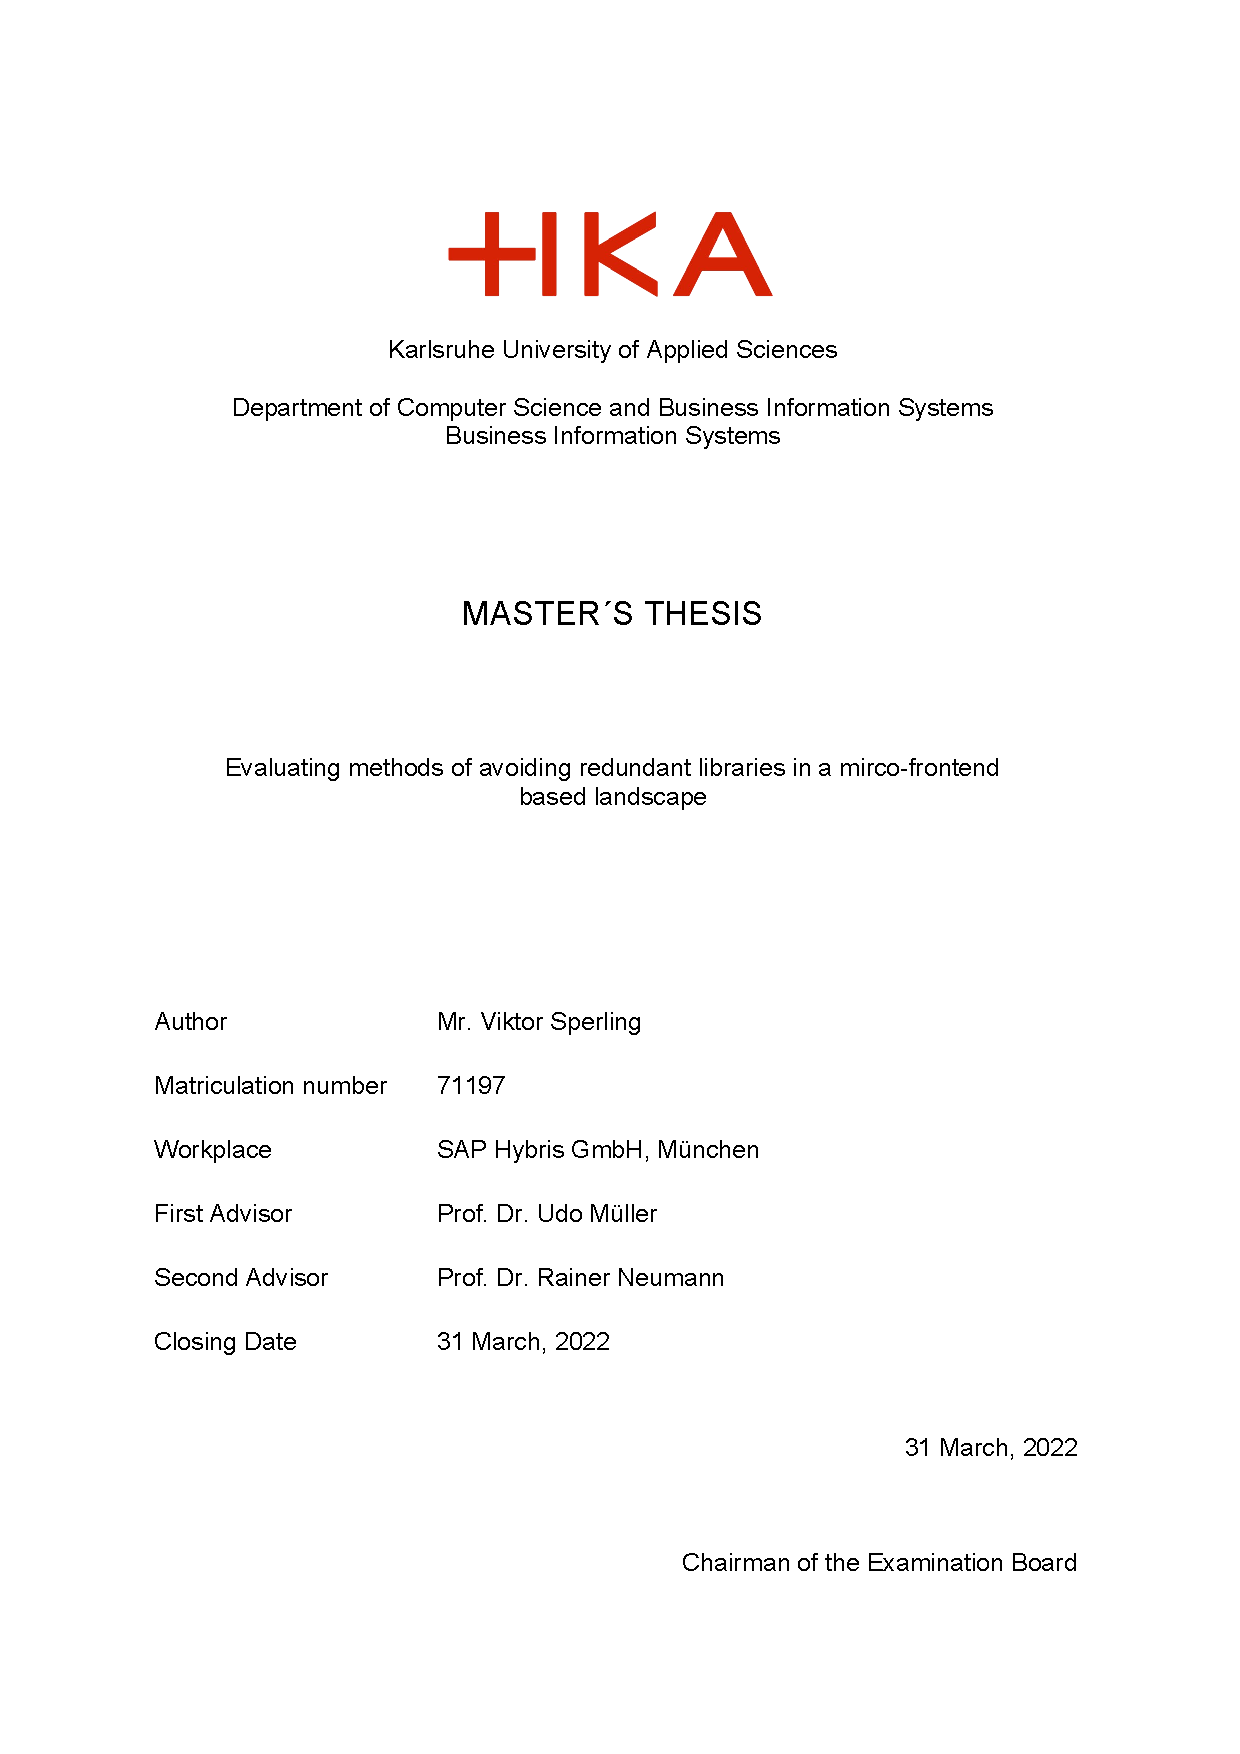
\includepdf[offset=32mm -30mm]{Figures/Thesisdeckblatt.pdf}
	\newpage
	
	\section*{Eidesstattliche Erklärung}
	
	Ich erkläre an Eides statt, dass ich die hier vorgelegte Master-Thesis selbstständig und
	ausschließlich unter Verwendung der angegebenen Literatur und sonstigen Hilfsmittel verfasst habe.
	Die Arbeit wurde in gleicher oder ähnlicher Form keiner anderen Prüfungsbehörde zur Erlangung
	eines akademischen Grades vorgelegt.
	
	\vspace{1.3cm}
	
	\noindent\rule[-0.1cm]{6cm}{0.5pt}\\
	Karlsruhe, den \today
	\newpage
	%----------------------------------------------------------------------------------------
	%	Confidentiality Agreement
	%----------------------------------------------------------------------------------------
%	\section*{Master Thesis Confidentiality Agreement}	
%	Not required yet.
%	Title of thesis:  \textit{Effort analysis of application porting to Kubernetes based on a prototype}
	
%	Name of student: 
%	\textit{Viktor Sperling}
%	Registration no. at university: \textit{48370}, 
%	Course: \textit{Wirtschaftsinformatik}
%	The student is writing a thesis in cooperation with SAP SE (herein: SAP).
%	\textbf{Hochschule Karlsruhe für Technik und Wirtschaft}, represented by its president, and the thesis examiners
	
%	1. \textit{Prof. Dr. Udo Müller} (first examiner),
	
%	2. \textit{Prof. Dr. Rainer Neumann} (second examiner),
	
%	herein: Examiners
%	acknowledge that the thesis and the confidential information about SAP that it contains are trade secrets.

%	The University and the Examiners undertake to treat all unpublished company information, including without limitation technical and business information, plans, experience, knowhow, designs and other documents to which they have access in connection with the thesis as confidential and will not make it available to third parties.        
	
%	The abovementioned duty of confidentiality does not extend to information:
%	1.	That they already knew before this agreement entered force
%	2.	That they rightfully receive from third parties and that is not subject to a duty of confidentiality
%	3.	That is or becomes public knowledge without breach of confidentiality under this agreement
%	4.	That they develop independently
	
%	If university or examination regulations require other examiners to assess the thesis (for example, members of the standing examination committee or university directors), SAP must be informed of their names and they must join this agreement. 
%	The University and the Examiners must mark this thesis as confidential and must not let anyone gain access to it. They must not publish or reproduce the thesis in whole or in part without SAP's express permission. 
%	SAP can bring claims against the University and the Examiners on grounds of a breach of this agreement only if SAP can show their intent or gross negligence.
%	Only German law applies. 

%	First examiner:\hspace{5.4cm}Second examiner:
	
%	\noindent\rule[-0.1cm]{3cm}{0.5pt}\hspace{5cm}\noindent\rule[-0.1cm]{3cm}{0.5pt}\\                      		
%	(Name: Prof. Dr. Udo Müller)\hspace{2.9cm}(Name: Prof. Dr. Rainer Neumann)
		
%	Place: Karlsruhe, den\hspace{4.3cm}				Place: Karlsruhe, den
	
%   Date: \noindent\rule[-0.1cm]{3cm}{0.5pt}\hspace{4cm}Date: \noindent\rule[-0.1cm]{3cm}{0.5pt}
	
	
%	Title of thesis: \textit{Effort analysis of application porting to Kubernetes based on a prototype}
	
%	Name of student: \textit{Viktor Sperling}
	
%	The student is writing a thesis in cooperation with SAP SE. This present thesis on 
	
%	\textit{Effort analysis application porting to Kubernetes based on a prototype}
	
%	contains trade secrets of SAP SE.
%	This thesis has been identified as confidential. Unauthorized persons and organizations are not granted access to this thesis. With the exception of the thesis supervisor, second examiner, and the examining committee of Hochschule Karlsruhe für Technik und Wirtschaft university, no third party is granted access to the thesis or any part of it. The thesis must not be published or reproduced in whole or in part.
	
%	The thesis must not be published, reproduced, or transmitted in whole or in part without the express permission of SAP SE. Only the examiners and the members of the examining committee of Hochschule Karlsruhe für Technik und Wirtschaft university are granted access to this thesis.
%	The confidentiality of the thesis ends no earlier than three months after the publication  and no later than five years after the examination processes are completed.
	
%	\noindent\rule[-0.1cm]{6cm}{0.5pt}\\
%	(Student’s Name: Viktor Sperling)

%	Place: \noindent\rule[-0.1cm]{4cm}{0.5pt} \hspace{3cm} Date:\noindent\rule[-0.1cm]{4cm}{0.5pt}\\
%	\newpage

	
	%----------------------------------------------------------------------------------------
	%	QUOTATION PAGE
	%----------------------------------------------------------------------------------------
	
	%\pagestyle{empty} % No headers or footers for the following pages
	
	%\null\vfill % Add some space to move the quote down the page a bit
	
	%\textit{``Some deep quote \textbf{TO DO}"}
	
	%\begin{flushright}
	%	Add a quote here
	%\end{flushright}
	
	%\vfill\vfill\vfill\vfill\vfill\vfill\null % Add some space at the bottom to position the quote just right
	
	%\clearpage % Start a new page
	
	%----------------------------------------------------------------------------------------
	%	ABSTRACT PAGE
	%----------------------------------------------------------------------------------------
	
	\addtotoc{Abstract} % Add the "Abstract" page entry to the Contents
	
	% \selectlanguage{ngerman}
	% \abstract{ % Add a gap in the Contents, for aesthetics
	
	% Abstrakt Deutsch.
	
	% Mit Absätzen arbeiten.
	
	% }
	
	% \clearpage % Start a new page
	
	\selectlanguage{english}
	\abstract{ % Add a gap in the Contents, for aesthetics
		
		This transcript provides proof of possible solutions regarding redundant libraries in micro frontend landscapes. The data collected is based on an implemented prototype using the Luigi micro frontend framework. Different landscapes, with different technologies are implemented to represent a heterogenic landscape, which is considered to be representative for a micro frontend landscape.
		
		The technologies in use are a Content Delivery Network, the Compound feature of Luigi in combination with Web Components and lastly the Webpack Module Federation, a rather new feature of Webpack which can serve as a foundation for micro frontend architectures.
		After implementation, data is collected and displayed, defining the performance metrics used for the evaluation. It is proven that each of the respective technologies has their own means to avoid redundant libraries in the micro frontend landscapes, be it either distinguishable resource URLs provided by the CDN, reusable Web Components or even shared dependency through the Module Federation. Each technology has its own approach of solving the issue at hand. Still, every method has limitation which are evaluated as well, such as the effort involved when using one of the corresponding technologies.
		
		For CDN, it is shown that even though it is easy to implement and use in the project itself, a public CDN has certain restrictions. These include the absence of special libraries required for the project and the constant dependency on the availability of the CDN servers. Hosting your own CDN involves further costs and requires time for implementation and configuration, which in certain cases might not be affordable.
		Web Components implemented as Compounds in Luigi show great potential in avoiding redundancies to a certain degree, by providing reusable components registered in the browser. Additionally, this technology is framework-independent and compatible with almost all modern browsers, due to its standard status. It is shown how this technology provides a way to support multi-version landscapes via the scoping feature of the UI5 Web Components library.
		The Webpack Module Federation is considered to be a powerful tool to solve the issue of the redundancies in micro frontend landscapes. Not only can it serve to share central dependencies between its federalized modules, but also optimize shared dependencies in different versions. It is assumed that more features can be enabled through the Webpack bundler to optimize the landscape even further.
		
		After showing how each respective technology avoids redundant libraries in a micro frontend landscape, the comparison is made and a conclusion is drawn. The use case and the requirements on the landscape define which technology should or could be used, since all technologies provide a solution for the issue in their own way.
	}
	
	\clearpage % Start a new page
	
	%----------------------------------------------------------------------------------------
	%	LIST OF CONTENTS/FIGURES/TABLES PAGES
	%----------------------------------------------------------------------------------------
	
	\pagestyle{fancy} % The page style headers have been "empty" all this time, now use the "fancy" headers as defined before to bring them back
	
	\lhead{\emph{Content}} % Set the left side page header to "Contents"
	\setcounter{tocdepth}{3}
	\tableofcontents % Write out the Table of Contents
	
	%----------------------------------------------------------------------------------------
	%	THESIS CONTENT - CHAPTERS
	%----------------------------------------------------------------------------------------
	
	\mainmatter % Begin numeric (1,2,3...) page numbering
	
	\pagestyle{fancy} % Return the page headers back to the "fancy" style
	
	% Include the chapters of the thesis as separate files from the Chapters folder
	% Uncomment the lines as you write the chapters
	
	%include chapters here like this:
	% \glsresetall
\chapter{Introduction} % Main chapter title
\label{Chapter1}

\lhead{Chapter 1. \emph{Introduction}}

This chapter will explain the problem, motivation and goals of this transcript. 
It will also narrow down the thesis scope.

\section{Motivation}

The micro frontend technology has experienced a rise in popularity over the past 3 years. The occurrence of such a trend is no surprise, considering the fact that more and more applications are designed following the micro service architecture principles \cite{top_6_frontend_trends}.
Micro frontends share a common interest with their assumed precursor. Generally, it can be stated that the market prefers smaller, independent, lightweight applications over monolithic giants with strong dependencies. Similar to micro services, micro frontends offer almost the same advantages to a development team: Independence of the respective micro frontend teams, shorter and decoupled developments cycles, smaller scope of maintenance, separations of concerns, reusable components available via defined APIs etc.\cite{advantages_of_mfes} However, this concept has certain flaws which have to be considered when making the decision \cite{Yang_2019}.

Depending on the type of the to-be-developed application, the concept of micro frontends is not always favored. One major point of criticism is the aspect of redundancies inside the landscape. Especially, since isolation is a core aspect of this architecture. The circumstance that each micro frontend is a separate project with its own runtime, developed by an independent team, causes this issue to occur. It allows the development teams to use their own preferred tech stack and enables the application itself to be reused in different landscapes. Nonetheless, that also means that isolated micro frontends are partially loading and using the same libraries during their runtime. This is causing an overhead on client and server side and therefore, correlates with the runtime costs of such a landscape and potentially an inferior user experience.\cite{motivation_benefits_adopting_MFs}\cite{micro_frontends_in_general}

Despite isolation being a key aspect of this architecture, it is still possible to avoid the related redundancies without disabling it.

\section{Definition of redundancies}

For the context of this transcript, the term \textit{"redundancies"} or \textit{"redundant libraries"} refers to same libraries or dependencies used by multiple micro frontend projects. For the context of Web Components, it also partially means redundant or reusable code elements, in form of templates or slots.

A library is determined by its identifier or its name, e.g. \texttt{@luigi-project.} If the given library or dependency is imported, by multiple different micro frontends, it is considered to be redundant in the context of this thesis. The case of different versions of redundant libraries is considered too and is covered in subsequent chapters.

\section{Goal}

The goal of this thesis is to provide proof and evaluate methods to avoid redundancies during the runtime of a representative micro frontend landscape. 

To achieve this, two prototypes are implemented using the Luigi micro frontend framework. The landscape itself is designed to be as representative as possible by using a heterogenic tech stack. Additionally, following methods are present to avoid redundantly loaded libraries:

\begin{itemize}[noitemsep]
	\item Content Delivery Network (CDN)
	\item Web Components (WCs) in Luigi Compound views
	\item Webpack Module Federation (WMF) framework
\end{itemize}

The implemented methods are evaluated under predefined metrics. The steps to collect the data for the metrics are explained too.
Eventually, a conclusion is drawn based on the empirical data, accompanied by the subjective opinion of the author. It is explained how the usage and implementation of the respective technologies differs and which advantages each technology offers.
  
\section{Scope of Work}

To account for the limited time frame for this transcript, the following aspects are either not considered or referenced only on a theoretical level.

\begin{description}
	\item[The development of a self-hosted CDN:] An approximate cost assumption is made for such a project, without actual implementation.
	\item[Usage of the Webpack bundler outside the context of the Module Federation:] Since this bundler offers many ways for configuration, the focus lies on those necessary for the WMF context. 
	\item[Configuration for the Luigi framework of the implemented landscape:] Each implemented prototype uses this framework for its micro frontend landscapes. Since showing all configurations would be to extensive, only a general overview is given. 
	\item[Development of WCs:] The general usage and functionality of this standard is explained. 
	\item[Combinations of the implemented technologies:] This aspect is not empirically considered in this transcript. 
\end{description}

\section{The collaborators}

This thesis was written in collaboration with SAP Luigi project team. The SAP was originally founded in in 1972 as SAPD (system analysis program development), later became SAP AG in 2005 and in 2014 SAP SE. The Hybris company was originally founded in 1997, was later acquired by SAP in 2013, after moving its headquarter from Zug in Switzerland to Munich in Germany.\cite{sap_history} The Luigi project team is part of the SAP Hybris organization but the developed framework is an open-source product. 
The team and their product aim to improve the experiences of customers, developers and administrators who are using Luigi. Their open-source product was designed to make the transformation from monolithic architectures into micro frontend based landscapes as smooth as possible. 

 

	% \glsresetall
\chapter{Micro frontend framework Luigi} % Main chapter title
\label{Chapter2}

\lhead{Chapter 2. \emph{Micro frontend framework Luigi}}

In this chapter, an overview about the used Luigi framework is given.

Currently there are different micro frontend frameworks available on the market, including but not limited to \textbf{Bit, SystemJS, Webpack 5 Module Federation, Piral, Single SPA} and \textbf{Luigi}.\cite{top10_mffs}
For the implementation of the representative landscapes the Luigi framework was used. Therefore, a short introduction to Luigi it is given here.

\section{Luigi}

Luigi is an open-source JavaScript framework for micro frontends, consisting of two main parts, the \textbf{Luigi Core} and the \textbf{Luigi Client}. It provides a basis to integrate micro frontends, also called \textbf{Nodes} in this context. Both parts serve different purposes in the micro frontend landscape.\cite{luigi_doc_overview}

\subsection{Core}

The \textbf{Luigi Core} is the basis of the whole landscape. It defines the main app, which will serve as an entry point for the user. The possibilities for, applicable configurations of this part are the following:

\begin{itemize}[noitemsep]
	\item Navigation - enables navigation between micro frontends
	\item Authorization - enables authorization for the landscape
	\item Localization - providing translations to display its applications in multiple languages
	\item General settings - e.g. header display configurations, enable loading indicators for the micro frontends, etc.
	\item Luigi Core API - providing functions for the core app to interact with the framework and access its features
\end{itemize} 

The core application inside the landscape is determined via the \texttt{luigi.config.js}. Any project containing it can fulfill this role, which is the only prerequisite. In the context of the framework, this app is later referred to as the \textbf{Core}.
Following this principle, the project structure of the \textbf{Core} could look as shown in listing \ref{list:luigi_core_structure}.\footnote{This example is taken directly from the implemented core project.}  

\begin{lstlisting}[language=Bash, caption=Project structure for a Luigi Core application including the \texttt{luigi.config.js}, label=list:luigi_core_structure,  xleftmargin=.0\textwidth, xrightmargin=.0\textwidth]
	- react-core-mf
		- [...]
		- node_modules
		- public
			- [...]
			- index.html
			- luigi.config.js
		- [...]
		- src
\end{lstlisting}

In the \texttt{luigi.config.js} itself the above mentioned possible configurations are defined.\cite{luigi_doc_core}

\subsection{Client}

The Luigi Client serves as the connection between the framework and its micro frontends. In order to establish the connection, a micro frontend has to import and initialize the Client. This will grant the micro frontend access to the \textbf{LuigiClient} object during the runtime. The micro frontend can then interact with the framework to e.g. set a global state, add event listeners or enable navigation between other micro frontends in the landscape.

An import of the Luigi Client can be accomplished via different methods. The most straightforward approach is the direct import with a HTML script tag. Another option would be the import of the local package manager dependency.\cite{luigi_client}

\begin{lstlisting}[caption=Import methods of the Luigi Client, label=list:import_luigi_client,  xleftmargin=.0\textwidth, xrightmargin=.0\textwidth]
	<!-- Via a HTML script tag -->
	<script src="https://unpkg.com/@luigi-project/client@1.17.0/luigi-client.js">
	</script>
	
	<!-- Via a package manager -->
	import LuigiClient from "@luigi-project/client";
\end{lstlisting}

\section{Architecture}

After the short introduction of the framework's core components, a general architecture of a landscape using Luigi is provided in figure \ref{fig:luigi_architecture_fig}.

\begin{figure}[!h]
	\centering
	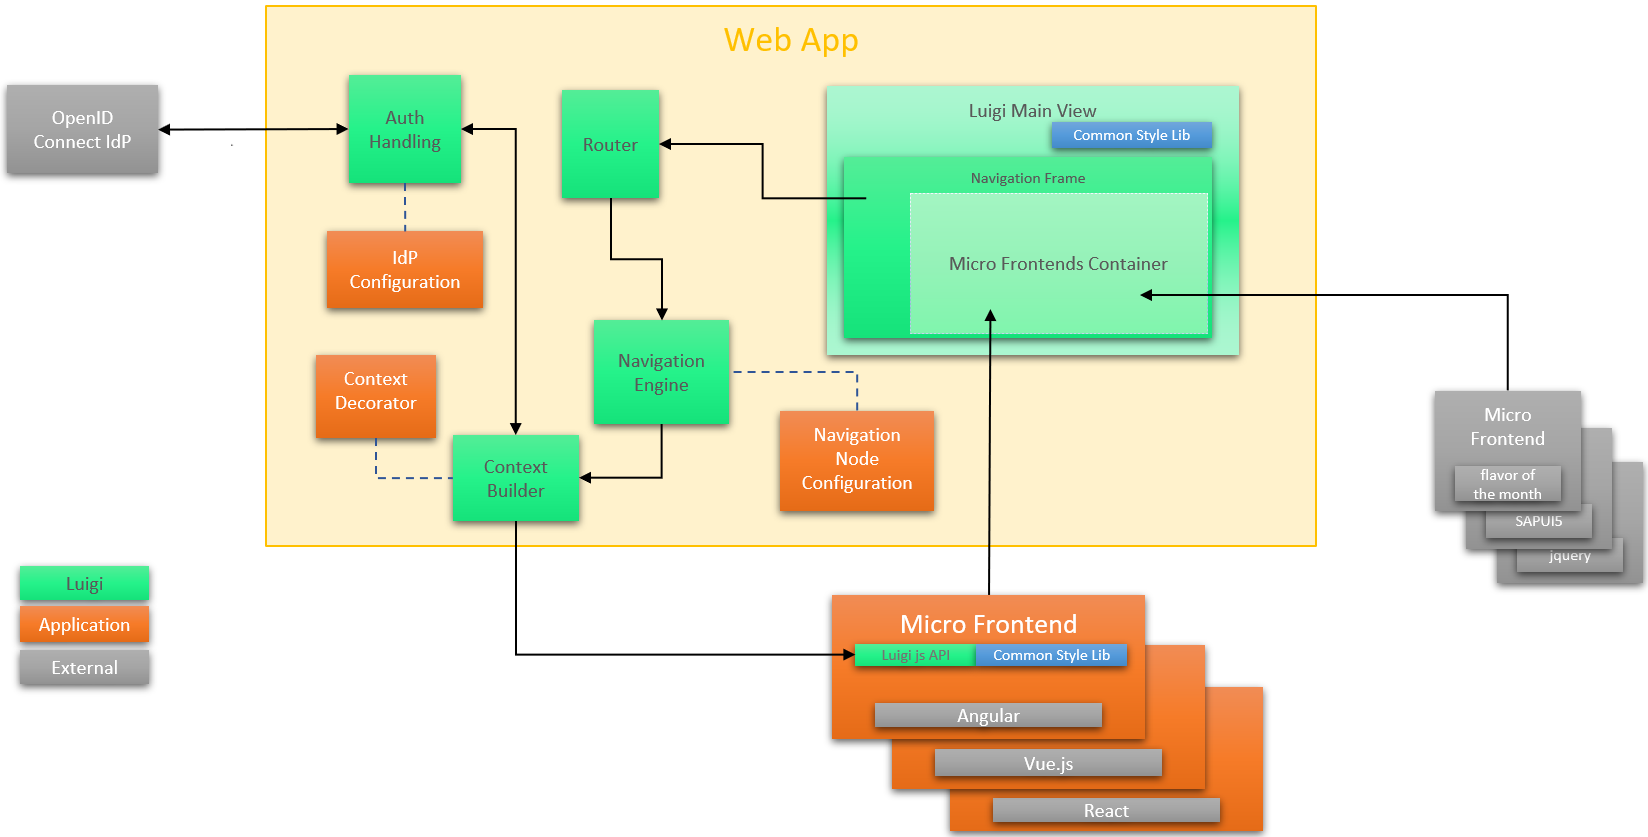
\includegraphics[width=1.05\textwidth]{Figures/Luigi_Architektur.png}
	\caption{Architecture of the Luigi Framework \cite{luigi_architecture}}
	\label{fig:luigi_architecture_fig}
\end{figure}

As can be seen in figure \ref{fig:luigi_architecture_fig}, the displayed micro frontends in the Web App have a distinguished position in the Micro Frontends Container. The embedded projects can either be integrated via iFrames or as Web Components.
Via the provided dashboard (Navigation Frame), the Luigi Core features are used. Through it, the navigation or search feature can be accessed.

As described in the first chapter of this transcript, the issue in such a landscape are the redundantly imported libraries of the embedded micro frontends. The reason for this problem is that each node is an isolated application.
For instance, navigating to the first micro frontend, followed by the second one, will load the bundled projects with their corresponding dependencies. In this case, the browser has no way to distinguish if a loaded resource is already present or not. The reason for that is the bundling of projects which makes the references indistinguishable to the browser.
The following chapters will introduce technologies, which offer methods to resolve this issue. 
 

	% \glsresetall
\chapter{Content Delivery Networks} % Main chapter title
\label{Chapter3}

\lhead{Chapter 3. \emph{Content Delivery Networks}}

One way of avoiding redundant libraries can be a central repository, where all resources are stored and can be requested via an API. Such a concept exists in the idea of Content Delivery Networks (CDNs).
Since the resources are loaded via the CDN API, a dependency is available under a unique URL. Loading a dependency twice means the browser requests the resource from the same URL with the same parameters. Therefore, the browser can determine if the given resource is already present and decide to either load it from the CDN or from the browser cache, if it is already loaded.\cite{caching_in_browser}

Nonetheless, a CDN has its limits which have to be considered. Costs can play a key role in the decision process.
Even though free CDN services like \textbf{Unpkg.com} or \textbf{cdnjs} are valid options, the advantages of using these might differ depending on the business case.
For instance, those services might solve the issue of redundant libraries in a micro frontend landscape, but do not necessarily improve the user experience of the application. 
Since the resources would be loaded from a cloud based service, the server location has significant influence on the latency of the requests. Therefore, depending from where the website is accessed, this circumstance could lead to a performance decrease when initially loading the page.\cite{cdn_general}

Also the technological dependency on a public cloud based CDN has to be considered. Most cloud based services are scalable and replicable. However, a down time could lead to immense costs for a platform provider relying on a public CDN to deliver the platform resources.
Besides, it is never guaranteed that certain dependencies are always available on the public CDN.

Another option is self-hosting a CDN and providing all required resources independently. A business would need to acquire hardware-resources (physically or via a hardware-as-a-service provider like Amazon Web Services), maintain the servers, fill the CDN with the necessary content and keep it up to date. However costs attached to this scenario can be immense and exclude this method due to cost inefficiency.\cite{Meassuring_a_commercial_CDN}

This chapter will give further information about the CDN technology, how it functions and what further features it offers to optimize a micro frontends or websites performance.

\section{Architecture}

The basic architecture of a CDN can be split into three different building blocks.

\begin{description}
	\item[Point of Presence (PoPs):] Strategically located data centers around the world. Their function is to reduce the round trip time of requests. PoPs usually consist of several caching servers.
	\item[Caching servers:] These servers are located in different PoPs and serve the function of caching resources from the origin server. That way website loading times and bandwidth allocations are reduced.
	\item[Hardware, like SSD/HDD and RAM:] Located in the cache servers, the purpose of this building block is to provide the necessary storage and computing capacity. Better hardware means faster computing time, which then again improves the overall performance of the designated caching server.
\end{description}

Besides the above three building blocks, another one is crucial for the architecture of a CDN: The \textbf{origin server}. In a CDNs topology, the origin server can be compared to the center, or core. This is the server onto which the CDNs content is uploaded, synced with or distributed over the CDNs caching servers.\cite{cdn_origin_server}

An example for a basic CDN distribution is shown in figure \ref{fig:cdn_general_arch}.

\begin{figure}[!h]
	\centering
	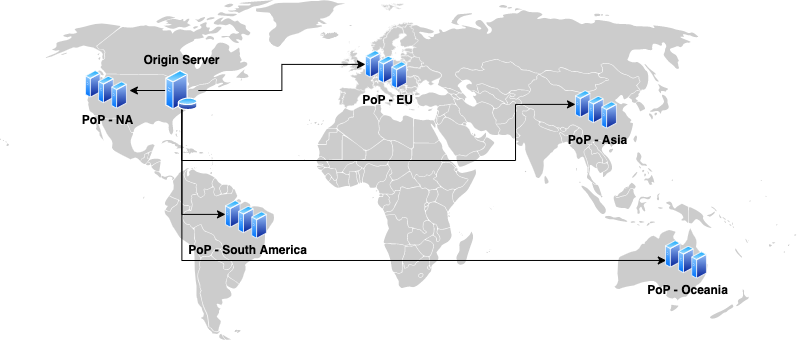
\includegraphics[width=1\textwidth]{Figures/basic_cdn_arch.drawio.png}
	\caption{Basic distribution of a CDN}
	\label{fig:cdn_general_arch}
\end{figure}

It has to be mentioned that the geographical distribution in figure \ref{fig:cdn_general_arch} is simplified, for the sake of readability. In a real scenario, the cache servers of each PoP would themselves be distributed over different data centers on the continent. A client requesting resources from the CDN always communicates with the nearest possible cache server to their designated location.\cite{cdn_general}

\section{Design}

For a CDN to fulfill its purpose, four requirements have to be met. These are not only technical requirements, like necessary hardware, but rather concerning the general design of the CDN.
The four pillars of CDN design are:

\begin{description}
	\item[Performance:] First and foremost, the CDN has to provide a benefit when it comes to website performance. When the usage of a CDN increases the loading time of a website, the negative effect on user experience can cause financial harm to the host.\cite{cdn_general}
	\item[Scalability:] Since a cache server can serve multiple resources to different websites, it has to be able to handle traffic peaks. Without the aspect of scalability (either horizontal or vertical), this requirement cannot be met which would affect the CDNs performance.
	\item[Reliability:] A website host has to rely on the CDN to deliver the websites resources. An outage on CDN side would cause the same effect to the relying websites, resulting in additional losses for the designated hosts. Therefore, most CDN providers commit to 99.9\% availability in their service level agreements (SLAs).
	\item[Responsiveness:] The aspect of responsiveness targets the issue of synchronization inside the CDN. A CDN has to be capable to react to changes and distribute those to its PoPs over the globe accordingly. Otherwise inconsistencies could occur on the websites relying on the CDN. This is ensured through an automated pull mechanism, via which edge servers pull changes from the origin server.\cite{cdn_origin_server}
\end{description}

Additionally to those four requirements, the topology of a CDN has to be considered. There are two options which can be used. Both would serve their purpose, but have different advantages as well as disadvantages. 

\begin{description}
	\item[The scattered CDN:] This topology focuses on physical proximity. The PoPs are kept rather small in size, but are scattered around the world in greater frequency, thus providing as much proximity to their clients as possible. This topology excels in providing the CDN's resources into low-connectivity regions, since it is not highly dependent on wire infrastructure. When it comes to latency, it does not suffer as much due to the short distance between client and server. The trade-off with this topology is that it accrues more maintenance costs, since more PoPs are required to be maintained. Also, deploying new configurations can be connected to a lot of effort, depending on the number of PoPs scattered across the CDN. 
	Additionally, this number can also affect the RTT since every PoP inbetween the client and the server is a connection point.
	
	\item[The consolidated CDN:] Contrary to the scattered CDN, this topology is designed to consolidate its resources at strategically located data centers. Since the PoPs are only located in those major data centers, the servers available to the PoPs are highly advanced and provide a lot of hardware capacity. Additionally, since the number of major data centers around the world is rather limited, the number of PoPs is reduced as well, compared to the scattered topology. Following the quality over quantity principle, a PoP in this topology can handle a greater amount of traffic compared to its counterpart, and is also more resilient, specifically when it comes to DDoS attacks. Also, due to the moderate number of PoPs, it is easier and faster for the operators of the CDN to deploy new configurations.
	Nonetheless, the trade-off for this topology is that, even though it can handle a high number of requests, its reach to low-connectivity regions is rather limited. This is due to the proximity difference between the servers and clients. Additionally, deploying a new PoP into this topology requires more effort, since the PoPs are rather complex.	
\end{description}


The design decision is of course dependent on the business case for the CDN, as both topologies are intended to solve specific issues or challenges. \cite{cdn_architecture} 

\section{Optimization}

The CDN technology offers several ways of optimizing a websites performance and therefore, improving the user experience. In the following sections these optimizations will be showcased and explained.

\subsection{Route optimization with Anycast}

As previously mentioned, a CDN can be designed with different topologies which can affect its performance. Another factor which has to be considered in this equation is the routing itself. Basically, it does not matter if a cache server is located in close proximity to a client, if the requested resource is not present there. In this case, the client would have to be routed to different, cache servers located further away. 
To circumvent this, the Anycast routing is used in modern CDNs. This traffic routing algorithm is best explained in direct comparison with Unicast. Both serve the same purpose of routing requests to their designated destination, but they do it in different ways. Where with Unicast each node has a unique address, Anycast advertises multiple nodes with the same address.
For instance, in a Unicast orchestrated network the server address \texttt{10.10.0.1} would be only present once. Anycast, on the other hand, would advertise this exact address over multiple different servers around the globe. Thus, a request towards the address would reach its destination via the shortest path, given that the path will be identified and prioritized by devices that actually govern the flow of traffic.
The shortest path itself is counted in hops. Hops represent the number of time a request changes hands between hosts.\cite{cdn_route_opt}

\subsection{TLS Performance}

The route optimization with Anycast, also improves the RTT when using the TLS/SSL protocol. Since this section does not focus on explaining the protocol, only a short description is given.
SSL (Secure Socket Layer) or, as it now should be called, TLS (Transport Layer Security) is a protocol via which secure communications are ensured on the Internet. The communicating parties establish a connection via the following steps:

\begin{enumerate}[noitemsep]
	\item A so-called three-way handshake is done
	\item The parties agree upon an encryption method
	\item Mutual verification process is performed
	\item Symmetric keys for encoding and decoding are generated
\end{enumerate}

These steps are necessary to ensure secure communication and are a welcome trade-off for the benefits they provide. 

A CDN can provide improvement to this overhead and decrease the RTT of a request. Through the aspect of route optimization and general proximity, the overall request distance is decreased. Therefore, the RTT is shortened as well. The steps are still processed, they just do not have to travel that long. Additionally, the SSL/TLS negotiation process is shorter, too.\cite{cdn_ssl_tsl}

\subsection{Frontend optimization}

The term frontend optimization refers to the process of making a website more browser-friendly and reducing loading times. There are multiple ways to optimize a frontend. These will be explained under consideration of the role a CDN plays in them.


\begin{description}
	\item[Reducing HTTP requests:] When loading a website, the browser opens several HTTP connections, the number of which is actually limited by the browser. If a website requires more connections than a browser can open at the time, the browser has to start queuing the rest. This again leads to longer loading times and affects the user experience. A CDN improves on that by pre-pooling connections and ensuring they remain open throughout a session. Even though this does not reduce the actual number of requests, it does improve the response time for each one, making it so that every request can be processed faster. Additionally, HTTP/2 introduces the method of multiplexing. This allows a single TCP connection to transfer multiple different HTTP requests \cite{http2}.
	
	\item[File compression:] Not only do the number of requests or the proximity of the client to the server, affect the responsiveness of a website. The actual content has a major role in this aspect, too. Loading one single resource with a size of 1 GB takes a while, even if the server is close by. Reducing the size of this file or resource might increase the loading process. File compression like gzip is a method of doing exactly that. Most modern CDN providers offer automated file compression with gzip to reduce the actual content size delivered to the client.
	
	\item[Cache optimization:] Via caching, static files are stored either on the client device or in the cache of a nearby cache server. Locally stored static files do not have to be loaded via the network and are available to the browser for rendering almost immediately. The only question remaining is how long does a resource have to be cached. This information is necessary to optimize the use of the client's cache. The caching time is usually defined in the cache header of the request. Modern CDNs offer cache control options, which help in defining rules for exactly that header.
	CDNs have also started to use machine learning techniques to follow and understand content usage patterns and automatically optimize caching policies.
	
	\item[Code minification:] Similar to the file compression method, the process of code minification offers a way of reducing file sizes too. Whereas a developer writes code in a humanly readable way, with spaces and line breaks, a machine does not need this kind of formatting. By removing comments, spaces and line breaks, the size of a code file can be reduced by 30\%. CDNs use methods like gzip, minify or a combination of these two to reduce the size of JavaScript, HTML or CSS files.
	
	\item[Image optimization:] Images can be immense in size and require a long time to load. The best way to display an image on a website would be to cache it first and then load it from the cache to reduce actual loading time through the network. Another option could be to reduce the actual size of the image and thus the loading time.
	However, other than code files, images are already compressed when loaded, therefore compressing them further to reduce file size might cause a loss of image quality. This is called lossy compression. If this trade-off is not an option, caching would be more effective.
	CDNs offer exactly that solution, caching images and providing them from the nearest source available to the client. If this does not suffice, CDNs also offer a progressive rendering option for images. On initially loading the page, the CDN would provide a lossy compressed version of the image quickly and then progressively replace it with higher-resolution variants.
	Alternatively, a website host could use vector or raster images. These are resolution independent, smaller in size and highly responsive.\cite{cdn_fe_opt_img_opt}
\end{description}

These methods in combination with the CDN technology provide a possible gain in user experience for a website host. \cite{cdn_fe_opt}

\section{Hosting a CDN}

Even though the method of a self-hosted CDN was not implemented in the developed prototype, it has to be considered for the context of this thesis. Since the basic principle of a CDN was already explained, this section will focus on the financial aspect of the technology.

This topic will be showcased based on a hypothetical scenario. The numbers and metrics of this scenario are either assumed or taken directly from the implemented prototype.

The first requirements of the scenario are the following:

\begin{itemize}[noitemsep]
	\item A micro frontend landscape has to be developed. 
	\item To reduce the runtime costs, the loading of redundant libraries should be avoided in the landscape.
	\item The libraries for the landscape were developed by the same team and are only available for internal use.
\end{itemize} 

These circumstances ensure that only a self-hosted CDN is applicable.
Next, the numbers and further requirements of the landscape are necessary. Those are required for the cost calculation of the CDN.
It is mentioned if the numbers are actually \textit{assumed/estimated} or \textit{taken from the prototype}.

\begin{itemize}[noitemsep]
	\item How often the site is accessed per day - $50 000$ times (estimated)
	\item Avg. byte size per page load without caching on client side - $8983.5$ KB (taken from the prototype)
	\item Avg. amount of GET requests to CDN per site load - $198$ requests (taken from the prototype)
	\item The site is only accessed in North America 
\end{itemize} 

Based on those requirements, the following values are calculated for the monthly CDN usage of the described scenario landscape.

\begin{quote}
	\begin{center}
		Let $A$ be the amount of requests to the CDN per month:
		\begin{math}
			A = 50000 \times 30 \times 198 = 297000000
		\end{math}
	\end{center} 
\end{quote}

\begin{quote}
	\begin{center}
		Let $B$ be the amount of bytes loaded per month:
		\begin{math}
			B = 50000 \times 30 \times 8983.5 = 13475250000 \: $KB$ \; = 13.47525 \: $TB$
		\end{math}
	\end{center} 
\end{quote}

Next, it will be calculated how much it would cost a company or department to pay for the CDN defined in this scenario.

There are multiple CDN solution providers on the market, including \textbf{Amazon CloudFront, Azure CDN, Google Cloud CDN}. \cite{top_10_cdn}
Since the pricing models of the mentioned providers differ, it is difficult to compare them directly. Applying the given scenario to the pricing calculator of the respective providers results in the following numbers.

\begin{itemize}[noitemsep]
	\item Amazon CloudFront - $1426.22$ \$ per month
	\item Google Cloud CDN - $1168.99$ \$ per month
	\item Azure CDN - $1123.90$ \$ per month
\end{itemize} 

After averaging those values an $Avg. price$ is calculated.  

\begin{quote}
	\begin{center}
		\begin{equation*}
			Avg. price = 
			\frac{
				\left(1426.22 + 1168.99 + 1123,90\right)
			}{
				3
			} = 1239.70 \: \$
		\end{equation*}
	\end{center} 
\end{quote}

It has to be mentioned that these values were calculated using the basic packages offered by the providers. There are further features which can be added to the solutions, which of course would increase the sum. Additionally, other providers have different pricing models, some of which include pricing depending on the HTTP requests sent to the CDN. Others charge prices when resources are stored in several PoPs around the world. Also, locations play a key role, as different regions pay more for traffic then others and this value is provider-specific.
Since it is not the goal to pick a provider here, but rather to provide a general overview of costs for such a solution, those additional features were not considered for the given scenario.




	% \glsresetall
\chapter{Web Components} % Main chapter title
\label{Chapter4}

\lhead{Chapter 4. \emph{Web Components}}

As in \ref{Chapter2} introduced, Web Components have the attribute of the Custom Element, via which the individuality of each registered tag is guaranteed.
Nonetheless to understand the actual functionality of Web Components, it is necessary to explain the other aspects of it.
The following section will introduce the other three standards of Web Components and their functions and showcase how exactly they serve a purpose for the context of the thesis.

\section{Shadow DOM}

The DOM (Document Object Model) represents the elements of a markup document in a tree-like structure, consisting of connected nodes. The commonly used markup language for websites is HTML. \cite{wc_shadow_dom}
The Shadow DOM is also a DOM, but is attached to the actual DOM of the document. Underneath it, elements can be defined the same way as they are in the regular DOM. The difference appears during the rendering of the document, when a page is loaded. The Shadow DOM elements are rendered separately from the DOM it is attached to.\cite{simon_thesis}

To understand the relationship between the two connected DOMs following terms have to be explained.

\begin{itemize}
	\item \textbf{Shadow host} - The attachment of the Shadow DOM to the normal DOM happens via a node inside the normal DOM.
	\item \textbf{Shadow tree} - Since the Shadow DOM is a DOM in itself, it consists of nodes in a tree-like structure.
	\item \textbf{Shadow boundary} - The Shadow DOM capsules its Shadow tree an renders it separately from the actual DOM. This encapsulated area defines where the Shadow DOM begins and ends.
	\item \textbf{Shadow root} - Just like a regular DOM a Shadow DOM has a root from where it originates.
\end{itemize} 

Figure \ref{fig:shadow_dom} visualizes the relations between the newly introduced terms.

\begin{figure}[!h]
	\centering
	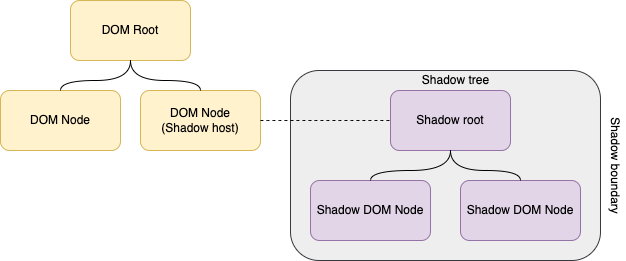
\includegraphics[width=1\textwidth]{Figures/shadow_dom.drawio.png}
	\caption{Shadow DOM architecture}
	\label{fig:shadow_dom}
\end{figure}

Through the isolation of the Shadow DOMs code, this standard offers a way to provide scoped HTML and CSS code to custom elements. As mentioned before, the nodes of the Shadow DOM are rendered separately. Therefore, styles, ids, names or even CSS classes and other configurations applied to a tag inside the Shadow DOM are not applied to the actual DOM.

Listing \ref{shadow_dom_definition} provides be a simple example.

\begin{lstlisting}[caption=Definition of a custom element using the Shadow DOM \cite{simon_thesis}, label=shadow_dom_definition]
<!DOCTYPE html> 
	...
	<body>
		<p>Plain</p> 
		<custom-element></custom-element>
		
		<script>
			class CustomElement extends HTMLElement {
				constructor() { 
					super();
					const shadow = this.attachShadow({mode: 'open'}); 
					shadow.innerHTML = `<style> p {color: red;} </style>`; 
					const shadowParagraph = document.createElement('p'); 
					shadowParagraph.textContent = 'Blue'; 
					shadow.appendChild(shadowParagraph);
				}
			}
			customElements.define('custom-element', CustomElement); 
			customElement = new CustomElement(); 
			console.log(customElement.shadowRoot)
		</script>
	</body>
</html>
\end{lstlisting}

The listing shows the usage of the Shadow DOM in combination with registering a custom element (named \texttt{custom-element}) using the customElements API which was explained in chapter \ref{Chapter2}.
The \texttt{script} tag of the snippet starts with creating a new HTML element called CustomElement. It is an extension to the HTMLElement class. This new element has the Shadow DOM attached to it. Therefore, it is the Shadow host in the DOM tree. Via the \texttt{innerHTML} attribute a Shadow DOM Node is created. In this case it is a styling for paragraphs,followed by the creation of a paragraph onto which the styling is applied. Additionally the text color of the paragraph is set to blue and lastly it is attached to the Shadow root.
The last three lines of the script, are the definition and registration of the new \texttt{custom-element}, the creation of a new \texttt{customElement} object and the output of the attached Shadow DOM in the console.

Now when looking at the body of the above snippet, it becomes visible that beside the \texttt{custom-element} another paragraph is defined in the document. Usually the styles defined in the \texttt{script} below would apply to this paragraph, too. Through the encapsulation of the two separate DOMs this is not the case. The paragraph defined in the body of the document will be completely unaffected by the changes applied to the paragraphs in the Shadow DOM.\cite{simon_thesis}

Now another configuration which is shown in the snippet is the \texttt{this.attachShadow({mode: 'open'})}. This mode property defines the visibility of the Shadow DOM to the browser. If set to \texttt{open}, the elements of the Shadow DOM can be inspected inside the sources. Thus, the \texttt{console.log(customElement.shadowRoot)} line would work if executed. 
If the mode would be set to \texttt{closed}  the \texttt{console.log()} command in line 20 would return \texttt{null}.\cite{simon_thesis}

This behavior is not meant to be used as a measure of security, since it can be overwritten. The Shadow DOM encapsulates every part of its DOM elements, that means HTML, CSS and JavaScript. The \texttt{document} object, available during runtime, stays the same for the regular DOM as for the Shadow DOM though. Therefore, each configuration done in the Shadow DOM via scripts can be easily overwritten from any other script in the document, thus the mode can be changed even if initially set to \texttt{closed}.\cite{shadow_dom_encapsulation} For Web Components in particular it is not recommended to use this mode at all, since it would make them less flexible for end users.\cite{wc_shadow_dom_google}

This feature can be used in combination with a component library like UI5 Web Components, to customize styles or appearances of individual components. Nonetheless, for the context of this thesis, it does not serve any purpose to actually avoid redundancies in a micro frontend landscape, instead it might even increase them. The encapsulation of code elements between the single components increases the isolation and thus it cannot be guaranteed that e.g. the same CSS class is not rendered in multiple different Shadow DOMs. Even though the redundancies would occur on code level and not on dependency level, they are redundancies nonetheless.

\section{HTML Template}

This standard offers a way to define reusable markup code. As a part of the HTML standard itself, the \texttt{template} tag is used to define templates. These are not rendered unless used by another element. Similar to \texttt{template}, \texttt{slot} serves the same purpose, but in a different way. Templates are defined HTML code snippets which can be cloned and inserted in other document elements or even elements rendered in the Shadow DOM.
Slots on the other hand serve as placeholder for either default markup texts or other DOM elements. Therefore, a template is a rather static piece of reusable HTML code, compared to slots.
Slot themselves are identified by their name, the content is inserted when the slot is addressed by its name.
Listings \ref{template_example} and \ref{slot_example} provide examples how exactly these two standards are used. \cite{wc_html_template_slots}

\begin{lstlisting}[caption=Definition and usage of the \texttt{template} standard \cite{wc_html_template_slots}, label=template_example]
<!-- Definition of the template -->
<template id="my-paragraph">
	<p>My paragraph</p>
</template>

<!-- Usage of the template in an Web Component -->
customElements.define('my-paragraph',
class extends HTMLElement {
	constructor() {
		super();
		let template = document.getElementById('my-paragraph');
		let templateContent = template.content;
		
		const shadowRoot = this.attachShadow({mode: 'open'})
		.appendChild(templateContent.cloneNode(true));
	}
});
\end{lstlisting}

It is important to note, that the defined template in the listing is not rendered unless somehow included in a DOM (either Shadow DOM or the regular DOM), via Java Script.

\begin{lstlisting}[language=HTML5, caption=Definition and usage of the \texttt{slot} standard \cite{wc_html_template_slots}, label=slot_example]
<!-- Definition of the slot -->
<p>
	<slot name="my-text">Default input</slot>
</p>

<!-- Usage of the slot in the markup document -->
<my-paragraph>
	<ul slot="my-text">
		<li>Some different input</li>
		<li>In a list!</li>
	</ul>
</my-paragraph>
\end{lstlisting}

As it can be seen in \ref{slot_example}, the \texttt{slot} definition has some default content defined. In the above case it´s a simple text. When the slot is used, this content is overwritten by the content in the element which is calling the \texttt{slot} by its name.
In that case the content is replaced by some list items.
Other than the templates, slots are always rendered if included in the markup via their respective names. The content which is rendered is depended on, if the default content is overwritten or not.

Even though slots are a HTML standard just as templates, their support for browsers is not always guaranteed. This is due to the fact, that compared to templates it is a rather new standard.

In combination these two standards offer a way to define flexible, reusable markup code for Web Components.\cite{wc_html_template_slots} 

When developing own Web Components for a micro frontend landscape, this aspect can be used to reduce repetitive HTML code elements by serving them a templates. But again this feature is not applicable when it comes to reducing redundant libraries in a micro frontend landscape. Redundant code snippets can be defined as reusable templates but not the actual libraries.

\section{ES Modules}

The last standard is not referred to by every source, but according to \cite{wc_specifications}, it is a stable part of the Web Components standard, via which Java Script modules can be defined and reused by other documents.
Thus the development of Web Components can be done in a modular way, making every component available to other documents, using the \texttt{type="module"} attribute.

\begin{lstlisting}[language=HTML5, caption=Importing modular Java Script documents into another \cite{wc_specifications}, label=es_modules_example]
<!-- Import of the JS Module -->
<script type="module" src="awesome-explosion.js"></script>
	...
<script type="module">
	import 'awesome-explosion.js';
	...
	import {awesomeExplosion} from '@awesome-things/awesome-explosion';
</script>

<!-- Usage of the newly imported module -->
<awesome-explosion>
	...
</awesome-explosion>
\end{lstlisting}

Listing \ref{es_modules_example} shows such an import. Assuming the \texttt{awesome-explosion.js} files contains the definition of an element called \texttt{awesome-explosion}, these lines enable the document to use this element.\cite{wc_specifications}

This feature is essential for the prototype developed, since via this aspect the components are made available to the landscape. The used Web Components are served as ES Modules to the landscape and are imported similarly as shown in \ref{es_modules_example}. Therefore, this aspect enables a component to be imported in multiple micro frontends as a module.

\section{Usage of Web Components in the Prototype}

The Web Components standard was partially used in the development of the prototype. This technology was used to embed the developed components as part of a compound view, using the corresponding feature in Luigi. \cite{luigi_wc} \cite{luigi_compound}
For development itself no UI application framework was used, which means all three compounds were developed using plain Java Script. The actual components used in the micro frontends of the compounds, were taken from a component library called UI5 Web Components. Each element in that library is in fact a Web Component.\cite{ui5_wc_github}
Consisting of the picked elements and under the usage of the scoping feature of the component library, the compounds where created. This made it possible to scope the tags of the UI5 Web Components.\cite{ui5_webcomponents_scoping}

\begin{lstlisting}[caption=Scoping feature used in the prototype, label=scoping_wc_prototype]
import { LuigiElement, html } 
from "@luigi-project/client/luigi-element.js";
import { setCustomElementsScopingSuffix } 
from "@ui5/webcomponents-base/dist/CustomElementsScope.js";
setCustomElementsScopingSuffix("placeholder");
import "@ui5/webcomponents/dist/Dialog.js";
import "@ui5/webcomponents/dist/Button.js";
[...]

export default class extends LuigiElement {
	constructor() {
		super();
		[...]
	render() {
		return html`
		<div>
			<div class="header">
				<h2>Products table - Version: placeholder</h2>
			</div>
			
			<ui5-table-placeholder id="ui5-table" 
			ui5-table sticky-column-header>
				<!-- Columns -->
				<ui5-table-column-placeholder 
					slot="columns" 
					style="width: 4rem">
					<span 
					style="line-height: 1.4rem">
						Product
					</span>
				</ui5-table-column-placeholder>
				
				[...]
				
			</ui5-table-placeholder>
		</div>`;
	}
}
\end{lstlisting}

Listing \ref{scoping_wc_prototype} shows the exact usage of the scoping feature. 
The imported \textit{setCustomElementsScopingSuffix} function enables to define a custom suffix to all UI5 Web Component elements, if not configured otherwise. Also, as it can be seen in the same listing, the suffix is set to \textit{placeholder} using the imported method 
\textit{setCustomElementsScopingSuffix("placeholder")}.
This is done for the sake of the experiment itself. It was intended to deploy six same or similar looking Web Components into the Luigi landscape to test how many redundancies occur. In addition it was meant to be tested how different versions of the same elements could be registered. For example the \textit{Bar} element in version \textit{1.0.1} is registered under same tag as the same element in version \textit{1.1.0}. This scenario has to be handled and the scoping feature is one way of doing so.
By defining a version suffix for the \textit{Bar} element tag, the browser can distinguish those elements.
In case of the prototype to create this exact scenario, one global tag suffix \textit{placeholder} was picked and later replaced. The replacement itself happened during the bundling of the project. The RollUp bundler provided the necessary functionality for that.
Inside the \texttt{rollup.config.js} several configurations were defined, which are shown in listing \ref{rollupconfigjs}.

\begin{lstlisting}[language=JavaScript, caption=Content of the \texttt{rollup.config.js}, label=rollupconfigjs]
imp\part{ort resolve from '@rollup/plugin-node-resolve';
import json from '@rollup/plugin-json';
import url from "@rollup/plugin-url";
import { terser } from "rollup-plugin-terser";
import replace from '@rollup/plugin-replace';
import { SameVersions } from './rollup_files/same_version';
import { DiffVersions } from './rollup_files/different_version';
import { MixedVersions } from './rollup_files/mixed_version';

let buildArray = [];

function aggregateConfigs() {
	for(let buildConfig of SameVersions) {
		buildArray.push(buildConfig);
	}
	
	for(let buildConfig of DiffVersions) {
		buildArray.push(buildConfig);
	}
	
	for(let buildConfig of MixedVersions) {
		buildArray.push(buildConfig);
	}
}

aggregateConfigs();

export default buildArray;
\end{lstlisting}

The configuration of the bundler was split into several Java Script files, to improve the readability of the configuration file itself. The content of such a file can be seen in \ref{rollupconfigfile}.

\begin{lstlisting}[language=JavaScript, caption=Actual configuration for the \texttt{rollup.config.js}, label=rollupconfigfile]
imp\part{ort resolve from '@rollup/plugin-node-resolve';
import resolve from '@rollup/plugin-node-resolve';
import json from '@rollup/plugin-json';
import url from "@rollup/plugin-url";
import { terser } from "rollup-plugin-terser";
import replace from '@rollup/plugin-replace';

export const MixedVersions = [
	// 1
	{
		input: 'src/tableView.js',
		output: {
			file: 'dist/tableViewMixedVersions1.js',
			format: 'es',
			compact: true
		},
		plugins: [
		replace({
			'placeholder': '0-9-0',
		}),
		terser(),
		resolve(),
		json(),
		url({
			limit: 0,
			include: [
			/.*assets\/.*\.json/,
			],
			emitFiles: true,
			fileName: "[name].[hash][extname]",
			publicPath: "\" + new URL(\".\", import.meta.url) + \"", // relative configuration for assets (TBD with UI5 Web Components team)
		})
		]
	},
	// 2
	{
		input: 'src/tableView.js',
		output: {
			file: 'dist/tableViewMixedVersions2.js',
			format: 'es',
			compact: true
		},
		plugins: [
		replace({
			'placeholder': '1-1-0',
		}),
		terser(),
		resolve(),
		json(),
		url({
			limit: 0,
			include: [
			/.*assets\/.*\.json/,
			],
			emitFiles: true,
			fileName: "[name].[hash][extname]",
			publicPath: "\" + new URL(\".\", import.meta.url) + \"", // relative configuration for assets (TBD with UI5 Web Components team)
		})
		]
	},
	[...]
]
\end{lstlisting}

The same file is used for bundling and each time it is bundled differently. The \texttt{replace} method of to configuration object replaces a string inside the input file. In this case the string \textit{placeholder} is first replaced with \textit{0-9-0} and in the second bundle configuration with \textit{1-1-0}. Also the files generated in the process are called differently, the first one is called \texttt{tableViewMixedVersions1.js} and the second \texttt{tableViewMixedVersions2.js}.
Even though the elements inside those files are actually the same, they are handled as differently, since their tags differ in the browser. Elements register for the first view are called for example \texttt{<ui5-bar-0-9-0>} and for the second then \texttt{<ui5-bar-1-1-0>}.

That means out of the same file, several differently bundled and named files were generated. Each one of the bundled files register the same elements under different tags which are therefore treated as new elements.


	% \glsresetall
\chapter{Webpack Module Federation} % Main chapter title
\label{Chapter5}

\lhead{Chapter 5. \emph{Webpack Module Federation}}

A rather new way of creating micro frontends is the \textbf{Webpack 5 Module Federation (WMF)}. With the release of version 5 on October 10, 2020, this technology added certain features which improved its usage for developing micro frontends.\cite{wmf_concepts}
The way it does that, is via modularizing self-compiled code parts and publishing them for integration by other modules. This published modules can be micro frontends themselves and are called \textbf{remotes} whereas the integrating modules are called \textbf{hosts}. 
\textbf{Hosts} refer to \textbf{remotes} under a configured name. This name is not actually known to the \textbf{host} during the compile time, but is first resolved at runtime.
The self-compiled \textbf{remote} in this case can be anything, a micro frontend or some sort of utility script. This way the Module Federation provides a way to avoid external or manual script loading and instead gives opportunities to automatically lazy load necessary code blocks during runtime.\cite{wmf_concepts}
The usage of the WMF is tied to the Webpack bundler, since the necessary configuration is done in the \texttt{webpack.config.js}. This restriction is applied to every \textbf{remote} in the WMF landscape, not only to the \texttt{host}.

Since the main focus of this document is to propose methods of avoiding redundancies in micro frontend landscapes, an introduction of this WMF feature is given here.
WMF can be used in combination with most of the common UI Frameworks. Since the implementation for this thesis was done with Angular, the further examples and explanations will be Angular-based.

\section{Enabling the Module Federation}

Prior to introducing the usage of the Module Federation, it is necessary to introduce Webpack itself first, as it is a mandatory feature for using the Module Federation. Popular UI frameworks like React, VueJS or Angular use Webpack under the hood anyway, so it isn't as much of a restriction as it seems.\cite{webpack_angular}\cite{webpack_react}\cite{webpack_vue}
The documentation of the named frameworks imply that Webpack is used by default, but can be customized if necessary by the developer.

For Angular in particular, it is necessary to install two dependencies via the Angular CLI, to enable the features of the Module Federation. The command used for this is shown in \ref{list:angluar_wmf_command}. 

\begin{lstlisting}[language=Bash, caption=Angular CLI console command to enable Module Federation in an Angular project, label=list:angluar_wmf_command,  xleftmargin=.0\textwidth, xrightmargin=.0\textwidth]
	ng add @angular-architects/module-federation --project name --port port
\end{lstlisting}

These commands enable the Module Federation for an Angular project. Since the CLI protects the Webpack configuration from access, a custom builder is required. The \texttt{@angular-architects/module-federation} package provides exactly that.
After installing this dependency in an Angular project, a \texttt{webpack.config.js} will appear on root level of the corresponding project.\cite{wmf_angular_dependency_install}
This dependency has to be added in each \textbf{remote} or \textbf{host} of the WMF landscape. 

After enabling the Module Federation inside a project, the necessary configuration can be applied to the \texttt{webpack.config.js} file. The \textbf{remotes} publish their modules and \textbf{hosts} consume them. Thus a developer can distinguish what module has which role.

\section{Shared dependency feature}

As noted before WMF is a micro frontend framework, which offers means to solve the issue of redundant libraries in its landscapes.
This feature is enabled and configured, as well as the rest of the WMF, via the \texttt{webpack.config.js}. When configuring the components of the landscape, it is possible to define a section where shared dependencies are described. These dependencies can be defined in different ways. For instance, it is possible to define a strict version of the dependency, which would result in the framework loading this specific version. Or one can define a less restricted dependency, which would mean that if another \texttt{remote} loads the same dependency but in a different version, the framework would automatically apply the highest major version of the dependency to both micro frontends.

\begin{lstlisting}[language=JavaScript, caption=Example of sharing dependencies configured in the \texttt{webpack.config.js}, label=list:shared_mapping_wmf,  xleftmargin=.01\textwidth, xrightmargin=.01\textwidth]
	shared: share({
		"@angular/core": { 
			singleton: true, 
			strictVersion: false, 
			requiredVersion: '12.2.0' 
		},
		"@angular/common": { 
			singleton: true, 
			strictVersion: false, 
			requiredVersion: '12.2.0' 
		},
		"@fundamental-ngx/core": { 
			singleton: true, 
			strictVersion: false, 
			requiredVersion: '0.33.0-rc.214' 
		},
		
		...sharedMappings.getDescriptors()
	})
\end{lstlisting}

Listing \ref{list:shared_mapping_wmf} is an example of how to share libraries in a restrictive way. To provide a less restricted configuration, a simple array of the shared dependency names suffices. But to ensure a redundant free landscape, these restrictions are necessary. Each configuration property will be explained below.

\begin{itemize}
	\item \texttt{singleton} - This property defines if the dependency should be able to be loaded more than once in different versions or not. If set to \texttt{true}, WMF will automatically pick the highest version of a major release of this dependency available and distribute it to the \textbf{remotes}.\cite{wmf_version_mismatch}
	
	\item \texttt{strictVersion} - This property defines if the dependency requires a specific version to work. If set to \texttt{true} WMF, will load the required version even if another dependency mapping with the same name is present. This can lead to conflicts with the \texttt{singleton} property, if configured poorly.
	
	\item \texttt{requiredVersion} - This property defines the required version of the dependency. When working with a package manager (e.g. NPM), this version has to be aligned with the locally installed version of the dependency. If the \texttt{strictVersion} property is set to \texttt{false}, this property defines the minimum version for the micro frontend. 
	
	It has to be mentioned that WMF is able to distinguish between major releases. If a higher version of the same major release is available, it will be loaded (e.g. \texttt{@angular/common@12.3.1}). For instance, if the next higher version is of a different major release e.g. 13.X.X, WMF would not consider to load it for the \textbf{remotes} which have the \texttt{requiredVersion} of release 12.X.X configured.
\end{itemize}

Now, when it comes to sharing the dependencies inside the micro frontend landscape, each \textbf{remote} has to participate. That means each micro frontend has to define its required dependencies in their respective versions. Additionally, it has to be mentioned that the micro frontends themselves have to use dynamic imports when importing shared dependencies. Through the asynchronous behavior of the import, Webpack has time to pick the correct version of the dependency inside the landscape.\cite{wmf_concepts}
Analyzing this statement in combination with the information taken from \ref{list:shared_mapping_wmf}, it becomes obvious that multiple versions of the same framework can exist in a landscape. 

\section{Multi-version landscapes in WMF}

Figure \ref{fig:wmf_multiversions} illustrates the case, of how WMF handles a multi-version landscape.

\begin{figure}[!h]
	\centering
	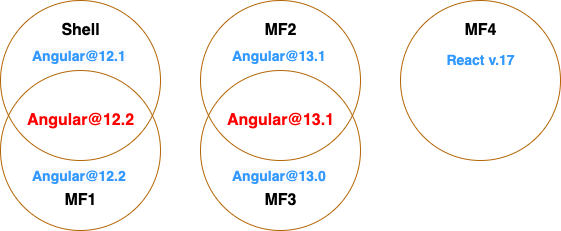
\includegraphics[width=0.7\textwidth]{Figures/multi_version_diagramm.drawio.png}
	\caption{WMF way of handling multi-versions}
	\label{fig:wmf_multiversions}
\end{figure}

As it can be seen, WMF always picks the latest major release, assuming the respective micro frontends have a similar configuration as shown in listing \ref{list:shared_mapping_wmf} applied. If, for instance, \textbf{MF3} has its \texttt{strictVersion} property set to \texttt{true}, it would cause the loading of its libraries too.

There are side effects to sharing the same dependency over the whole micro frontend landscape. One of which is the increase in bundle sizes, since every \textbf{remote} bundles its local dependencies. WMF then picks the one to serve during the runtime of the landscape.
This impact has a trade-off tough. Returning users can benefit from cached dependencies.\cite{wmf_multi_versions}

Integrating several \textbf{remotes} using the same dependencies leads to the issue of redundancies, which WMF is able to resolve. Via configuration of shared dependencies WMF provides a way to reduce redundant libraries in its landscape.
	% \glsresetall
\chapter{Presentation of the results} % Main chapter title
\label{Chapter6}

\lhead{Chapter 6. \emph{Presentation of the results}}

In this chapter it will be explained how empirical traffic data was gathered using the prototype and which metrics were defined for comparison.
Afterwards the landscapes will be compared, using the defined metrics as key performance indicators. The actual evaluation of the results will be concluded in chapter \ref{Chapter7}.

\section{Data collection and metric definition} 

This section will contain information about how the data was collected and which metrics were defined based on the gathered data.

\subsection{Data collection}

\subsubsection{Testing hardware and environment}

It has to be mentioned that certain aspects of the environment were not maintained by the tester and are therefore out of reach for influence or configuration. Nonetheless they are mentioned here for the sake of reproducibility.
The testing hardware and environment available were the following:

\begin{enumerate}
	\item \textbf{Laptop:}
	\begin{itemize}[noitemsep]
		\item MacBook Pro (15-inch, 2017)
		\item \textbf{Processor:} 2.9 GHz Quad-Core Intel Core i7
		\item \textbf{Memory:} 16 GB 2133 MHz LPDDR3 
		\item \textbf{Graphics:} Radeon Pro 560 4 GB and Intel HD Graphics 630 1536 MB
		\item \textbf{macOS Monetary - Version:} 12.2.1 (21D62)
	\end{itemize} 

	\item \textbf{Browser, Network and Lighthouse:}
	\begin{itemize}[noitemsep]
		\item \textbf{Browser:} Google Chrome
		\item \textbf{Version:} 99.0.4844.51 (Official Build) (x86\_64)
		\item \textbf{Chrome DevTools version:} Chrome 99
		\item \textbf{Lighthouse version:} 100.0.0.0
		\item \textbf{JavaScript version:} V8 9.9.115.8
		\item \textbf{Network-Bandwidth:} 180-200 MB/s
	\end{itemize}

	\item \textbf{Runtime environment for prototypes:} surge.sh \footnote{surge.sh is a platform for static web publishing
		for frontend developers via the command line.}
	
	\item \textbf{CDN:} Unpkg.com \footnote{This part of the environment was explained in chapter \ref{Chapter3}}
\end{enumerate}

Additionally to the specified hardware specs, version 1.18.1 of the \texttt{@luigi-project} was used. This dependency enables the Luigi framework and is therefore used in every implemented version of the prototype.

\subsubsection{Testing process}

Since multiple landscapes were implemented a unified process was required to collect comparable data. The BPMN diagram \ref{fig:data_collection_process_har} contains the process steps in detail.

\begin{figure}[!h]
	\centering
	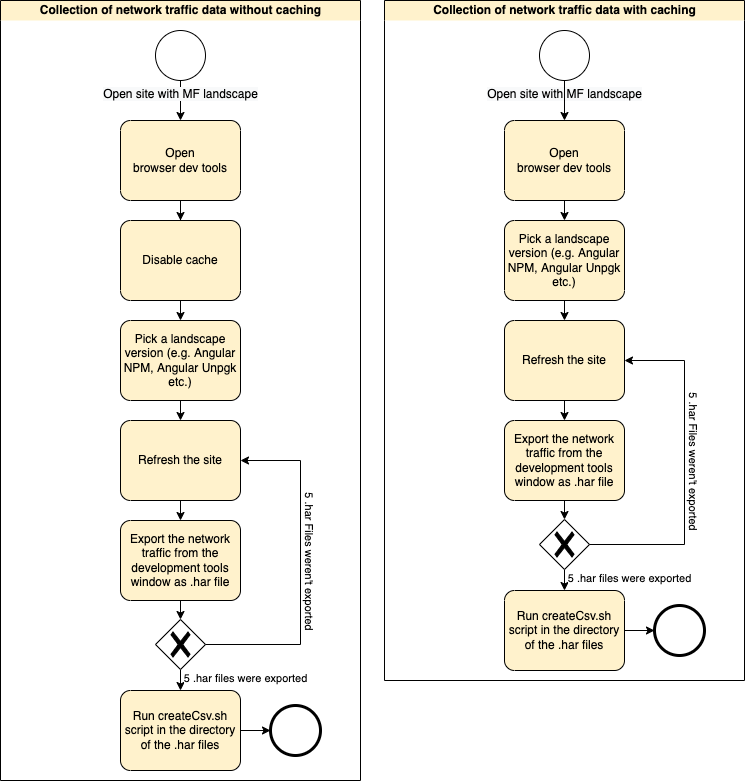
\includegraphics[width=0.7\textwidth]{Figures/Data_Collection_Process_har.drawio.png}
	\caption{Data collection process for .har files}
	\label{fig:data_collection_process_har}
\end{figure}

As it can be seen in \ref{fig:data_collection_process_har} there are actually two processes executed to collect data. The first one was with caching disabled, the second had it enabled. The intention behind it was to gather an average initial loading time for the picked side, therefore the resources must not be cached. 
The second process was used to gather information about caching behavior in general. Since each landscape contains basically the same views, the browser should be able to pull already loaded resources from the cache instead via the network. To showcase this behavior and prove the performance gain through caching, this data was gathered too.
Each process was executed 5 times, therefore 10 HTTP Archive (\texttt{.har}) files were generated per landscape. These \texttt{.har} files were then transformed into \texttt{.csv} files using a self-developed script. 

Additionally to the \texttt{.har} files a website performance report was collected, using the Lighthouse tool embedded in the Google Chrome browser. Such a report provides information about how much of the imported bytes are actually used by a web application, distinguished by resource URL.

After the collection process, another self-developed script was used to aggregate all the gather data into one single file. This was later used to define and calculate the metrics, which are described next.

\subsection{Defined metrics}

The central file, containing all the data, was split into separate sheets in which the metrics for each micro frontend were calculated. The parameters for calculation were:

\begin{itemize}
	\item \textbf{connection} - This is an ID with which each opened TCP connection is tagged by the browser. This value can be an indicator for the parallelity of the requests. Since HTTP/2 several requests can be handled by a server via the same TCP connection, reducing the time costs for TCP handshakes. It has to be considered that the application requesting the sources can not implement this HTTP/2 feature. It has to be enabled on server side and by the browser, which is already the case for most modern browsers.\cite{http2} As of writing this transcript, Surge the web server platform, onto which the application landscapes are deployed, does not support HTTP/2.
	
	\item \textbf{loadedFromCache} - This is a string value with three possible characteristics, \textit{not loaded from cache, disk} or \textit{memory}, whereas \textit{disk} and \textit{memory} are semantically the same. This value explains from where the resource was loaded. Either via the network from a remote server or from the local cache. It helps indicating the caching behavior of bundled resources in comparison with resources loaded from a unified URL (e.g. a CDN). 
	
	\item \textbf{pageRef} - This is a page reference provided by the browser with possibly an infinite amount of characteristics. Each request is tagged with this value, so it can be distinguished, which request was sent by which web application. Since the data is separated by sheets inside the file and is always website specific, no further information can be pulled from this value.
	
	\item \textbf{startedDateTime} - This is a time stamp given to each request, marking its starting time in a DateTime format. This value can serve as an indicator for parallelity, since multiple TCP connections can be opened at the same time. 
	
	\item \textbf{requestMethod} - This is a string value with a limited amount of characteristics. The possible values are the different HTTP methods. It indicates which type of request was executed for the loaded resource. In almost all cases it is \textbf{GET}.
	
	\item \textbf{requestUrl} - This is a string value, containing the request URL used by the browser to load the resource. This value is mainly categorizing the calculation results, since neither \textit{connection} nor \textit{pageRef} are valid options to distinguish the loaded resources of a website. 
	
	\item \textbf{requestHeaderSize} - This is a number value, indicating the byte size of the request header sent by the web application to the server.
	
	\item \textbf{responseStatus} - This is a number value with a limited amount of characteristics, containing the HTTP response code from the server. The range of the possible values is the same as the possible response codes of the HTTP.
	
	\item \textbf{responseContentSize} - This number value is the byte size of the loaded resource.
	
	\item \textbf{timeInMs} - This value represents the round trip time of the request in milliseconds. 
\end{itemize}

Based on the given values from the \texttt{.har} files, following key performance indicators were calculated.

\begin{itemize}
	\item \textbf{Avg. Content Size} - Numerical value calculated by averaging the \textbf{responseContentSize} values of all the websites resources
	\item \textbf{Avg. Time in MS Loaded values} - Numerical value, calculated by averaging the \textbf{timeInMs} values of all the websites resources
	\item \textbf{Occurrences Connection Duplicates} - Numerical value to represent parallelity by counting the amount of duplicate/multiple occurring \textbf{connection} values
	\item \textbf{Connection IDs} - List of all \textbf{connection} characteristics for the website 
	\item \textbf{Connection IDs occurrence} - Amount of how often the connection occurred during the loading of the website
	\item \textbf{Parallel start time} - Numerical value, calculated by counting reoccurring \textbf{startedDateTime} values
	\item \textbf{Avg. Response content size per Loading Type} - Numerical value, calculated by averaging the \textbf{responseContentSize}, differentiated by the characteristics of the \textbf{loadedFromCache} property
	\item \textbf{URLs loaded} - List of all unique \textbf{requestUrl} values
	\item \textbf{Avg. Response Time per URL loaded in MS} - Numerical value, representing the average loading time of each loaded resource URL of the website
	\item \textbf{Avg. Response Size per URL loaded} - Numerical value, representing the average loading byte size of each resource URL
	\item \textbf{Avg. Response Size per URL loaded via network} - Numerical value, calculated by averaging the \textbf{responseContentSize} differentiated by the \textbf{requestUrl} for all resources with the \textbf{loadedFromCache} value of \textit{not loaded from cache}. For the test scenarios with cache disabled, this value equals \textbf{Avg. Response Size per URL loaded}
	\item \textbf{Avg. Response Size per URL loaded from Disk} - Numerical value, calculated by averaging the \textbf{responseContentSize} differentiated by the \textbf{requestUrl}, for all resources with the \textbf{loadedFromCache} value of \textit{disk}
	\item \textbf{Avg. Response Size per URL loaded from Memory} - Numerical value, calculated by averaging the \textbf{responseContentSize} differentiated by the \textbf{requestUrl}, for all resources with the \textbf{loadedFromCache} value of \textit{memory}
\end{itemize}

The main focus of this thesis is to reduce redundant libraries in micro frontend landscapes, by using different types of technologies. Therefore, the calculated metrics were used to partially determine the gain a technology brings. Nonetheless, it has to be considered, that certain indicators are hard to measure such as the complexity of the implemented technology.  
A metric like this, must not be ignored for the context of this transcript, since the gain or rather the value a technology brings, highly depends on it. Thus a subjective retrospective will be provided in chapter \ref{Chapter7}, describing the experience of the author with the used technologies.

In the following sections the results of the introduced metrics for each landscape are showcased. This display is distinguished by the fact, if the collected data was with caching enabled or not. Additionally to the metrics, the individual graphs for the landscapes are referred to in the appendixes \ref{appendix1}, \ref{appendix2} and \ref{appendix3}.

\section{CDN landscapes}

\subsection{Implementation with NPM}

The table \ref{tab:cdn_result_table} contains the results for the implemented landscapes with a regular bundler and a package manager, namely NPM. Certain metrics are not added to the table for readability, but a graphical representation can be found in \ref{appendix1}.

\scriptsize 
\setlength{\mycolwidth}{\dimexpr \textwidth/5 - 2\tabcolsep}%

\begin{longtable}[l]{*{3}{p{\mycolwidth}}}
	
	\caption{Table of numerical KPI results for the NPM landscapes with caching disabled}
	\label{tab:cdn_result_table} \\
	
	\toprule
	\multicolumn{1}{l}{\makecell[c]{\textbf{Metric}}}   
	& \multicolumn{1}{l}{\makecell[c]{\textbf{Angular NPM}}}                              
	& \multicolumn{1}{l}{\makecell[c]{\textbf{Vue NPM}}} \\ 
	\midrule
	\endfirsthead
	
	\multicolumn{3}{l}{\footnotesize\itshape\tablename~\thetable:
		continued from previous page} \\
	\toprule   
	\multicolumn{1}{l}{\makecell[c]{\textbf{Metric}}}   
	& \multicolumn{1}{l}{\makecell[c]{\textbf{Angular NPM}}}                              
	& \multicolumn{1}{l}{\makecell[c]{\textbf{Vue NPM}}} \\*
	\midrule
	\endhead
	%		
	\multicolumn{1}{l|}{URLs loaded count}                                         															
	& \multicolumn{1}{l|}{\makecell[c]{14}} 	
	& \multicolumn{1}{l}{\makecell[c]{13}}   \\ \midrule
	
	\multicolumn{1}{l|}{\makecell[l]{Avg. Response content size\\per Loading Type}}   
	& \multicolumn{1}{l|}{\makecell[c]{\textit{not loaded from cache} - 129529.13, \\ \textit{memory} - 0, \\ \textit{disk} - 0}} 											
	& \multicolumn{1}{l}{\makecell[c]{\textit{not loaded from cache} - 156131.63, \\ \textit{memory} - 0, \\ \textit{disk} - 0}}   \\ \midrule
	
	\multicolumn{1}{l|}{Parallel start time}                                 													
	& \multicolumn{1}{l|}{\makecell[c]{33}} 				
	& \multicolumn{1}{l}{\makecell[c]{45}}   \\ \midrule
	
	\multicolumn{1}{l|}{Connection IDs occurence}                            											
	& \multicolumn{1}{l|}{\makecell[c]{\textit{none established} - 10,\\ \textit{207393} - 10}} 												   
	& \multicolumn{1}{l}{\makecell[c]{\textit{241394} - 10}}   \\ \midrule
	
	\multicolumn{1}{l|}{Connection IDs count}                                      																
	& \multicolumn{1}{l|}{\makecell[c]{62}} 															     
	& \multicolumn{1}{l}{\makecell[c]{71}}   \\ \midrule
		
	\multicolumn{1}{l|}{\makecell[l]{Connection Duplicates}}                        
	& \multicolumn{1}{l|}{\makecell[c]{20}} 						   
	& \multicolumn{1}{l}{\makecell[c]{10}}   \\ \midrule
	
	\multicolumn{1}{l|}{\makecell[l]{Loaded values \& occurrences}}                        
	& \multicolumn{1}{c|}{\makecell[c]{\textit{not loaded from cache} - 80,\\ \textit{memory} - 0, \\ \textit{disk} - 0}} 						   
	& \multicolumn{1}{l}{\makecell[c]{\textit{not loaded from cache} - 80, \\ \textit{memory} - 0, \\ \textit{disk} - 0}}   \\ \midrule
	
	\multicolumn{1}{l|}{\makecell[l]{Avg. Time in MS}}                        
	& \multicolumn{1}{l|}{\makecell[c]{162.22}} 						   
	& \multicolumn{1}{l}{\makecell[c]{5323.54}}   \\ \midrule
	
	\multicolumn{1}{l|}{\makecell[l]{Avg. Content Size}}                                         
	& \multicolumn{1}{l|}{\makecell[c]{129529.13}}  				  
	&   \multicolumn{1}{l}{\makecell[c]{156131.63}} \\ \bottomrule
\end{longtable}

The results shown in table \ref{tab:cdn_result_table} were collected without caching enabled. This explains for instance, why no resources were loaded from cache and therefore the values for the \textit{memory} or \textit{disk} characteristics are missing.
The main takeaway from these results, is an average initial loading time for the landscapes which range from \textbf{129529.125} to \textbf{156131.625} milliseconds, depending on the framework. It can also be seen, that even though less resources are loaded via URLs by the VueJS landscape, it has a longer loading time compared to the Angular one.

\begin{longtable}[l]{*{3}{p{\mycolwidth}}}
	
	\caption{Table of numerical KPI results for the NPM landscapes with caching enabled}
	\label{tab:cdn_result_table_caching} \\
	
	\toprule
	\multicolumn{1}{l}{\makecell[c]{\textbf{Metric}}}   
	& \multicolumn{1}{l}{\makecell[c]{\textbf{Angular NPM}}}                              
	& \multicolumn{1}{l}{\makecell[c]{\textbf{Vue NPM}}} \\ 
	\midrule
	\endfirsthead
	
	\multicolumn{3}{l}{\footnotesize\itshape\tablename~\thetable:
		continued from previous page} \\
	\toprule   
	\multicolumn{1}{l}{\makecell[c]{\textbf{Metric}}}   
	& \multicolumn{1}{l}{\makecell[c]{\textbf{Angular NPM}}}                              
	& \multicolumn{1}{l}{\makecell[c]{\textbf{Vue NPM}}} \\*
	\midrule
	\endhead
	%		
	\multicolumn{1}{l|}{URLs loaded count}                                         															
	& \multicolumn{1}{l|}{\makecell[c]{14}} 	
	& \multicolumn{1}{l}{\makecell[c]{13}}   \\ \midrule
	
	\multicolumn{1}{l|}{\makecell[l]{Avg. Response content size\\per Loading Type}}   
	& \multicolumn{1}{l|}{\makecell[c]{\textit{not loaded from cache} - 166856, \\ \textit{memory} - 17548.5, \\ \textit{disk} - 17548.5}} 											
	& \multicolumn{1}{l}{\makecell[c]{\textit{not loaded from cache} - 145646.67,\\ \textit{memory} - 0, \\ \textit{disk} - 187586.5}}   \\ \midrule
	
	\multicolumn{1}{l|}{Parallel start time}                                 													
	& \multicolumn{1}{l|}{\makecell[c]{32}} 				
	& \multicolumn{1}{l}{\makecell[c]{39}}   \\ \midrule
	
	\multicolumn{1}{l|}{Connection IDs occurence}                            											
	& \multicolumn{1}{l|}{\makecell[c]{\textit{none established} - 20}} 												   
	& \multicolumn{1}{l}{\makecell[c]{\textit{none established} - 20}}   \\ \midrule
	
	\multicolumn{1}{l|}{Connection IDs count}                                      																
	& \multicolumn{1}{l|}{\makecell[c]{61}} 															     
	& \multicolumn{1}{l}{\makecell[c]{61}}   \\ \midrule
	
	\multicolumn{1}{l|}{\makecell[l]{Connection Duplicates}}                        
	& \multicolumn{1}{l|}{\makecell[c]{20}} 						   
	& \multicolumn{1}{l}{\makecell[c]{20}}   \\ \midrule
	
	\multicolumn{1}{l|}{\makecell[l]{Loaded values \& occurrences}}                        
	& \multicolumn{1}{c|}{\makecell[c]{\textit{not loaded from cache} - 60, \\ \textit{memory} - 6, \\ \textit{disk} - 14}} 						   
	& \multicolumn{1}{l}{\makecell[c]{\textit{not loaded from cache} - 60, \\ \textit{memory} - 0, \\ \textit{disk} - 20}}   \\ \midrule
	
	\multicolumn{1}{l|}{\makecell[l]{Avg. Time in MS}}                        
	& \multicolumn{1}{l|}{\makecell[c]{150.90}} 						   
	& \multicolumn{1}{l}{\makecell[c]{1890.6}}   \\ \midrule
	
	\multicolumn{1}{l|}{\makecell[l]{Avg. Content Size}}                                         
	& \multicolumn{1}{l|}{\makecell[c]{129529.13}}  				  
	&   \multicolumn{1}{l}{\makecell[c]{156131.63}} \\ \bottomrule
	
\end{longtable}

The results of table \ref{tab:cdn_result_table_caching} show the effect caching has on the performance of a site. The average loading time of the site decreases, as do the opened TCP connections. In table \ref{cdn_result_table}, the Angular landscape is loaded faster compared to Vue JS.

Both environments were implemented using a regular bundler and therefore it can not be ensured that redundant libraries were not loaded.

\subsection{Implementation with Unpkg}

Table \ref{tab:cdn_result_table_unpkg} contains the results for the implemented landscapes with a use of a public CDN, namely Unpkg. Certain metrics are not added to the table for readability, but a graphical representation can be found in \ref{appendix1}. 

\begin{longtable}[c]{*{3}{p{\mycolwidth}}}
	
	\caption{Table of numerical KPI results for the landscapes using the Unpkg CDN with caching disabled}
	\label{tab:cdn_result_table_unpkg} \\
	
	\toprule
	\multicolumn{1}{l}{\makecell[c]{\textbf{Metric}}}   
	& \multicolumn{1}{l}{\makecell[c]{\textbf{Angular Unpkg}}}                              
	& \multicolumn{1}{l}{\makecell[c]{\textbf{Vue Unpkg}}} \\ 
	\midrule
	\endfirsthead
	
	\multicolumn{3}{l}{\footnotesize\itshape\tablename~\thetable:
		continued from previous page} \\
	\toprule                        
	\multicolumn{1}{l}{\makecell[c]{\textbf{Metric}}}   
	& \multicolumn{1}{l}{\makecell[c]{\textbf{Angular Unpkg}}}                              
	& \multicolumn{1}{l}{\makecell[c]{\textbf{Vue Unpkg}}} \\*
	\midrule
	\endhead
	%		
	\multicolumn{1}{l|}{URLs loaded count}                                         															
	& \multicolumn{1}{l|}{\makecell[c]{171}} 	
	& \multicolumn{1}{l}{\makecell[c]{165}}   \\ \midrule
	
	\multicolumn{1}{l|}{\makecell[l]{Avg. Response content size\\per Loading Type}}   
	& \multicolumn{1}{l|}{\makecell[c]{\textit{not loaded from cache} - 9768.62, \\ \textit{memory} - 0, \\ \textit{disk} - 0}} 											
	& \multicolumn{1}{l}{\makecell[c]{\textit{not loaded from cache} - 8205.19, \\ \textit{memory} - 0, \\ \textit{disk} - 0}}   \\ \midrule
	
	\multicolumn{1}{l|}{Parallel start time}                                 													
	& \multicolumn{1}{l|}{\makecell[c]{871}} 				
	& \multicolumn{1}{l}{\makecell[c]{989}}   \\ \midrule
	
	\multicolumn{1}{l|}{Connection IDs occurence}                            											
	& \multicolumn{1}{l|}{\makecell[c]{\textit{223736} - 20,\\ \textit{223722} - 1574,\\ \textit{none established} - 10}} 												   
	& \multicolumn{1}{l}{\makecell[c]{\textit{241394} - 20,\\ \textit{249654} - 1560}}   \\ \midrule
	
	\multicolumn{1}{l|}{Connection IDs count}                                      																
	& \multicolumn{1}{l|}{\makecell[c]{53}} 															     
	& \multicolumn{1}{l}{\makecell[c]{42}}   \\ \midrule
	
	\multicolumn{1}{l|}{\makecell[l]{Connection Duplicates}}                        
	& \multicolumn{1}{l|}{\makecell[c]{1604}} 						   
	& \multicolumn{1}{l}{\makecell[c]{1580}}   \\ \midrule
	
	\multicolumn{1}{l|}{\makecell[l]{Loaded values \&\\ occurrences}}                        
	& \multicolumn{1}{c|}{\makecell[c]{\textit{not loaded from cache} - 1654, \\ \textit{memory} - 0, \\ \textit{disk} - 0}} 						   
	& \multicolumn{1}{l}{\makecell[c]{\textit{not loaded from cache} - 1620, \\ \textit{memory} - 0, \\ \textit{disk} - 0}}   \\ \midrule
	
	\multicolumn{1}{l|}{\makecell[l]{Avg. Time in MS}}                        
	& \multicolumn{1}{l|}{\makecell[c]{97.23}} 						   
	& \multicolumn{1}{l}{\makecell[c]{194.01}}   \\ \midrule
	
	\multicolumn{1}{l|}{\makecell[l]{Avg. Content Size}}                                         
	& \multicolumn{1}{l|}{\makecell[c]{9768.62}}  				  
	&   \multicolumn{1}{l}{\makecell[c]{8205.19}} \\ \bottomrule
	
\end{longtable}

 The data shown in table \ref{tab:cdn_result_table_unpkg} are again collected without caching enabled. An approximate estimation for the initial loading times can be drawn from this. It is made visible that the VueJS environment takes longer to load for less content. A similar behavior was present in the NPM implementation.
 Nonetheless it is an improvement in performance compared to the NPM counterparts for both landscapes. The trade-off of this technology is that single component resources, like a button or a table, were imported via script tags one by one, thus the increase in loaded URLs.
  
\begin{longtable}[c]{*{3}{p{\mycolwidth}}}
 	
 	\caption{Table of numerical KPI results for the landscapes using the Unpkg CDN with caching enabled}
 	\label{tab:cdn_result_table_unpkg_cache} \\
 	
 	\toprule
	\multicolumn{1}{l}{\makecell[c]{\textbf{Metric}}}   
	& \multicolumn{1}{l}{\makecell[c]{\textbf{Angular Unpkg}}}                              
	& \multicolumn{1}{l}{\makecell[c]{\textbf{Vue Unpkg}}} \\ 
 	\midrule
 	\endfirsthead
 	
 	\multicolumn{3}{l}{\footnotesize\itshape\tablename~\thetable:
 		continued from previous page} \\
 	\toprule   
	\multicolumn{1}{l}{\makecell[c]{\textbf{Metric}}}   
	& \multicolumn{1}{l}{\makecell[c]{\textbf{Angular Unpkg}}}                              
	& \multicolumn{1}{l}{\makecell[c]{\textbf{Vue Unpkg}}} \\*
 	\midrule
 	\endhead
 	%		
 	\multicolumn{1}{l|}{URLs loaded count}                                         															
 	& \multicolumn{1}{l|}{\makecell[c]{171}} 	
 	& \multicolumn{1}{l}{\makecell[c]{165}}   \\ \midrule
 	
 	\multicolumn{1}{l|}{\makecell[l]{Avg. Response content size\\per Loading Type}}   
 	& \multicolumn{1}{l|}{\makecell[c]{\textit{not loaded from cache} - 63972.08, \\ \textit{memory} - 208838, \\ \textit{disk} - 7166.1}} 											
 	& \multicolumn{1}{l}{\makecell[c]{\textit{not loaded from cache} - 28143.2, \\ \textit{memory} - 0, \\ \textit{disk} - 7570.22}}   \\ \midrule
 	
 	\multicolumn{1}{l|}{Parallel start time}                                 													
 	& \multicolumn{1}{l|}{\makecell[c]{1111}} 				
 	& \multicolumn{1}{l}{\makecell[c]{1069}}   \\ \midrule
 	
 	\multicolumn{1}{l|}{Connection IDs occurence}                            											
 	& \multicolumn{1}{l|}{\makecell[c]{\textit{none established} - 1590,\\ \textit{223722} - 15}} 												   
 	& \multicolumn{1}{l}{\makecell[c]{\textit{none established} - 1570,\\ \textit{249654} - 10}}   \\ \midrule
 	
 	\multicolumn{1}{l|}{Connection IDs count}                                      																
 	& \multicolumn{1}{l|}{\makecell[c]{52}} 															     
 	& \multicolumn{1}{l}{\makecell[c]{42}}   \\ \midrule
 	
 	\multicolumn{1}{l|}{\makecell[l]{Connection Duplicates}}                        
 	& \multicolumn{1}{l|}{\makecell[c]{1605}} 						   
 	& \multicolumn{1}{l}{\makecell[c]{1580}}   \\ \midrule
 	
 	\multicolumn{1}{l|}{\makecell[l]{Loaded values \& occurrences}}                        
 	& \multicolumn{1}{c|}{\makecell[c]{\textit{not loaded from cache} - 65, \\ \textit{memory} - 3, \\ \textit{disk} - 1587}} 						   
 	& \multicolumn{1}{l}{\makecell[c]{\textit{not loaded from cache} - 50, \\ \textit{memory} - 0, \\ \textit{disk} - 1570}}   \\ \midrule
 	
 	\multicolumn{1}{l|}{\makecell[l]{Avg. Time in MS}}                        
 	& \multicolumn{1}{l|}{\makecell[c]{58.73}} 						   
 	& \multicolumn{1}{l}{\makecell[c]{87.1}}   \\ \midrule
 	
 	\multicolumn{1}{l|}{\makecell[l]{Avg. Content Size}}                                         
 	& \multicolumn{1}{l|}{\makecell[c]{9762.72}}  				  
 	&   \multicolumn{1}{l}{\makecell[c]{8205.19}} \\ \bottomrule
 	
\end{longtable}

A similar development can be observed in table \ref{tab:cdn_result_table_unpkg_cache} as previously. Primarily with caching enabled, the average loading times decrease, secondly the amount of loaded resources from cache increases significantly and lastly the Angular environments show shorter average loading times despite more resources were requested by them.

\section{Web Components/Compound and WMF landscapes}

As the described in chapter \ref{Chapter4}, these environments exist in different versions. They were designed that way to showcase how the used technologies handle multi-version landscapes and how they affect the performance.
Table \ref{tab:wmf_compound} shows the above mentioned KPIs of those environments.
 
\begin{longtable}[c]{*{3}{p{\mycolwidth}}}
	
	\caption{Table of numerical KPI results for the landscapes implemented with Web Components as Compound Views and WMF with caching disabled}
	\label{tab:wmf_compound} \\
	
	\toprule
	\multicolumn{1}{l}{\makecell[c]{\textbf{Metric}}}   
	& \multicolumn{1}{l}{\makecell[c]{\textbf{WC/Compound }}}                              
	& \multicolumn{1}{l}{\makecell[c]{\textbf{WMF}}} \\ 
	\midrule
	\endfirsthead
	
	\multicolumn{3}{l}{\footnotesize\itshape\tablename~\thetable: continued from previous page} \\
	\toprule                        
	\multicolumn{1}{l}{\makecell[c]{\textbf{Metric}}}   
	& \multicolumn{1}{l}{\makecell[c]{\textbf{WC/Compound }}}                              
	& \multicolumn{1}{l}{\makecell[c]{\textbf{WMF}}} \\*
	\midrule
	\endhead
	%		
	\multicolumn{1}{l|}{URLs loaded count}                                         															
	& \multicolumn{1}{l|}{\makecell[c]{27}} 	       
	& \multicolumn{1}{l}{\makecell[c]{118}}   \\ \midrule
	
	\multicolumn{1}{l|}{\makecell[l]{Avg. Response content size\\per Loading Type}}   
	& \multicolumn{1}{l|}{\makecell[c]{\textit{not loaded from cache} - 213266.74, \\ \textit{memory} - 0,\\ \textit{disk} - 0}} 			         
	& \multicolumn{1}{l}{\makecell[c]{\textit{not loaded from cache} - 507168.76, \\ \textit{memory} - 0, \\ \textit{disk} - 0}}   \\ \midrule
	
	\multicolumn{1}{l|}{Parallel start time}                                 													
	& \multicolumn{1}{l|}{\makecell[c]{29}} 				                  
	& \multicolumn{1}{l}{\makecell[c]{109}}   \\ \midrule
	
	\multicolumn{1}{l|}{Connection IDs occurence}                            											
	& \multicolumn{1}{l|}{\makecell[c]{\textit{78725} - 15,\\ \textit{78890} - 15}} 		              
	& \multicolumn{1}{l}{\makecell[c]{\textit{728247} - 3,\\ \textit{none established} - 14}}   \\ \midrule
	
	\multicolumn{1}{l|}{Connection IDs count}                                      																
	& \multicolumn{1}{l|}{\makecell[c]{546}} 		         											     
	& \multicolumn{1}{l}{\makecell[c]{42}}   \\ \midrule
	
	\multicolumn{1}{l|}{\makecell[l]{Connection Duplicates}}                        
	& \multicolumn{1}{l|}{\makecell[c]{30}} 					
	& \multicolumn{1}{l}{\makecell[c]{20}}   \\ \midrule
	
	\multicolumn{1}{l|}{\makecell[l]{Loaded values \& occurrences}}                          
	& \multicolumn{1}{c|}{\makecell[c]{\textit{not loaded from cache} - 135, \\ \textit{memory} - 30, \\ \textit{disk} - 0}} 						   
	& \multicolumn{1}{l}{\makecell[c]{\textit{not loaded from cache} - 563, \\ \textit{memory} - 0, \\ \textit{disk} - 0}}   \\ \midrule
	
	\multicolumn{1}{l|}{\makecell[l]{Avg. Time in MS}}                        
	& \multicolumn{1}{l|}{\makecell[c]{2454.95}} 	                			   
	& \multicolumn{1}{l}{\makecell[c]{552.7}}   \\ \midrule
	
	\multicolumn{1}{l|}{\makecell[l]{Avg. Content Size}}                                         
	& \multicolumn{1}{l|}{\makecell[c]{213266.74}}  		          
	&   \multicolumn{1}{l}{\makecell[c]{507168.76}} \\ \bottomrule
	
\end{longtable}

As the data in table \ref{tab:wmf_compound} shows, the initial loading time for the Compound/Web Components environments is significantly lower compared to the WMF counterpart. Also the amount of loaded resources differs. This is due to the fact, that WMF has to be used in combination with the Webpack 5 bundler. Therefore certain resources might be loaded several times, if not configured as shared dependencies in the Module Federation. 
Table \ref{tab:wmf_compound_cache} showcases the same landscapes, but with caching enabled.

\begin{longtable}[c]{*{3}{p{\mycolwidth}}}
	
	\caption{Table of numerical KPI results for the landscapes implemented with Web Components as Compound Views and WMF with caching enabled}
	\label{tab:wmf_compound_cache} \\
	
	\toprule
	\multicolumn{1}{l}{\makecell[c]{\textbf{Metric}}}   
	& \multicolumn{1}{l}{\makecell[c]{\textbf{WC/Compound }}}                              
	& \multicolumn{1}{l}{\makecell[c]{\textbf{WMF}}} \\ 
	\midrule
	\endfirsthead
	
	\multicolumn{3}{l}{\footnotesize\itshape\tablename~\thetable: continued from previous page} \\
	\toprule                        
	\multicolumn{1}{l}{\makecell[c]{\textbf{Metric}}}   
	& \multicolumn{1}{l}{\makecell[c]{\textbf{WC/Compound }}}                              
	& \multicolumn{1}{l}{\makecell[c]{\textbf{WMF}}} \\*
	\midrule
	\endhead
	%		
	\multicolumn{1}{l|}{URLs loaded count}                                         															
	& \multicolumn{1}{l|}{\makecell[c]{27}} 	       
	& \multicolumn{1}{l}{\makecell[c]{109}}   \\ \midrule
	
	\multicolumn{1}{l|}{\makecell[l]{Avg. Response content size\\per Loading Type}}   
	& \multicolumn{1}{l|}{\makecell[c]{\textit{not loaded from cache} - 215385.36, \\ \textit{memory} - 167973, \\ \textit{disk} - 588082}} 			         
	& \multicolumn{1}{l}{\makecell[c]{\textit{not loaded from cache} - 525243.08, \\ \textit{memory} - 0, \\ \textit{disk} - 1959}}   \\ \midrule
	
	\multicolumn{1}{l|}{Parallel start time}                                 													
	& \multicolumn{1}{l|}{\makecell[c]{35}} 				                  
	& \multicolumn{1}{l}{\makecell[c]{105}}   \\ \midrule
	
	\multicolumn{1}{l|}{Connection IDs occurence}                            											
	& \multicolumn{1}{l|}{\makecell[c]{\textit{none established} - 4,\\ \textit{78890} - 15,\\ \textit{78725} - 11}} 		              
	& \multicolumn{1}{l}{\makecell[c]{\textit{none established} - 15}}   \\ \midrule
	
	\multicolumn{1}{l|}{Connection IDs count}                                      																
	& \multicolumn{1}{l|}{\makecell[c]{104}} 		         											     
	& \multicolumn{1}{l}{\makecell[c]{537}}   \\ \midrule
	
	\multicolumn{1}{l|}{\makecell[l]{Connection Duplicates}}                        
	& \multicolumn{1}{l|}{\makecell[c]{30}} 					
	& \multicolumn{1}{l}{\makecell[c]{15}}   \\ \midrule
	
	\multicolumn{1}{l|}{\makecell[l]{Loaded values \& occurrences}}                          
	& \multicolumn{1}{c|}{\makecell[c]{\textit{not loaded from cache} - 107, \\ \textit{memory} - 20, \\ \textit{disk} - 4}} 						   
	& \multicolumn{1}{l}{\makecell[c]{\textit{not loaded from cache} - 536, \\ \textit{memory} - 0, \\ \textit{disk} - 15}}   \\ \midrule
	
	\multicolumn{1}{l|}{\makecell[l]{Avg. Time in MS}}                        
	& \multicolumn{1}{l|}{\makecell[c]{897.62}} 	                			   
	& \multicolumn{1}{l}{\makecell[c]{356.53}}   \\ \midrule
	
	\multicolumn{1}{l|}{\makecell[l]{Avg. Content Size}}                                         
	& \multicolumn{1}{l|}{\makecell[c]{219526.89}}  		          
	&   \multicolumn{1}{l}{\makecell[c]{510997.6}} \\ \bottomrule
	
\end{longtable}

The results with the caching enabled are not so different compared to the disabled caching ones. For instances, in both cases the average loading time for the Compound landscape has longer loading times for fewer resources. One aspect differs though, compared to the Compound landscape the WMF one has little cached resources. Also it becomes visible that the average content size loaded is smaller. Therefore, the Lighthouse tool was used to gather further information and data about those applications. The next section will showcase and explain the analysis done.

\section{Lighthouse analysis}

It has to be mentioned in advance that the following data is considered to be representative. Therefore, it is assumed that similar landscapes would follow a similar result in general. Nonetheless it is possible that for single cases the reports differ, since the within lying calculations are highly application dependent.
For the sake of completeness the reports are shown below.

The given data was gathered based on the previously introduced landscapes. It contains the analysis of the imported resources and how much of the corresponding imports were not used by the application, measured in bytes. First a tabular view is provided, following by the corresponding graph.

\scriptsize 
\setlength{\mycolwidthtwo}{\dimexpr \textwidth/5 - 2\tabcolsep}%

\begin{longtable}[c]{*{4}{p{\mycolwidthtwo}}}
	
	\caption{Table of the average imported and unused bytes values, collected via the Lighthouse tool in the prototype landscapes}
	\label{tab:lighthouse_used_report} \\
	
	\toprule
	\textbf{Landscape}                        
	& \multicolumn{1}{l}{\makecell[c]{\textbf{Avg. imported bytes}}}   
	& \multicolumn{1}{l}{\makecell[c]{\textbf{Avg. unused bytes}}}                              
	& \multicolumn{1}{l}{\makecell[c]{\textbf{Avg. unused bytes in \%}}} \\                                    
	\midrule
	\endfirsthead
	
	\multicolumn{4}{l}{\footnotesize\itshape\tablename~\thetable: continued from previous page} \\
	\toprule        
	\textbf{Landscape}                        
	& \multicolumn{1}{l}{\makecell[c]{\textbf{Avg. imported bytes}}}   
	& \multicolumn{1}{l}{\makecell[c]{\textbf{Avg. unused bytes}}}                              
	& \multicolumn{1}{l}{\makecell[c]{\textbf{Avg. unused bytes in \%}}} \\*
	\midrule
	\endhead
	%		
	\multicolumn{1}{l|}{Angular NPM}                                         															
	& \multicolumn{1}{l|}{\makecell[c]{219257.14}} 	       
	& \multicolumn{1}{l|}{\makecell[c]{93671.43}}   
	& \multicolumn{1}{l}{\makecell[c]{42.72}} 	\\ \midrule
		
	\multicolumn{1}{l|}{Angular Unpkg}                                 													
	& \multicolumn{1}{l|}{\makecell[c]{13126.84}} 				                  
	& \multicolumn{1}{l|}{\makecell[c]{7425.87}}   
	& \multicolumn{1}{l}{\makecell[c]{56.57}} \\ \midrule
	
	\multicolumn{1}{l|}{Vue NPM}                            											
	& \multicolumn{1}{l|}{\makecell[c]{281262.33}} 		              
	& \multicolumn{1}{l|}{\makecell[c]{123902}}    
	& \multicolumn{1}{l}{\makecell[c]{44.05}} \\ \midrule
	
	\multicolumn{1}{l|}{Vue Unpkg}                                      																
	& \multicolumn{1}{l|}{\makecell[c]{12057.91}} 		         											     
	& \multicolumn{1}{l|}{\makecell[c]{6844.21}}    
	& \multicolumn{1}{l}{\makecell[c]{56.76}} \\ \midrule
	
	\multicolumn{1}{l|}{\makecell[l]{Compound/\\Web Components}}                        
	& \multicolumn{1}{l|}{\makecell[c]{229483.67}} 					
	& \multicolumn{1}{l|}{\makecell[c]{90265.19}}    
	& \multicolumn{1}{l}{\makecell[c]{39.33}} \\ \midrule
	
	\multicolumn{1}{l|}{\makecell[l]{Webpack\\Module\\Federation}}                         
	& \multicolumn{1}{l|}{\makecell[c]{551111.19}} 						   
	& \multicolumn{1}{l|}{\makecell[c]{222113.73}}   
	& \multicolumn{1}{l}{\makecell[c]{40.31}}  \\ \midrule
\end{longtable}

\begin{figure}[!h]
	\centering
	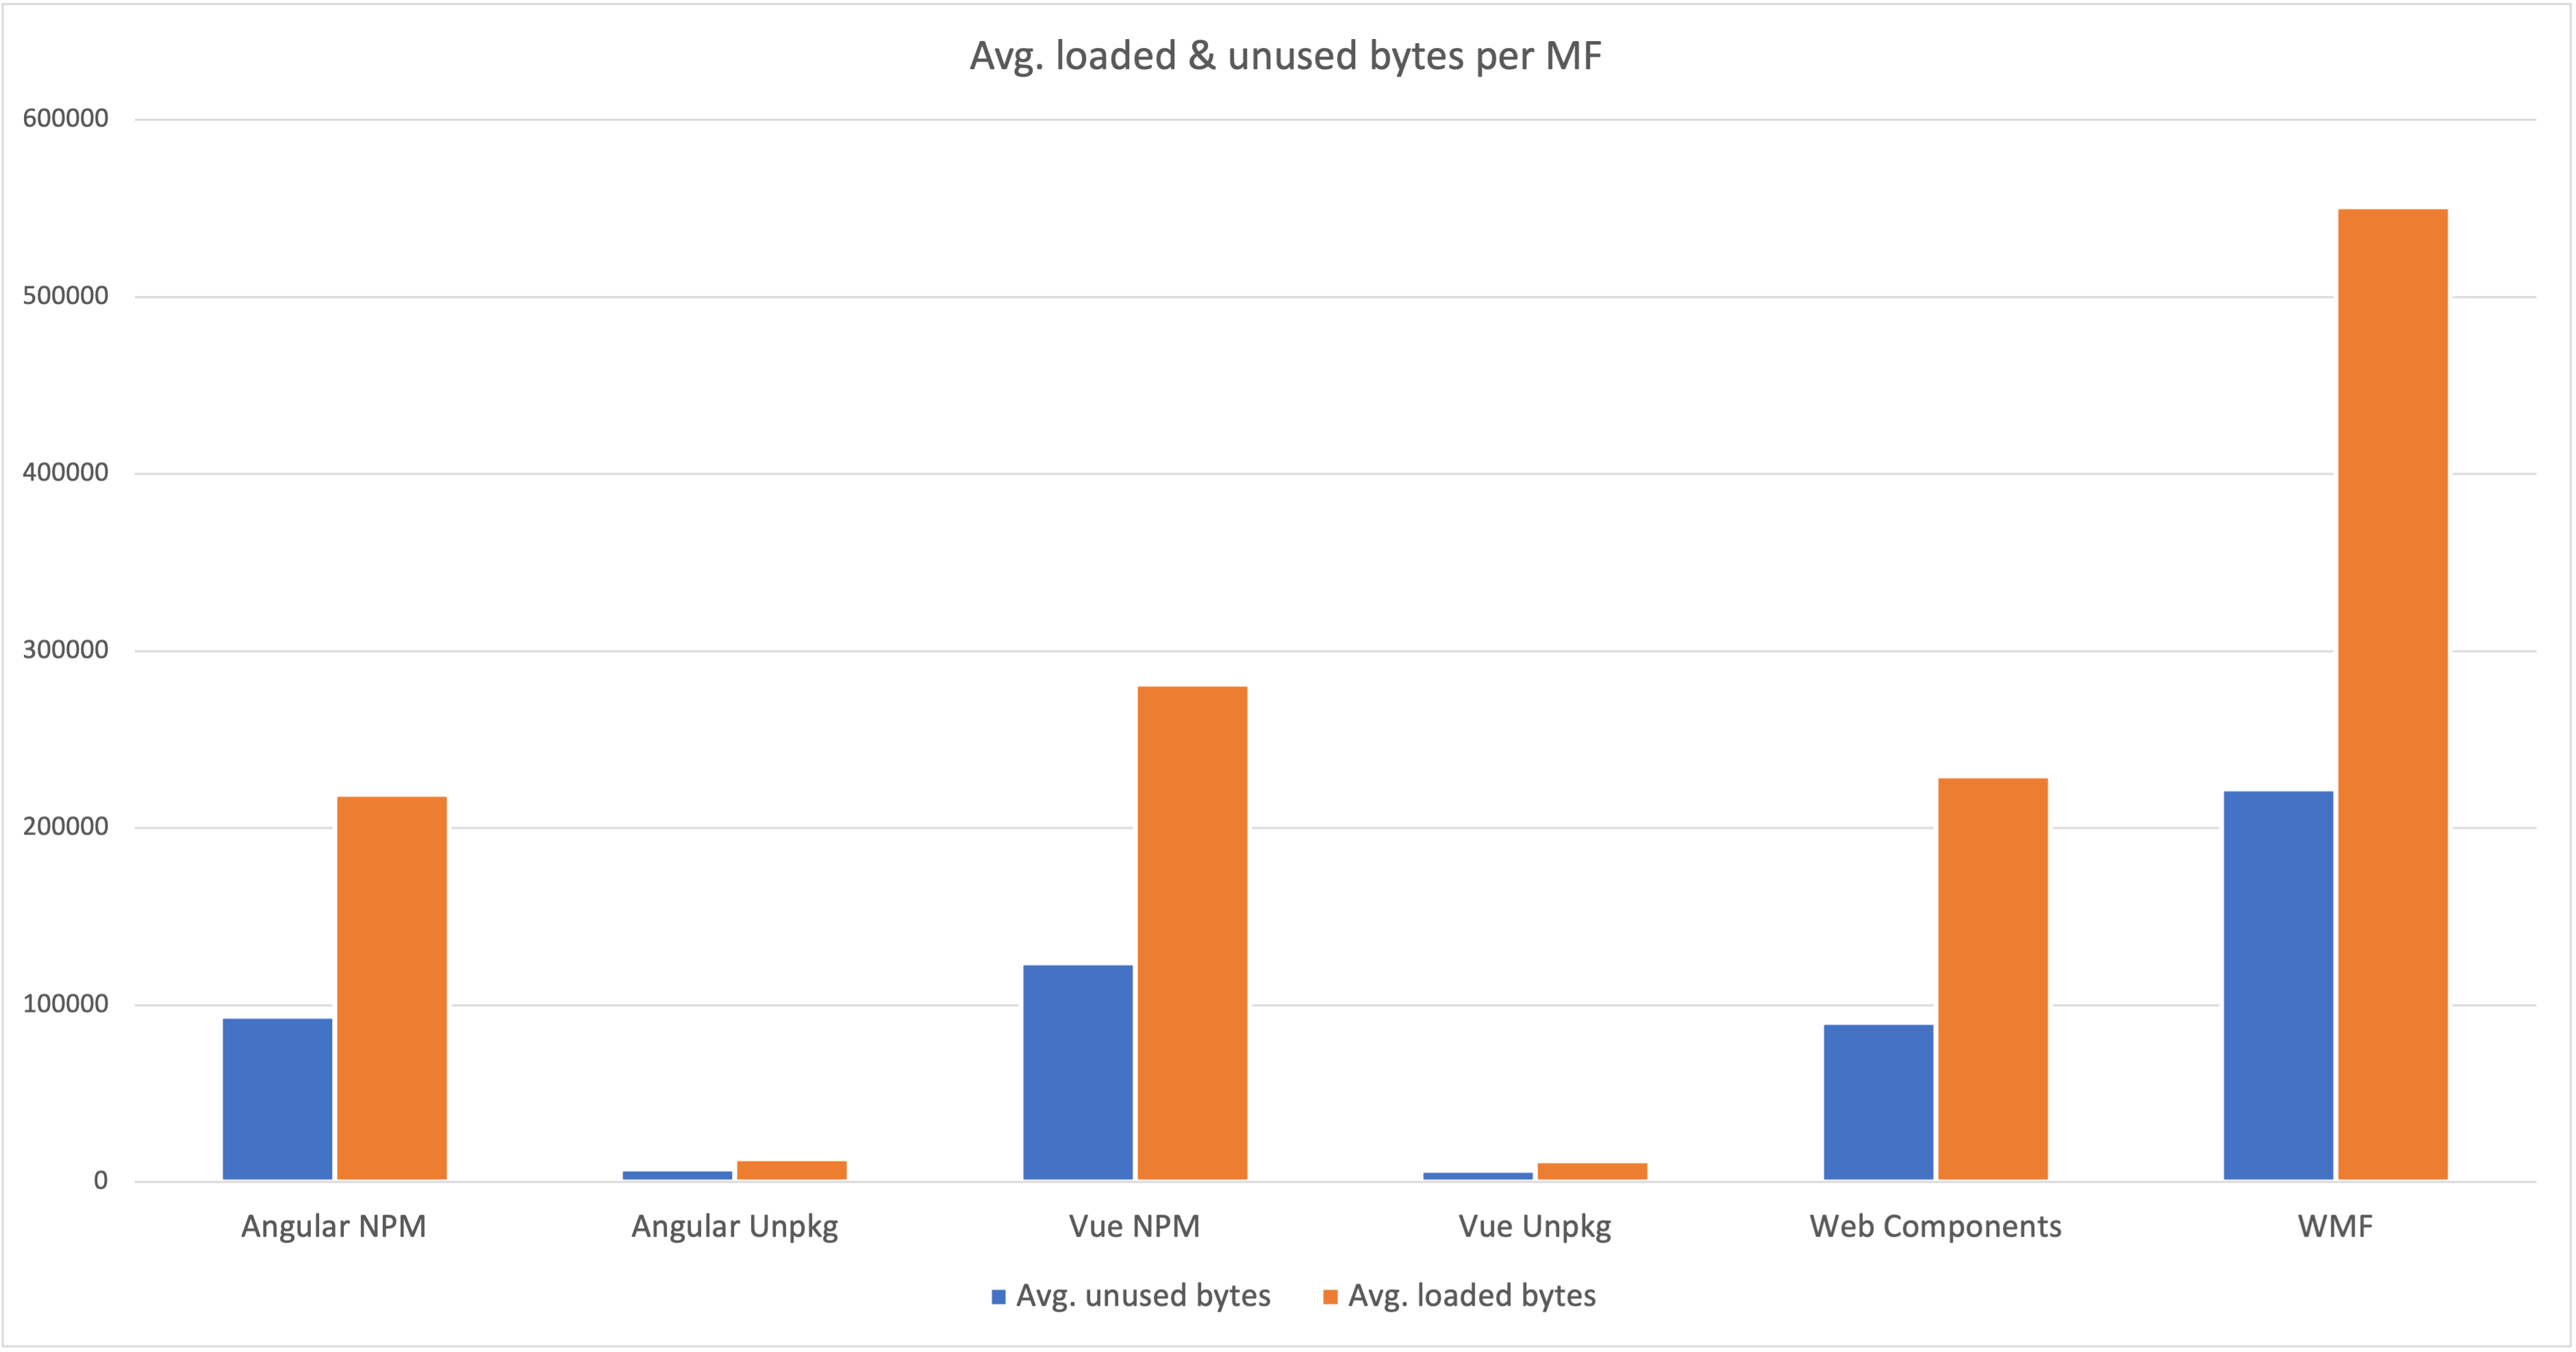
\includegraphics[width=1\textwidth]{Figures/avg_unsed_imported_1.png}
	\caption{Unused and imported bytes per landscape}
	\label{fig:unsed_imported_1}
\end{figure}

\begin{figure}[!h]
	\centering
	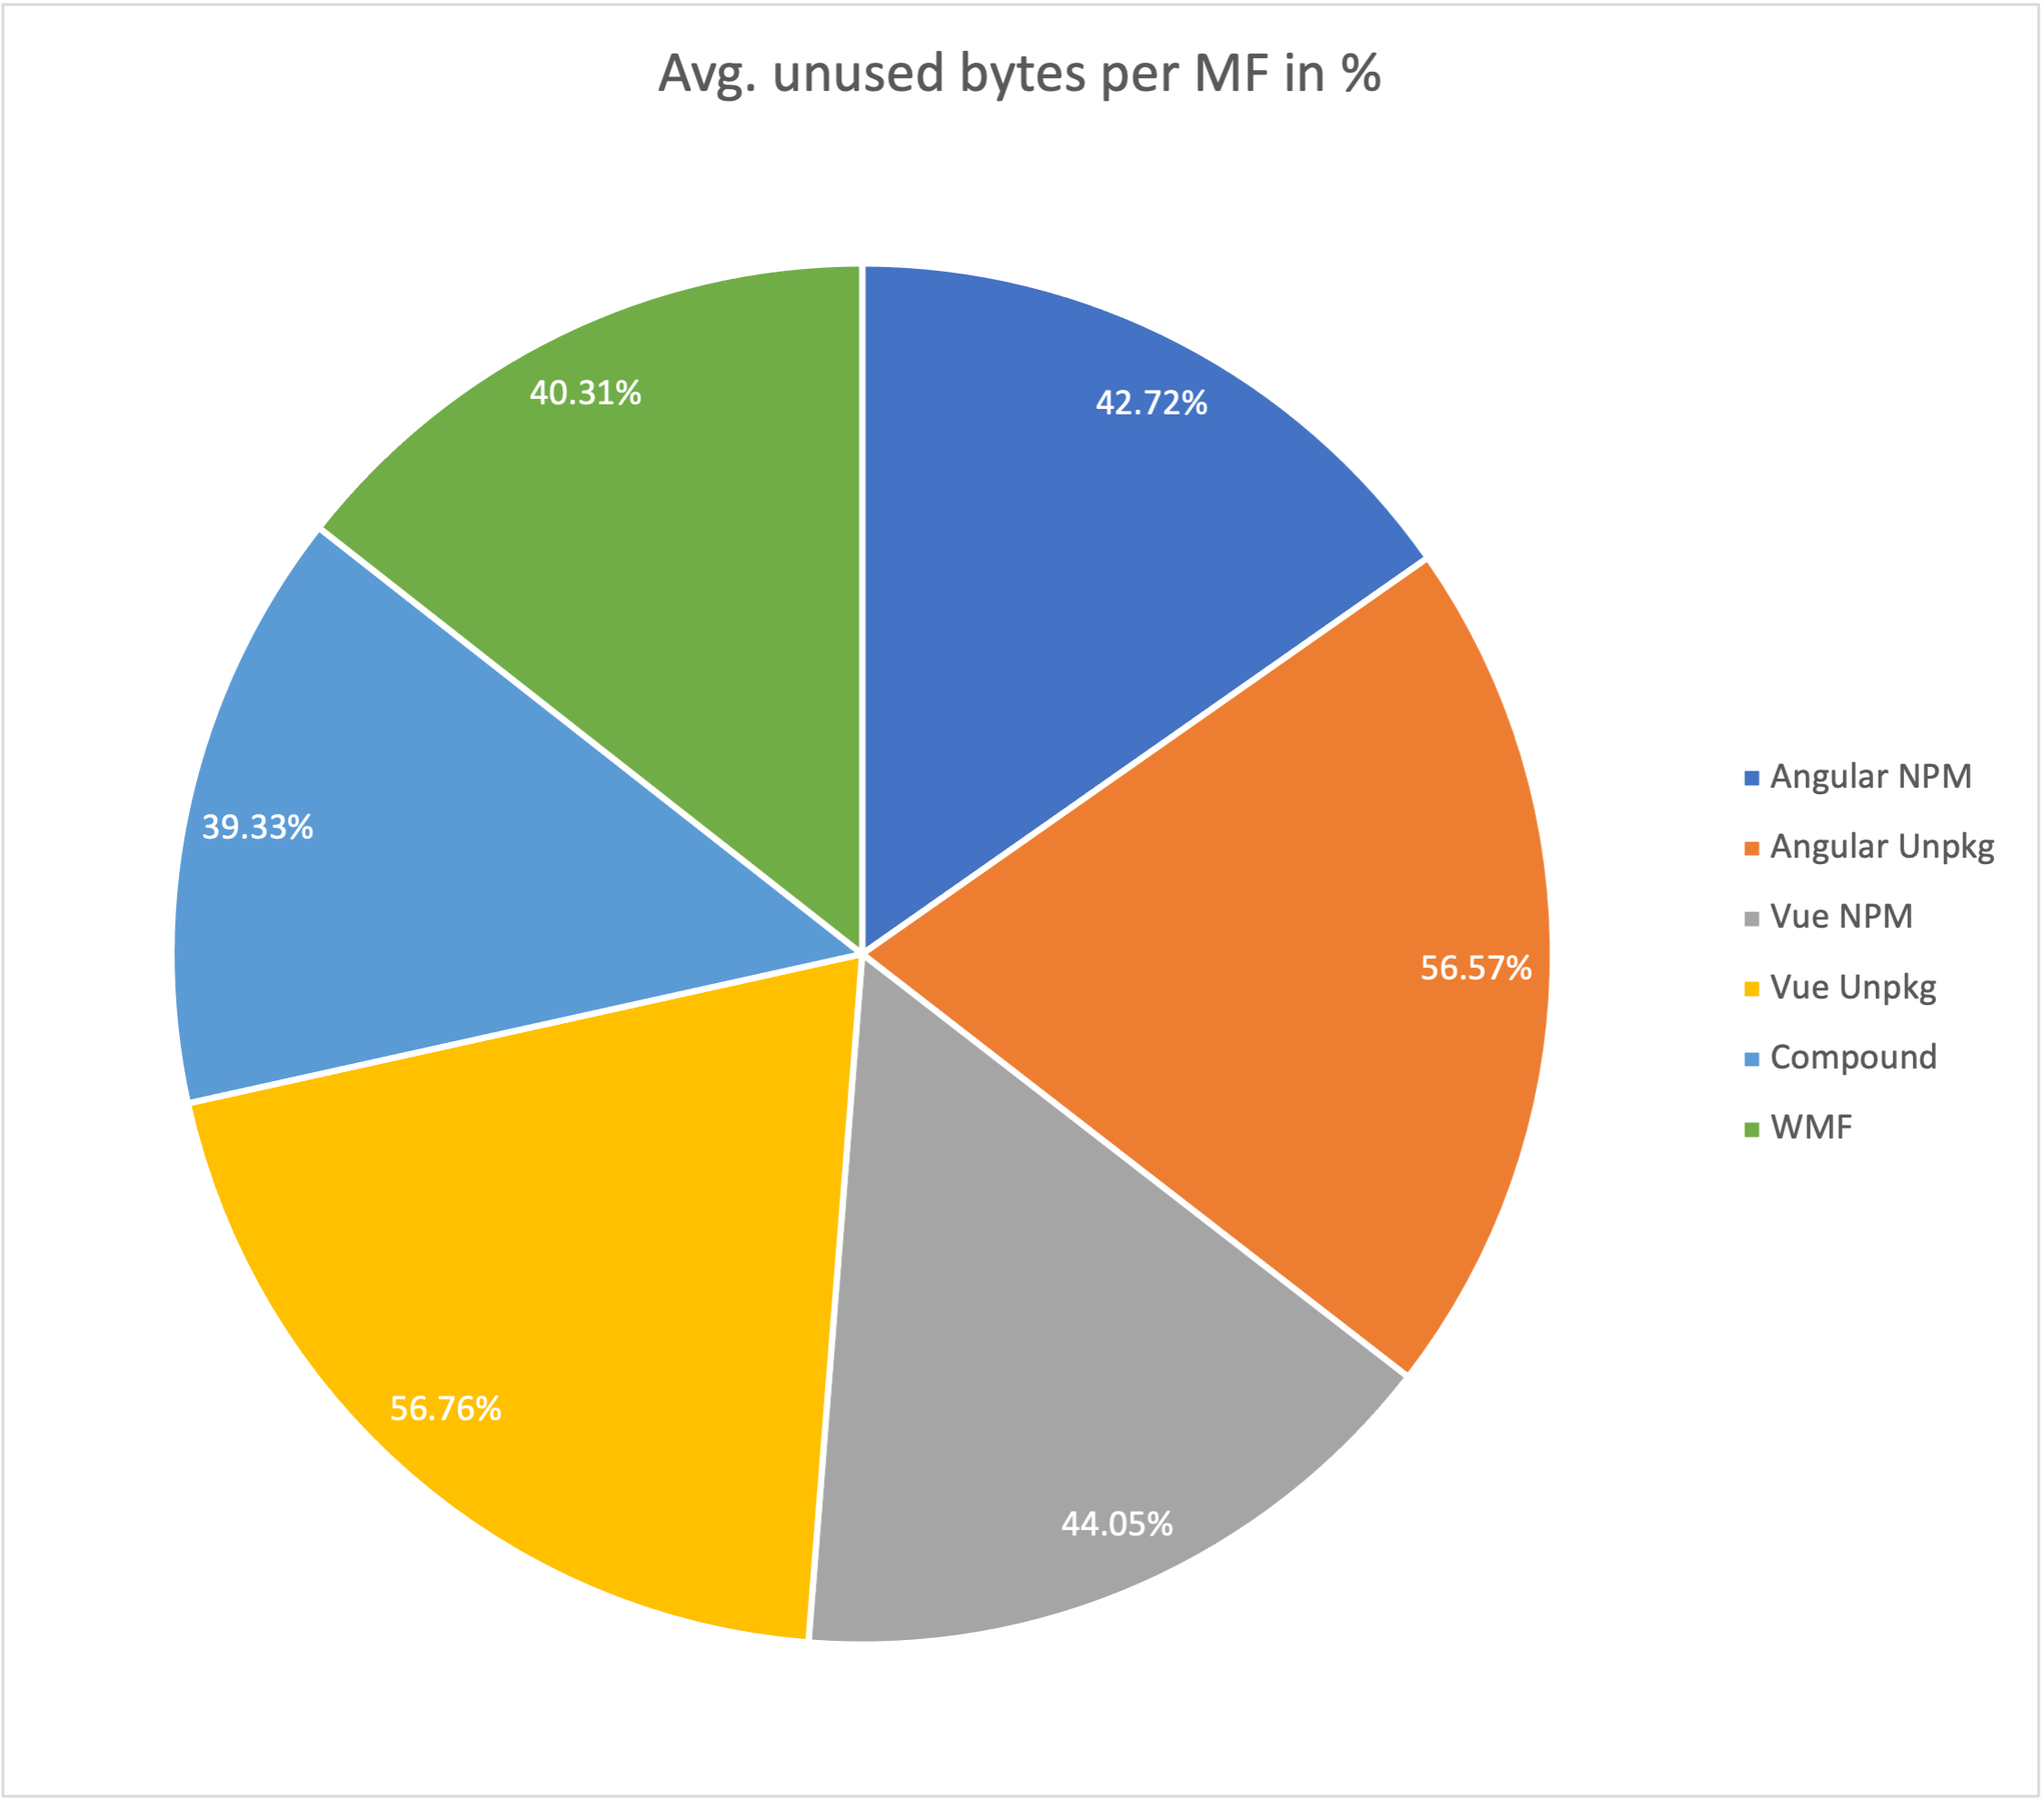
\includegraphics[width=1\textwidth]{Figures/avg_unsed_imported_2.png}
	\caption{Unused and imported bytes per landscape in \%}
	\label{fig:unsed_imported_2}
\end{figure}

The above shown data is highly application dependent. Still as these landscapes are considered to be generally representative, a display in efficiency can be drawn from the above shown charts.
The Unpkg CDN landscapes show a low unused bytes ratio. Since only the required resources were requested from the CDN, only a few unused bytes were detected by the Lighthouse tool. 
For the WMF landscape, it can be argued, that due to the bundling with Webpack, a lot of bytes were imported but only a few of them were not used. This can be explained through how the Module Federation works, since every configured shared resource is checked if it should be shared or not.

The following chapter will be concluding the displayed data. Detailed tables and information can be found in the appendixes \ref{appendix1}, \ref{appendix2} and \ref{appendix3}.

	% \glsresetall
\chapter{Presentation of the results} % Main chapter title
\label{Chapter7}

\lhead{Chapter 7. \emph{Presentation of the results}}

In this chapter it will be explained how and which data was collected using the prototype, and which metrics were defined for comparison.
Afterwards, the landscapes will be compared, using the defined metrics as KPIs. The conclusion based on the results will be given in chapter \ref{Chapter8}.

\section{Basis of the experiment} 

This section will contain information about the environment in which the experiment was executed, how the data was collected and which metrics were defined based on the gathered data.

\subsection{Testing hardware and environment}

It has to be mentioned, that certain aspects of the environment were not maintained by the tester and are therefore out of scope for influence or configuration. Nonetheless, they are mentioned here for the sake of reproducibility.
The following hardware and environment was used for testing:

\begin{enumerate}
	\item \textbf{Laptop:}
	\begin{itemize}[noitemsep]
		\item MacBook Pro (15-inch, 2017)
		\item \textbf{Processor:} 2.9 GHz Quad-Core Intel Core i7
		\item \textbf{Memory:} 16 GB 2133 MHz LPDDR3 
		\item \textbf{Graphics:} Radeon Pro 560 4 GB and Intel HD Graphics 630 1536 MB
		\item \textbf{macOS Monetary - Version:} 12.2.1 (21D62)
	\end{itemize} 
	
	\item \textbf{Browser, Network and Lighthouse:}
	\begin{itemize}[noitemsep]
		\item \textbf{Browser:} Google Chrome
		\item \textbf{Version:} 99.0.4844.51 (Official Build) (x86\_64)
		\item \textbf{Chrome DevTools version:} Chrome 99
		\item \textbf{Lighthouse version:} 100.0.0.0
		\item \textbf{JavaScript version:} V8 9.9.115.8
		\item \textbf{Network-Bandwidth:} 180-200 MB/s
	\end{itemize}
	
	\item \textbf{Runtime environment for prototypes:} surge.sh \footnote{surge.sh is a platform for static web publishing
		for frontend developers via the command line.}
	
	\item \textbf{CDN:} Unpkg.com \footnote{This part of the environment was explained in chapter \ref{Chapter6}}
\end{enumerate}

In addition to the specified hardware specs, version 1.18.1 of the \texttt{@luigi-project} was used. This dependency enables the Luigi framework and is therefore used in every implemented version of the prototype.

\subsection{Testing process}

Since multiple Nodes were implemented, a unified process was required to collect comparable data. The BPMN diagram \ref{fig:data_collection_process_har} contains the process steps in detail.

\begin{figure}[!h]
	\centering
	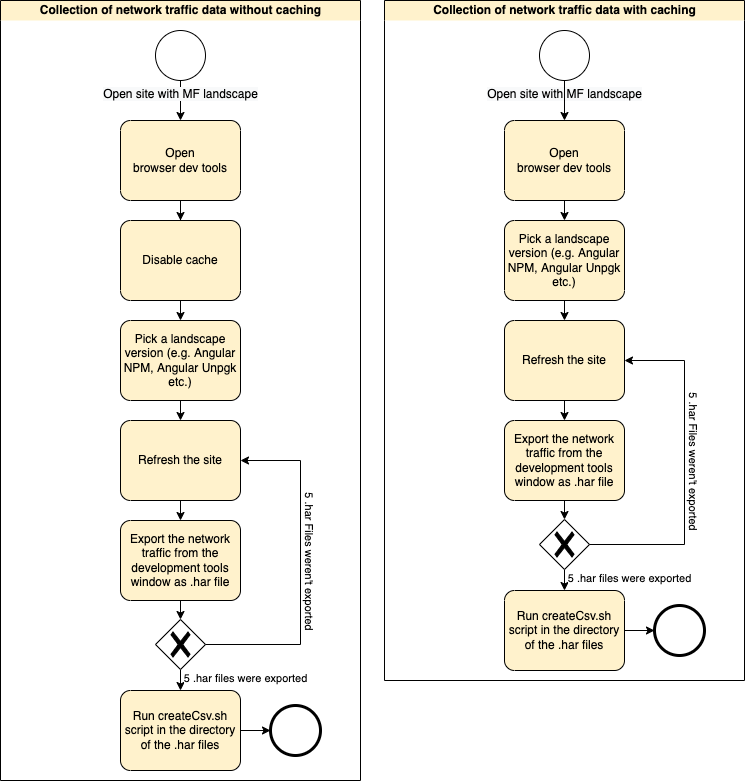
\includegraphics[width=0.7\textwidth]{Figures/Data_Collection_Process_har.drawio.png}
	\caption{Data collection process for .har files}
	\label{fig:data_collection_process_har}
\end{figure}

As it can be seen in \ref{fig:data_collection_process_har}, there were actually two processes executed to collect data. 
The first one had caching disabled, the second had it enabled. 
The intention behind the first process was to collect data for an average initial loading time for the picked site, therefore the resources must not be cached. 
The second process was used to gather information about caching behavior in general. 
Since each Node basically contains the same views, the browser should be able to pull already loaded resources from the cache, instead via the network. 
To showcase this behavior and prove the performance gain through caching, this data was gathered too.
Each process was executed 5 times, therefore 10 HTTP Archive (\texttt{.har}) files were generated per Node. 
These \texttt{.har} files were then transformed into \texttt{.csv} files using a self-developed script. 

Additionally to the \texttt{.har} files a website performance report was collected, using the Lighthouse tool embedded in the Google Chrome browser. Such a report provides information about how much of the imported bytes are actually used by a web application, distinguished by resource URL.

In summary, for testing:

\begin{itemize}[noitemsep]
	\item 12 Nodes were developed
	\item Each Node was loaded 10 times, 5 times with cache enabled and 5 times with cache disabled
	\item Each loading of a Node is represented by a HTTP Archive file
	\item All in all, the testing procedures were executed 120 times overall
	\item 120 \texttt{.har} files were generated
	\item These, were aggregated and transformed into 12 \texttt{.csv} files
	\item These, were copied into one Excel file, where the data was analyzed
	\item In addition, 12 Lighthouse reports where collected (one per Node) and added to the excel
\end{itemize}

The reason why this testing procedure was chosen, was due to the low variety in the parameters when a Node is loaded. First, it was tested if the parameters would vary when a Node is loaded up to 1000 times, but that was not the case. Due the constant resource sizes and stable network, not many fluctuations could be observed. Only when changes on technological level were made (e.g. usage of cache, network outage), fluctuations started to appear. But, other than that, it was observed that the results were stable. Therefore, it was decided that loading a Node 10 times would suffice for the experiment.

After the collection process, another self-developed script was used to aggregate all the gathered data into one single file. This file was later used to define and calculate the metrics, which are described next.

\subsection{Defined metrics}

The central file, containing all data, was split into separate sheets in which the metrics for each micro frontend were calculated. The parameters for calculation were:

\begin{description}
	\item[connection:] This is an ID with which each opened TCP connection is tagged by the browser. This value can be an indicator for the parallelity of the requests. Since the release of HTTP/2, several requests can be handled by a server via the same TCP connection, reducing the time costs for TCP handshakes. It has to be considered that the application requesting the sources can not implement this HTTP/2 feature. It has to be enabled on server-side and by the browser, which is already the case for most modern browsers \cite{http2}. As of today, surge.sh, the web server platform onto which the prototypes are deployed, does not support HTTP/2.
	
	\item[loadedFromCache:] This is a string value with three possible characteristics, \textit{not loaded from cache, disk} or \textit{memory}, whereas \textit{disk} and \textit{memory} are semantically the same. This value explains from where the resource was loaded. Either via the network from a remote server or from the local cache. It helps to indicate the caching behavior of bundled resources, in comparison with resources loaded from a unified URL (e.g. a CDN). 
	
	\item[startedDateTime:] This is a time stamp given to each request, marking its starting time in a DateTime format. This value can serve as an indicator for parallelity, since multiple TCP connections can be opened at the same time. 
	
	\item[requestUrl:] This is a string value, containing the request URL used by the browser to load the resource. This value mainly categorizes the calculation results, since neither \textit{connection} nor \textit{pageRef} are valid options to distinguish the loaded resources of a website. 
	
	\item[responseContentSize:] This number value is the byte size of the loaded resource.
	
	\item[timeInMs:] This value represents the RTT of the request in milliseconds. 
\end{description}

There were further parameters, available in the \texttt{.har} files, but those could not be used for the calculation. 
Based on the given metrics from the \texttt{.har} files, the following KPIs were calculated.

\begin{description}
	\item[Avg. Content Size:] Numerical value calculated by averaging the \textbf{responseContentSize} values of all the websites resources.
	
	\item[Avg. Time in MS Loaded values:] Numerical value, calculated by averaging the \textbf{timeInMs} values of all the websites resources.
	
	\item[Occurrences Connection Duplicates:] Numerical value to represent parallelity, by counting the number of duplicate/multiple occurring \textbf{connection} values.
	
	\item[Connection IDs:] List of all \textbf{connection} characteristics for the website.
	
	\item[Connection IDs occurrence:] Number of times the connection occurred during the loading of the website.
	
	\item[Parallel start time:] Numerical value, calculated by counting reoccurring \textbf{startedDateTime} values.
	
	\item[Avg. Response content size per Loading Type:] Numerical value, calculated by averaging the \textbf{responseContentSize}, differentiated by the characteristics of the \textbf{loadedFromCache} property.
	
	\item[URLs loaded:] List of all unique \textbf{requestUrl} values.
	
	\item[Avg. Response Time per URL loaded in MS:] Numerical value, representing the average loading time of each loaded resource URL of the website.
	
	\item[Avg. Response Size per URL loaded:] Numerical value, representing the average loading byte size of each resource URL.
	
	\item[Avg. Response Size per URL loaded via networkbel:] - Numerical value, calculated by averaging the \textbf{responseContentSize} differentiated by the \textbf{requestUrl} for all resources with the \textbf{loadedFromCache} value of \textit{not loaded from cache}. For the test scenarios with cache disabled, this value equals the \textbf{Avg. Response Size per URL loaded} KPI.
	
	\item[Avg. Response Size per URL loaded from Disk:] Numerical value, calculated by averaging the \textbf{responseContentSize} differentiated by the \textbf{requestUrl}, for all resources with the \textbf{loadedFromCache} value of \textit{disk}.
	
	\item[Avg. Response Size per URL loaded from Memory:] Numerical value, calculated by averaging the \textbf{responseContentSize} differentiated by the \textbf{requestUrl}, for all resources with the \textbf{loadedFromCache} value of \textit{memory}.
\end{description}

The main indicators for whether a technology successfully reduces redundant libraries in a micro frontend landscapes were the \textbf{Avg. Time in MS Loaded values} and \textbf{Avg. Content Size}. 
Therefore, the goal was to optimize these two KPIs. If, by using a technology, these two values decreased, it was considered to be a first success. 
But, for the general evaluation, further aspects were put into consideration. 
KPIs for those aspects, such as e.g. the complexity of the implemented technology, were hard to measure.  
A metric like this must not be ignored for the context of this transcript, since the benefit of a technology highly depends on it.
Thus, the subjective estimation and impression of the used technologies by the author is part of the conclusion in chapter \ref{Chapter8}.

Statistical values, like the median ,were calculated, but not included in the conclusion, since the meaningfulness of those values was not applicable for the goal. The package size does affect loading time of a resources, that is a matter of fact. But since the packages are application-specific, no general statement can be drawn from the median of this parameters. The goal was to showcase that through the usage of one of the three technologies, the loading times and loaded bytes are reduced in general, not to show what package is not loaded or loaded faster.

In the following sections, the results of the introduced metrics for each landscape are showcased. 
The tables shown, are separated whether or not, the data was collected with caching enabled or disabled. 
In addition, to the shown metrics, the graphs and Excel tables for the landscapes are referred to in the archive.
A table of contents of the archive is available in appendix \ref{appendix1}.

\section{CDN/NPM KPI results}

This section will introduce the KPI results of the CDN/NPM prototype. It is split into two subsections for a better comparison of the two technologies.

\subsection{Implementation with NPM}

Table \ref{tab:cdn_result_table} contains the results for the implemented Nodes with a regular bundler and a package manager, namely NPM. 
Certain metrics are not added to the table for readability, but a graphical representation can be found in in the archive.

\scriptsize
\setlength{\mycolwidth}{\dimexpr \textwidth/5 - 2\tabcolsep}

\begin{longtable}[c]{*{3}{p{\mycolwidth}}}
	
	\caption{Table of numerical KPI results for the NPM Nodes with caching disabled}
	\label{tab:cdn_result_table} \\
	
	\toprule
	\multicolumn{1}{l}{\makecell[c]{\textbf{Metric}}}   
	& \multicolumn{1}{l}{\makecell[c]{\textbf{Angular NPM}}}                              
	& \multicolumn{1}{l}{\makecell[c]{\textbf{Vue NPM}}} \\ 
	\midrule
	\endfirsthead
	
	\multicolumn{3}{l}{\footnotesize\itshape\tablename~\thetable:
		continued from previous page} \\
	\toprule   
	\multicolumn{1}{l}{\makecell[c]{\textbf{Metric}}}   
	& \multicolumn{1}{l}{\makecell[c]{\textbf{Angular NPM}}}                              
	& \multicolumn{1}{l}{\makecell[c]{\textbf{Vue NPM}}} \\*
	\midrule
	\endhead
	%		
	\multicolumn{1}{l|}{URLs loaded count}                                         															
	& \multicolumn{1}{l|}{\makecell[c]{14}} 	
	& \multicolumn{1}{l}{\makecell[c]{13}}   \\ \midrule
	
	\multicolumn{1}{l|}{\makecell[l]{Avg. Response content size\\per Loading Type}}   
	& \multicolumn{1}{l|}{\makecell[c]{\textit{not loaded from cache} - 129529.13, \\ \textit{memory} - 0, \\ \textit{disk} - 0}} 											
	& \multicolumn{1}{l}{\makecell[c]{\textit{not loaded from cache} - 156131.63, \\ \textit{memory} - 0, \\ \textit{disk} - 0}}   \\ \midrule
	
	\multicolumn{1}{l|}{Parallel start time}                                 													
	& \multicolumn{1}{l|}{\makecell[c]{33}} 				
	& \multicolumn{1}{l}{\makecell[c]{45}}   \\ \midrule
	
	\multicolumn{1}{l|}{Connection IDs occurence}                            											
	& \multicolumn{1}{l|}{\makecell[c]{\textit{none established} - 10,\\ \textit{207393} - 10}} 												   
	& \multicolumn{1}{l}{\makecell[c]{\textit{241394} - 10}}   \\ \midrule
	
	\multicolumn{1}{l|}{Connection IDs count}                                      																
	& \multicolumn{1}{l|}{\makecell[c]{62}} 															     
	& \multicolumn{1}{l}{\makecell[c]{71}}   \\ \midrule
		
	\multicolumn{1}{l|}{\makecell[l]{Connection Duplicates}}                        
	& \multicolumn{1}{l|}{\makecell[c]{20}} 						   
	& \multicolumn{1}{l}{\makecell[c]{10}}   \\ \midrule
	
	\multicolumn{1}{l|}{\makecell[l]{Loaded values \& occurrences}}                        
	& \multicolumn{1}{c|}{\makecell[c]{\textit{not loaded from cache} - 80,\\ \textit{memory} - 0, \\ \textit{disk} - 0}} 						   
	& \multicolumn{1}{l}{\makecell[c]{\textit{not loaded from cache} - 80, \\ \textit{memory} - 0, \\ \textit{disk} - 0}}   \\ \midrule
	
	\multicolumn{1}{l|}{\makecell[l]{Avg. Time in MS}}                        
	& \multicolumn{1}{l|}{\makecell[c]{162.22}} 						   
	& \multicolumn{1}{l}{\makecell[c]{5323.54}}   \\ \midrule
	
	\multicolumn{1}{l|}{\makecell[l]{Avg. Content Size}}                                         
	& \multicolumn{1}{l|}{\makecell[c]{129529.13}}  				  
	&   \multicolumn{1}{l}{\makecell[c]{156131.63}} \\ \bottomrule
\end{longtable}

\normalsize
The results shown in table \ref{tab:cdn_result_table} were collected without caching enabled. 
This explains for instance, why no resources were loaded from cache and therefore, why the values for the \textit{memory} or \textit{disk} characteristics are missing.
The main takeaway from these results is an average initial loading time for the Nodes, which differs depending on the framework. 
It can also be seen that even though fewer resources are loaded via URLs by the Vue.js Nodes, they have a longer loading time compared to the Angular ones.

\scriptsize
\setlength{\mycolwidth}{\dimexpr \textwidth/5 - 2\tabcolsep}

\begin{longtable}[c]{*{3}{p{\mycolwidth}}}
	
	\caption{Table of numerical KPI results for the NPM Nodes with caching enabled}
	\label{tab:cdn_result_table_caching} \\
	
	\toprule
	\multicolumn{1}{l}{\makecell[c]{\textbf{Metric}}}   
	& \multicolumn{1}{l}{\makecell[c]{\textbf{Angular NPM}}}                              
	& \multicolumn{1}{l}{\makecell[c]{\textbf{Vue NPM}}} \\ 
	\midrule
	\endfirsthead
	
	\multicolumn{3}{l}{\footnotesize\itshape\tablename~\thetable:
		continued from previous page} \\
	\toprule   
	\multicolumn{1}{l}{\makecell[c]{\textbf{Metric}}}   
	& \multicolumn{1}{l}{\makecell[c]{\textbf{Angular NPM}}}                              
	& \multicolumn{1}{l}{\makecell[c]{\textbf{Vue NPM}}} \\*
	\midrule
	\endhead
	%		
	\multicolumn{1}{l|}{URLs loaded count}                                         															
	& \multicolumn{1}{l|}{\makecell[c]{14}} 	
	& \multicolumn{1}{l}{\makecell[c]{13}}   \\ \midrule
	
	\multicolumn{1}{l|}{\makecell[l]{Avg. Response content size\\per Loading Type}}   
	& \multicolumn{1}{l|}{\makecell[c]{\textit{not loaded from cache} - 166856, \\ \textit{memory} - 17548.5, \\ \textit{disk} - 17548.5}} 											
	& \multicolumn{1}{l}{\makecell[c]{\textit{not loaded from cache} - 145646.67,\\ \textit{memory} - 0, \\ \textit{disk} - 187586.5}}   \\ \midrule
	
	\multicolumn{1}{l|}{Parallel start time}                                 													
	& \multicolumn{1}{l|}{\makecell[c]{32}} 				
	& \multicolumn{1}{l}{\makecell[c]{39}}   \\ \midrule
	
	\multicolumn{1}{l|}{Connection IDs occurence}                            											
	& \multicolumn{1}{l|}{\makecell[c]{\textit{none established} - 20}} 												   
	& \multicolumn{1}{l}{\makecell[c]{\textit{none established} - 20}}   \\ \midrule
	
	\multicolumn{1}{l|}{Connection IDs count}                                      																
	& \multicolumn{1}{l|}{\makecell[c]{61}} 															     
	& \multicolumn{1}{l}{\makecell[c]{61}}   \\ \midrule
	
	\multicolumn{1}{l|}{\makecell[l]{Connection Duplicates}}                        
	& \multicolumn{1}{l|}{\makecell[c]{20}} 						   
	& \multicolumn{1}{l}{\makecell[c]{20}}   \\ \midrule
	
	\multicolumn{1}{l|}{\makecell[l]{Loaded values \& occurrences}}                        
	& \multicolumn{1}{c|}{\makecell[c]{\textit{not loaded from cache} - 60, \\ \textit{memory} - 6, \\ \textit{disk} - 14}} 						   
	& \multicolumn{1}{l}{\makecell[c]{\textit{not loaded from cache} - 60, \\ \textit{memory} - 0, \\ \textit{disk} - 20}}   \\ \midrule
	
	\multicolumn{1}{l|}{\makecell[l]{Avg. Time in MS}}                        
	& \multicolumn{1}{l|}{\makecell[c]{150.90}} 						   
	& \multicolumn{1}{l}{\makecell[c]{1890.6}}   \\ \midrule
	
	\multicolumn{1}{l|}{\makecell[l]{Avg. Content Size}}                                         
	& \multicolumn{1}{l|}{\makecell[c]{129529.13}}  				  
	&   \multicolumn{1}{l}{\makecell[c]{156131.63}} \\ \bottomrule
	
\end{longtable}

\normalsize
The results of table \ref{tab:cdn_result_table_caching} show the effect caching has on the performance of a site. 
The average loading time of the site decreases, as do the opened TCP connections.

Both environments were implemented using a regular bundler, it can therefore not be ensured that redundant libraries were not loaded.

\subsection{Implementation with Unpkg.com}

Table \ref{tab:cdn_result_table_unpkg} contains the results for the implemented Nodes with a use of a public CDN, namely Unpkg.com. 
Certain metrics are not added to the table for readability, but a graphical representation can be found in archive. 

\scriptsize
\setlength{\mycolwidth}{\dimexpr \textwidth/5 - 2\tabcolsep}

\begin{longtable}[c]{*{3}{p{\mycolwidth}}}
	
	\caption{Table of numerical KPI results for the Nodes using the Unpkg.com CDN with caching disabled}
	\label{tab:cdn_result_table_unpkg} \\
	
	\toprule
	\multicolumn{1}{l}{\makecell[c]{\textbf{Metric}}}   
	& \multicolumn{1}{l}{\makecell[c]{\textbf{Angular Unpkg}}}                              
	& \multicolumn{1}{l}{\makecell[c]{\textbf{Vue Unpkg}}} \\ 
	\midrule
	\endfirsthead
	
	\multicolumn{3}{l}{\footnotesize\itshape\tablename~\thetable:
		continued from previous page} \\
	\toprule                        
	\multicolumn{1}{l}{\makecell[c]{\textbf{Metric}}}   
	& \multicolumn{1}{l}{\makecell[c]{\textbf{Angular Unpkg}}}                              
	& \multicolumn{1}{l}{\makecell[c]{\textbf{Vue Unpkg}}} \\*
	\midrule
	\endhead
	%		
	\multicolumn{1}{l|}{URLs loaded count}                                         															
	& \multicolumn{1}{l|}{\makecell[c]{171}} 	
	& \multicolumn{1}{l}{\makecell[c]{165}}   \\ \midrule
	
	\multicolumn{1}{l|}{\makecell[l]{Avg. Response content size\\per Loading Type}}   
	& \multicolumn{1}{l|}{\makecell[c]{\textit{not loaded from cache} - 9768.62, \\ \textit{memory} - 0, \\ \textit{disk} - 0}} 											
	& \multicolumn{1}{l}{\makecell[c]{\textit{not loaded from cache} - 8205.19, \\ \textit{memory} - 0, \\ \textit{disk} - 0}}   \\ \midrule
	
	\multicolumn{1}{l|}{Parallel start time}                                 													
	& \multicolumn{1}{l|}{\makecell[c]{871}} 				
	& \multicolumn{1}{l}{\makecell[c]{989}}   \\ \midrule
	
	\multicolumn{1}{l|}{Connection IDs occurence}                            											
	& \multicolumn{1}{l|}{\makecell[c]{\textit{223736} - 20,\\ \textit{223722} - 1574,\\ \textit{none established} - 10}} 												   
	& \multicolumn{1}{l}{\makecell[c]{\textit{241394} - 20,\\ \textit{249654} - 1560}}   \\ \midrule
	
	\multicolumn{1}{l|}{Connection IDs count}                                      																
	& \multicolumn{1}{l|}{\makecell[c]{53}} 															     
	& \multicolumn{1}{l}{\makecell[c]{42}}   \\ \midrule
	
	\multicolumn{1}{l|}{\makecell[l]{Connection Duplicates}}                        
	& \multicolumn{1}{l|}{\makecell[c]{1604}} 						   
	& \multicolumn{1}{l}{\makecell[c]{1580}}   \\ \midrule
	
	\multicolumn{1}{l|}{\makecell[l]{Loaded values \&\\ occurrences}}                        
	& \multicolumn{1}{c|}{\makecell[c]{\textit{not loaded from cache} - 1654, \\ \textit{memory} - 0, \\ \textit{disk} - 0}} 						   
	& \multicolumn{1}{l}{\makecell[c]{\textit{not loaded from cache} - 1620, \\ \textit{memory} - 0, \\ \textit{disk} - 0}}   \\ \midrule
	
	\multicolumn{1}{l|}{\makecell[l]{Avg. Time in MS}}                        
	& \multicolumn{1}{l|}{\makecell[c]{97.23}} 						   
	& \multicolumn{1}{l}{\makecell[c]{194.01}}   \\ \midrule
	
	\multicolumn{1}{l|}{\makecell[l]{Avg. Content Size}}                                         
	& \multicolumn{1}{l|}{\makecell[c]{9768.62}}  				  
	&   \multicolumn{1}{l}{\makecell[c]{8205.19}} \\ \bottomrule
	
\end{longtable}

\normalsize
The data shown in table \ref{tab:cdn_result_table_unpkg} has again been collected without caching enabled.
An approximate estimation for the initial loading times can be drawn from this. 
It becomes apparent that the Vue.js environment takes longer to load for less content. 
A similar behavior was observed in the NPM implementations.
Nonetheless, it is an improvement in performance compared to the NPM counterparts for both Nodes. 
The trade-off of this technology is that single component resources, like a button or a table, had to be imported via script tags one by one, thus the increase in loaded URLs.

\scriptsize
\setlength{\mycolwidth}{\dimexpr \textwidth/5 - 2\tabcolsep}

\begin{longtable}[c]{*{3}{p{\mycolwidth}}}
 	
 	\caption{Table of numerical KPI results for the Nodes using the Unpkg.com CDN with caching enabled}
 	\label{tab:cdn_result_table_unpkg_cache} \\
 	
 	\toprule
	\multicolumn{1}{l}{\makecell[c]{\textbf{Metric}}}   
	& \multicolumn{1}{l}{\makecell[c]{\textbf{Angular Unpkg}}}                              
	& \multicolumn{1}{l}{\makecell[c]{\textbf{Vue Unpkg}}} \\ 
 	\midrule
 	\endfirsthead
 	
 	\multicolumn{3}{l}{\footnotesize\itshape\tablename~\thetable:
 		continued from previous page} \\
 	\toprule   
	\multicolumn{1}{l}{\makecell[c]{\textbf{Metric}}}   
	& \multicolumn{1}{l}{\makecell[c]{\textbf{Angular Unpkg}}}                              
	& \multicolumn{1}{l}{\makecell[c]{\textbf{Vue Unpkg}}} \\*
 	\midrule
 	\endhead
 	%		
 	\multicolumn{1}{l|}{URLs loaded count}                                         															
 	& \multicolumn{1}{l|}{\makecell[c]{171}} 	
 	& \multicolumn{1}{l}{\makecell[c]{165}}   \\ \midrule
 	
 	\multicolumn{1}{l|}{\makecell[l]{Avg. Response content size\\per Loading Type}}   
 	& \multicolumn{1}{l|}{\makecell[c]{\textit{not loaded from cache} - 63972.08, \\ \textit{memory} - 208838, \\ \textit{disk} - 7166.1}} 											
 	& \multicolumn{1}{l}{\makecell[c]{\textit{not loaded from cache} - 28143.2, \\ \textit{memory} - 0, \\ \textit{disk} - 7570.22}}   \\ \midrule
 	
 	\multicolumn{1}{l|}{Parallel start time}                                 													
 	& \multicolumn{1}{l|}{\makecell[c]{1111}} 				
 	& \multicolumn{1}{l}{\makecell[c]{1069}}   \\ \midrule
 	
 	\multicolumn{1}{l|}{Connection IDs occurence}                            											
 	& \multicolumn{1}{l|}{\makecell[c]{\textit{none established} - 1590,\\ \textit{223722} - 15}} 												   
 	& \multicolumn{1}{l}{\makecell[c]{\textit{none established} - 1570,\\ \textit{249654} - 10}}   \\ \midrule
 	
 	\multicolumn{1}{l|}{Connection IDs count}                                      																
 	& \multicolumn{1}{l|}{\makecell[c]{52}} 															     
 	& \multicolumn{1}{l}{\makecell[c]{42}}   \\ \midrule
 	
 	\multicolumn{1}{l|}{\makecell[l]{Connection Duplicates}}                        
 	& \multicolumn{1}{l|}{\makecell[c]{1605}} 						   
 	& \multicolumn{1}{l}{\makecell[c]{1580}}   \\ \midrule
 	
 	\multicolumn{1}{l|}{\makecell[l]{Loaded values \& occurrences}}                        
 	& \multicolumn{1}{c|}{\makecell[c]{\textit{not loaded from cache} - 65, \\ \textit{memory} - 3, \\ \textit{disk} - 1587}} 						   
 	& \multicolumn{1}{l}{\makecell[c]{\textit{not loaded from cache} - 50, \\ \textit{memory} - 0, \\ \textit{disk} - 1570}}   \\ \midrule
 	
 	\multicolumn{1}{l|}{\makecell[l]{Avg. Time in MS}}                        
 	& \multicolumn{1}{l|}{\makecell[c]{58.73}} 						   
 	& \multicolumn{1}{l}{\makecell[c]{87.1}}   \\ \midrule
 	
 	\multicolumn{1}{l|}{\makecell[l]{Avg. Content Size}}                                         
 	& \multicolumn{1}{l|}{\makecell[c]{9762.72}}  				  
 	&   \multicolumn{1}{l}{\makecell[c]{8205.19}} \\ \bottomrule
 	
\end{longtable}

\normalsize
A similar development can be observed in table \ref{tab:cdn_result_table_unpkg_cache}. Firstly, with caching enabled, the average loading times decrease. Secondly, the number of loaded resources from cache increases significantly, and lastly, the Angular environments show shorter average loading times, despite more resources being requested via URL by them.

\section{Web Components and WMF landscapes}

As the described in chapter \ref{Chapter6}, these environments exist in different versions. They were designed that way to showcase how the used technologies handle multi-version landscapes and how they affect the performance.
Table \ref{tab:wmf_compound} shows the KPIs of those environments.
 
\scriptsize
\setlength{\mycolwidth}{\dimexpr \textwidth/5 - 2\tabcolsep}

\begin{longtable}[c]{*{3}{p{\mycolwidth}}}
	
	\caption{Table of numerical KPI results, for the Nodes implemented with Web Components and WMF as compounds, with caching disabled}
	\label{tab:wmf_compound} \\
	
	\toprule
	\multicolumn{1}{l}{\makecell[c]{\textbf{Metric}}}   
	& \multicolumn{1}{l}{\makecell[c]{\textbf{Web Components}}}                              
	& \multicolumn{1}{l}{\makecell[c]{\textbf{WMF}}} \\ 
	\midrule
	\endfirsthead
	
	\multicolumn{3}{l}{\footnotesize\itshape\tablename~\thetable: continued from previous page} \\
	\toprule                        
	\multicolumn{1}{l}{\makecell[c]{\textbf{Metric}}}   
	& \multicolumn{1}{l}{\makecell[c]{\textbf{Web Components}}}                              
	& \multicolumn{1}{l}{\makecell[c]{\textbf{WMF}}} \\*
	\midrule
	\endhead
	%		
	\multicolumn{1}{l|}{URLs loaded count}                                         															
	& \multicolumn{1}{l|}{\makecell[c]{27}} 	       
	& \multicolumn{1}{l}{\makecell[c]{118}}   \\ \midrule
	
	\multicolumn{1}{l|}{\makecell[l]{Avg. Response content size\\per Loading Type}}   
	& \multicolumn{1}{l|}{\makecell[c]{\textit{not loaded from cache} - 213266.74, \\ \textit{memory} - 0,\\ \textit{disk} - 0}} 			         
	& \multicolumn{1}{l}{\makecell[c]{\textit{not loaded from cache} - 507168.76, \\ \textit{memory} - 0, \\ \textit{disk} - 0}}   \\ \midrule
	
	\multicolumn{1}{l|}{Parallel start time}                                 													
	& \multicolumn{1}{l|}{\makecell[c]{29}} 				                  
	& \multicolumn{1}{l}{\makecell[c]{109}}   \\ \midrule
	
	\multicolumn{1}{l|}{Connection IDs occurence}                            											
	& \multicolumn{1}{l|}{\makecell[c]{\textit{78725} - 15,\\ \textit{78890} - 15}} 		              
	& \multicolumn{1}{l}{\makecell[c]{\textit{728247} - 3,\\ \textit{none established} - 14}}   \\ \midrule
	
	\multicolumn{1}{l|}{Connection IDs count}                                      																
	& \multicolumn{1}{l|}{\makecell[c]{546}} 		         											     
	& \multicolumn{1}{l}{\makecell[c]{42}}   \\ \midrule
	
	\multicolumn{1}{l|}{\makecell[l]{Connection Duplicates}}                        
	& \multicolumn{1}{l|}{\makecell[c]{30}} 					
	& \multicolumn{1}{l}{\makecell[c]{20}}   \\ \midrule
	
	\multicolumn{1}{l|}{\makecell[l]{Loaded values \& occurrences}}                          
	& \multicolumn{1}{c|}{\makecell[c]{\textit{not loaded from cache} - 135, \\ \textit{memory} - 30, \\ \textit{disk} - 0}} 						   
	& \multicolumn{1}{l}{\makecell[c]{\textit{not loaded from cache} - 563, \\ \textit{memory} - 0, \\ \textit{disk} - 0}}   \\ \midrule
	
	\multicolumn{1}{l|}{\makecell[l]{Avg. Time in MS}}                        
	& \multicolumn{1}{l|}{\makecell[c]{2454.95}} 	                			   
	& \multicolumn{1}{l}{\makecell[c]{552.7}}   \\ \midrule
	
	\multicolumn{1}{l|}{\makecell[l]{Avg. Content Size}}                                         
	& \multicolumn{1}{l|}{\makecell[c]{213266.74}}  		          
	&   \multicolumn{1}{l}{\makecell[c]{507168.76}} \\ \bottomrule
	
\end{longtable}

\normalsize
As the data in table \ref{tab:wmf_compound} shows, the initial loading time for the Web Component environments is significantly lower compared to the WMF counterpart. Also the number of loaded resources differs. This is due to the fact that WMF has to be used in combination with the Webpack 5 bundler. Therefore, certain resources might be loaded several times, if not configured as shared dependencies in the Module Federation. 
Table \ref{tab:wmf_compound_cache} showcases the same landscapes, but with caching enabled.

\scriptsize
\setlength{\mycolwidth}{\dimexpr \textwidth/5 - 2\tabcolsep}

\begin{longtable}[c]{*{3}{p{\mycolwidth}}}
	
	\caption{Table of numerical KPI results, for the Nodes implemented with Web Components and WMF as compounds, with caching enabled}
	\label{tab:wmf_compound_cache} \\
	
	\toprule
	\multicolumn{1}{l}{\makecell[c]{\textbf{Metric}}}   
	& \multicolumn{1}{l}{\makecell[c]{\textbf{Web Components}}}                              
	& \multicolumn{1}{l}{\makecell[c]{\textbf{WMF}}} \\ 
	\midrule
	\endfirsthead
	
	\multicolumn{3}{l}{\footnotesize\itshape\tablename~\thetable: continued from previous page} \\
	\toprule                        
	\multicolumn{1}{l}{\makecell[c]{\textbf{Metric}}}   
	& \multicolumn{1}{l}{\makecell[c]{\textbf{Web Components}}}                              
	& \multicolumn{1}{l}{\makecell[c]{\textbf{WMF}}} \\*
	\midrule
	\endhead
	%		
	\multicolumn{1}{l|}{URLs loaded count}                                         															
	& \multicolumn{1}{l|}{\makecell[c]{27}} 	       
	& \multicolumn{1}{l}{\makecell[c]{109}}   \\ \midrule
	
	\multicolumn{1}{l|}{\makecell[l]{Avg. Response content size\\per Loading Type}}   
	& \multicolumn{1}{l|}{\makecell[c]{\textit{not loaded from cache} - 215385.36, \\ \textit{memory} - 167973, \\ \textit{disk} - 588082}} 			         
	& \multicolumn{1}{l}{\makecell[c]{\textit{not loaded from cache} - 525243.08, \\ \textit{memory} - 0, \\ \textit{disk} - 1959}}   \\ \midrule
	
	\multicolumn{1}{l|}{Parallel start time}                                 													
	& \multicolumn{1}{l|}{\makecell[c]{35}} 				                  
	& \multicolumn{1}{l}{\makecell[c]{105}}   \\ \midrule
	
	\multicolumn{1}{l|}{Connection IDs occurence}                            											
	& \multicolumn{1}{l|}{\makecell[c]{\textit{none established} - 4,\\ \textit{78890} - 15,\\ \textit{78725} - 11}} 		              
	& \multicolumn{1}{l}{\makecell[c]{\textit{none established} - 15}}   \\ \midrule
	
	\multicolumn{1}{l|}{Connection IDs count}                                      																
	& \multicolumn{1}{l|}{\makecell[c]{104}} 		         											     
	& \multicolumn{1}{l}{\makecell[c]{537}}   \\ \midrule
	
	\multicolumn{1}{l|}{\makecell[l]{Connection Duplicates}}                        
	& \multicolumn{1}{l|}{\makecell[c]{30}} 					
	& \multicolumn{1}{l}{\makecell[c]{15}}   \\ \midrule
	
	\multicolumn{1}{l|}{\makecell[l]{Loaded values \& occurrences}}                          
	& \multicolumn{1}{c|}{\makecell[c]{\textit{not loaded from cache} - 107, \\ \textit{memory} - 20, \\ \textit{disk} - 4}} 						   
	& \multicolumn{1}{l}{\makecell[c]{\textit{not loaded from cache} - 536, \\ \textit{memory} - 0, \\ \textit{disk} - 15}}   \\ \midrule
	
	\multicolumn{1}{l|}{\makecell[l]{Avg. Time in MS}}                        
	& \multicolumn{1}{l|}{\makecell[c]{897.62}} 	                			   
	& \multicolumn{1}{l}{\makecell[c]{356.53}}   \\ \midrule
	
	\multicolumn{1}{l|}{\makecell[l]{Avg. Content Size}}                                         
	& \multicolumn{1}{l|}{\makecell[c]{219526.89}}  		          
	&   \multicolumn{1}{l}{\makecell[c]{510997.6}} \\ \bottomrule
	
\end{longtable}

\normalsize
The general results appear to be similar for both cases of caching en- or disabled. The only KPI in favor of Web Components is the average content size loaded. 
Additionally, compared to the Web Component Nodes the WMF Nodes cache little to none resources. 

To add further parameters into the decision making process for the final conclusion, the Lighthouse tool was used. 
Through it, more information about the prototypes was gathered. 
The next section will showcase and explain how the analysis was done.

\section{Lighthouse analysis}

For the Lighthouse analysis, it was put into consideration that the reports are application-specific. 
But since the prototypes are considered to be representative, it is assumed that similar results can be expected in general from other micro frontend landscapes. 
Exception are not excluded from this assumption.

The given data was gathered based on the previously introduced prototypes and their Nodes. 
It contains the analysis of the imported resources and how much of the corresponding imports were not used by the application, measured in bytes. 
First, a tabular view is provided, followed by the corresponding graph.

\newpage

\scriptsize 
\setlength{\mycolwidthtwo}{\dimexpr \textwidth/5 - 2\tabcolsep}%

\begin{longtable}[c]{*{4}{p{\mycolwidthtwo}}}
	
	\caption{Table of the average imported and unused bytes of the prototypes, collected via the Lighthouse tool}
	\label{tab:lighthouse_used_report} \\
	
	\toprule
	\textbf{Landscape}                        
	& \multicolumn{1}{l}{\makecell[c]{\textbf{Avg. imported bytes}}}   
	& \multicolumn{1}{l}{\makecell[c]{\textbf{Avg. unused bytes}}}                              
	& \multicolumn{1}{l}{\makecell[c]{\textbf{Avg. unused bytes in \%}}} \\                                    
	\midrule
	\endfirsthead
	
	\multicolumn{4}{l}{\footnotesize\itshape\tablename~\thetable: continued from previous page} \\
	\toprule        
	\textbf{Landscape}                        
	& \multicolumn{1}{l}{\makecell[c]{\textbf{Avg. imported bytes}}}   
	& \multicolumn{1}{l}{\makecell[c]{\textbf{Avg. unused bytes}}}                              
	& \multicolumn{1}{l}{\makecell[c]{\textbf{Avg. unused bytes in \%}}} \\*
	\midrule
	\endhead
	%		
	\multicolumn{1}{l|}{Angular NPM}                                         															
	& \multicolumn{1}{l|}{\makecell[c]{219257.14}} 	       
	& \multicolumn{1}{l|}{\makecell[c]{93671.43}}   
	& \multicolumn{1}{l}{\makecell[c]{42.72}} 	\\ \midrule
		
	\multicolumn{1}{l|}{Angular Unpkg}                                 													
	& \multicolumn{1}{l|}{\makecell[c]{13126.84}} 				                  
	& \multicolumn{1}{l|}{\makecell[c]{7425.87}}   
	& \multicolumn{1}{l}{\makecell[c]{56.57}} \\ \midrule
	
	\multicolumn{1}{l|}{Vue NPM}                            											
	& \multicolumn{1}{l|}{\makecell[c]{281262.33}} 		              
	& \multicolumn{1}{l|}{\makecell[c]{123902}}    
	& \multicolumn{1}{l}{\makecell[c]{44.05}} \\ \midrule
	
	\multicolumn{1}{l|}{Vue Unpkg}                                      																
	& \multicolumn{1}{l|}{\makecell[c]{12057.91}} 		         											     
	& \multicolumn{1}{l|}{\makecell[c]{6844.21}}    
	& \multicolumn{1}{l}{\makecell[c]{56.76}} \\ \midrule
	
	\multicolumn{1}{l|}{\makecell[l]{Web Components}}                        
	& \multicolumn{1}{l|}{\makecell[c]{229483.67}} 					
	& \multicolumn{1}{l|}{\makecell[c]{90265.19}}    
	& \multicolumn{1}{l}{\makecell[c]{39.33}} \\ \midrule
	
	\multicolumn{1}{l|}{\makecell[l]{WMF}}                         
	& \multicolumn{1}{l|}{\makecell[c]{551111.19}} 						   
	& \multicolumn{1}{l|}{\makecell[c]{222113.73}}   
	& \multicolumn{1}{l}{\makecell[c]{40.31}}  \\ \midrule
\end{longtable}

\begin{figure}[!h]
	\centering
	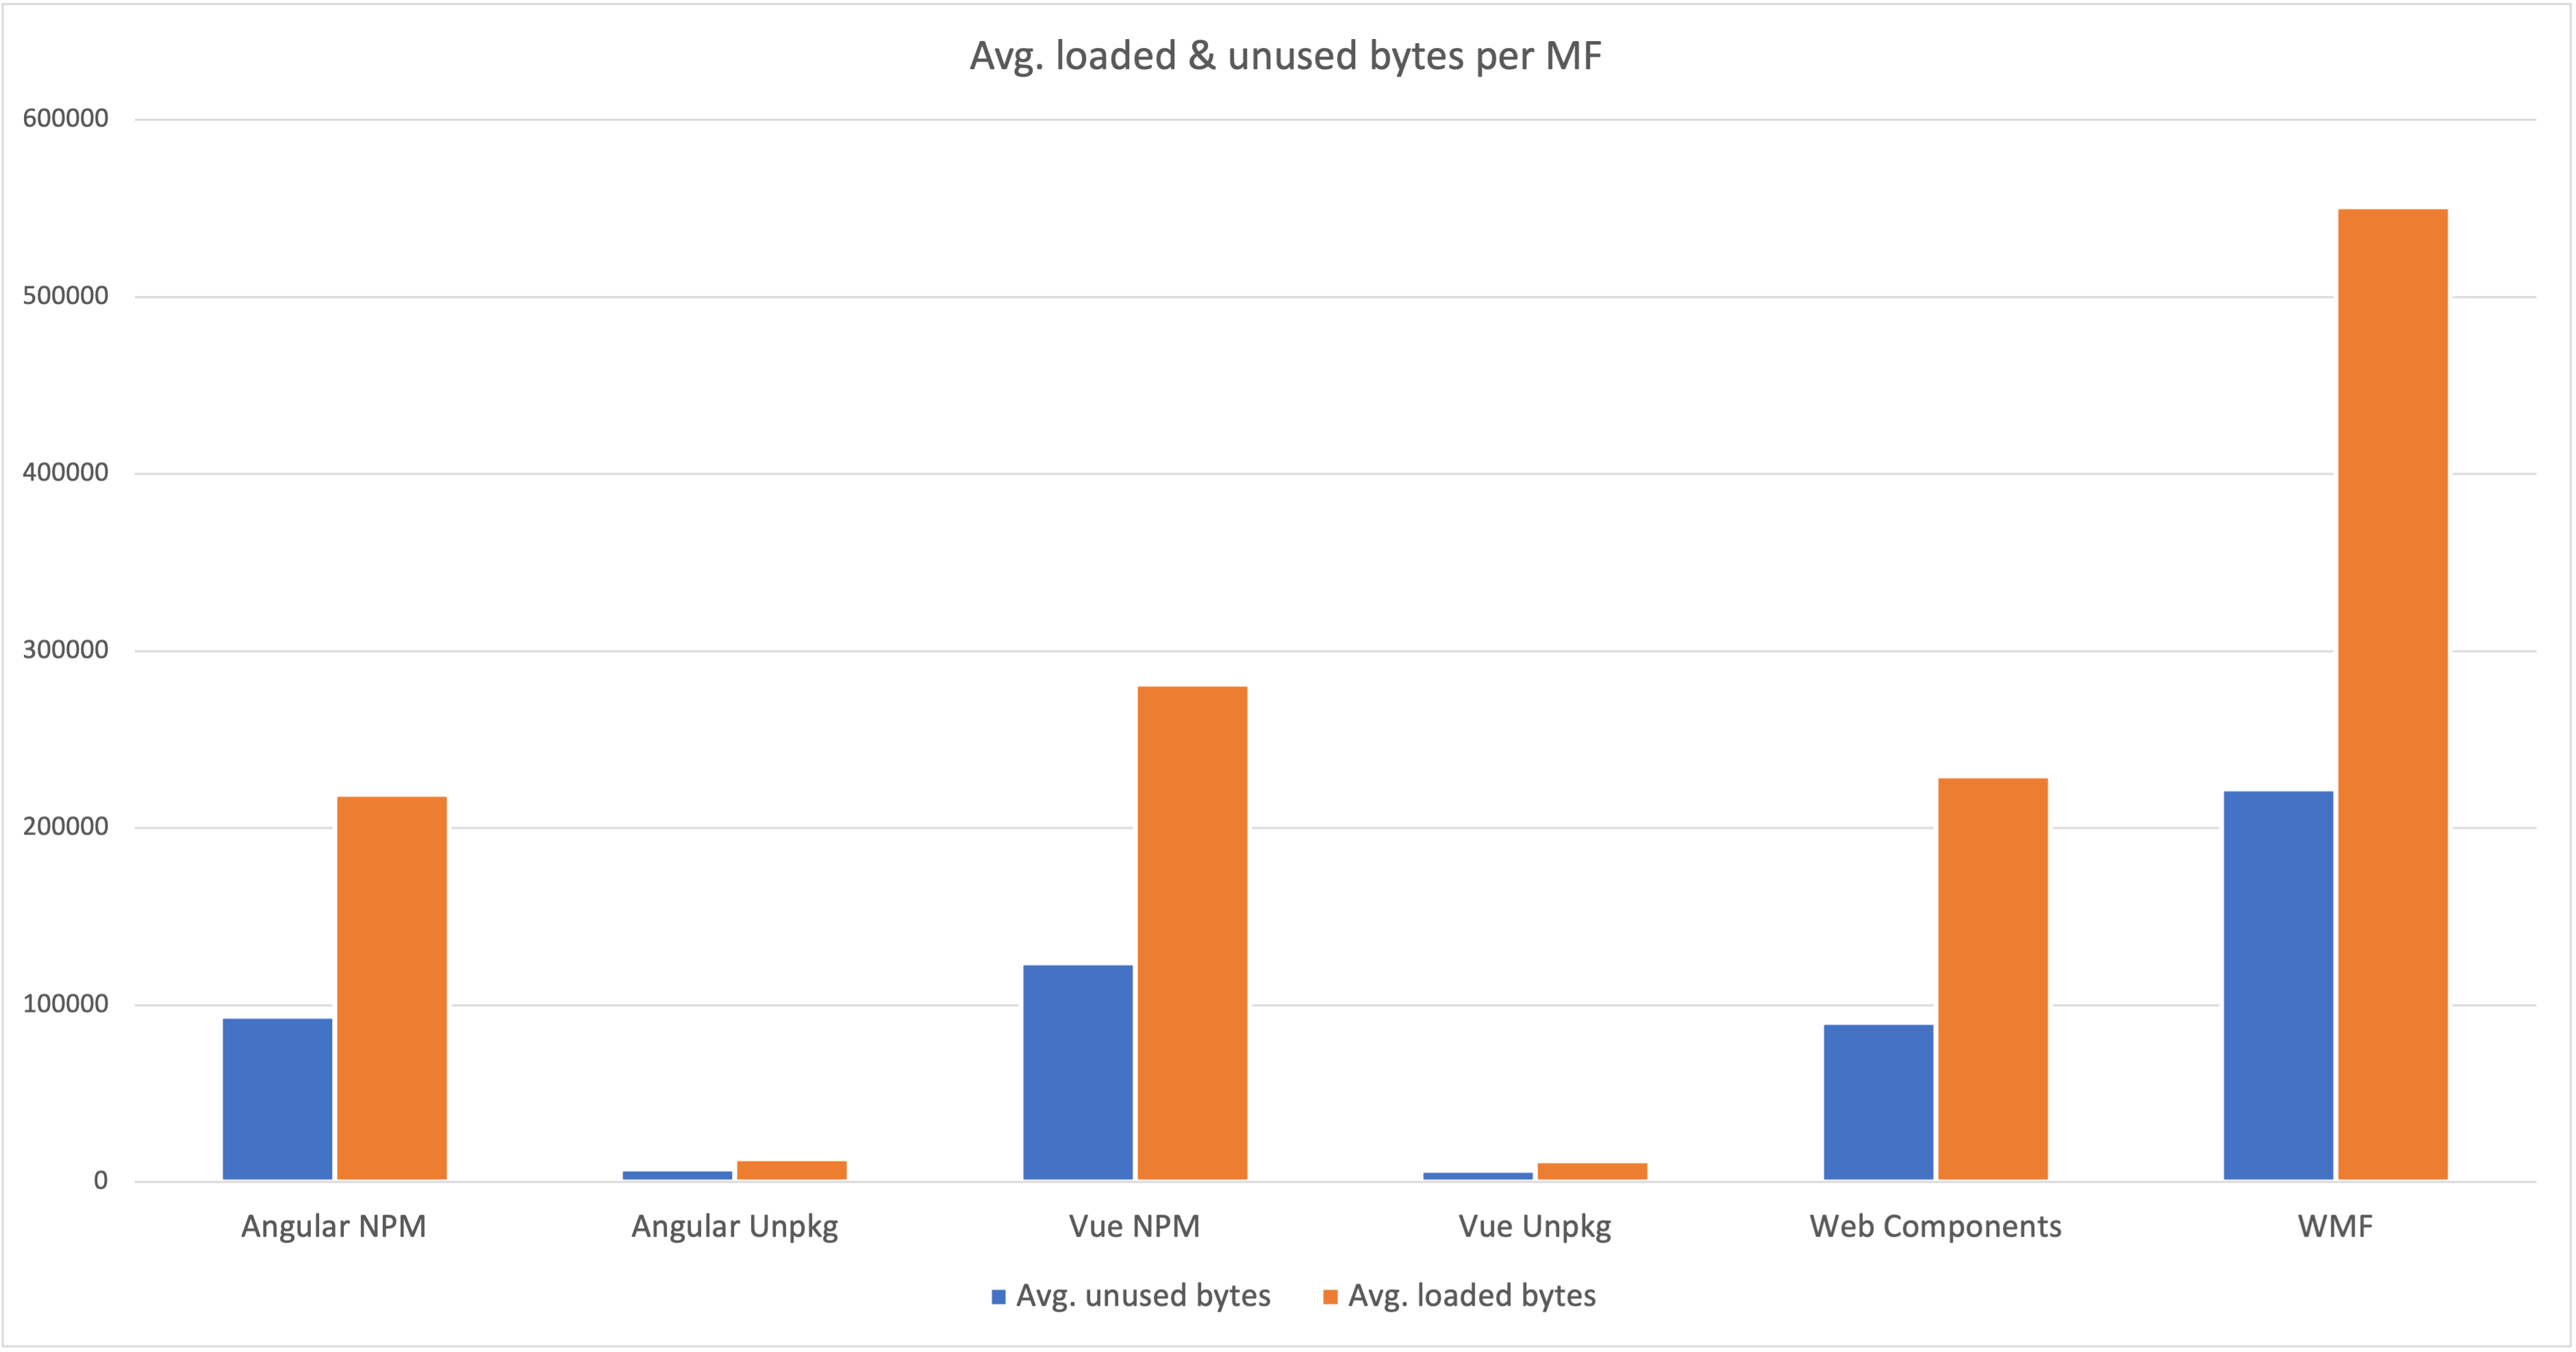
\includegraphics[width=1\textwidth]{Figures/avg_unsed_imported_1.png}
	\caption{Unused and imported bytes per landscape}
	\label{fig:unsed_imported_1}
\end{figure}

%\begin{figure}[!h]
%	\centering
%	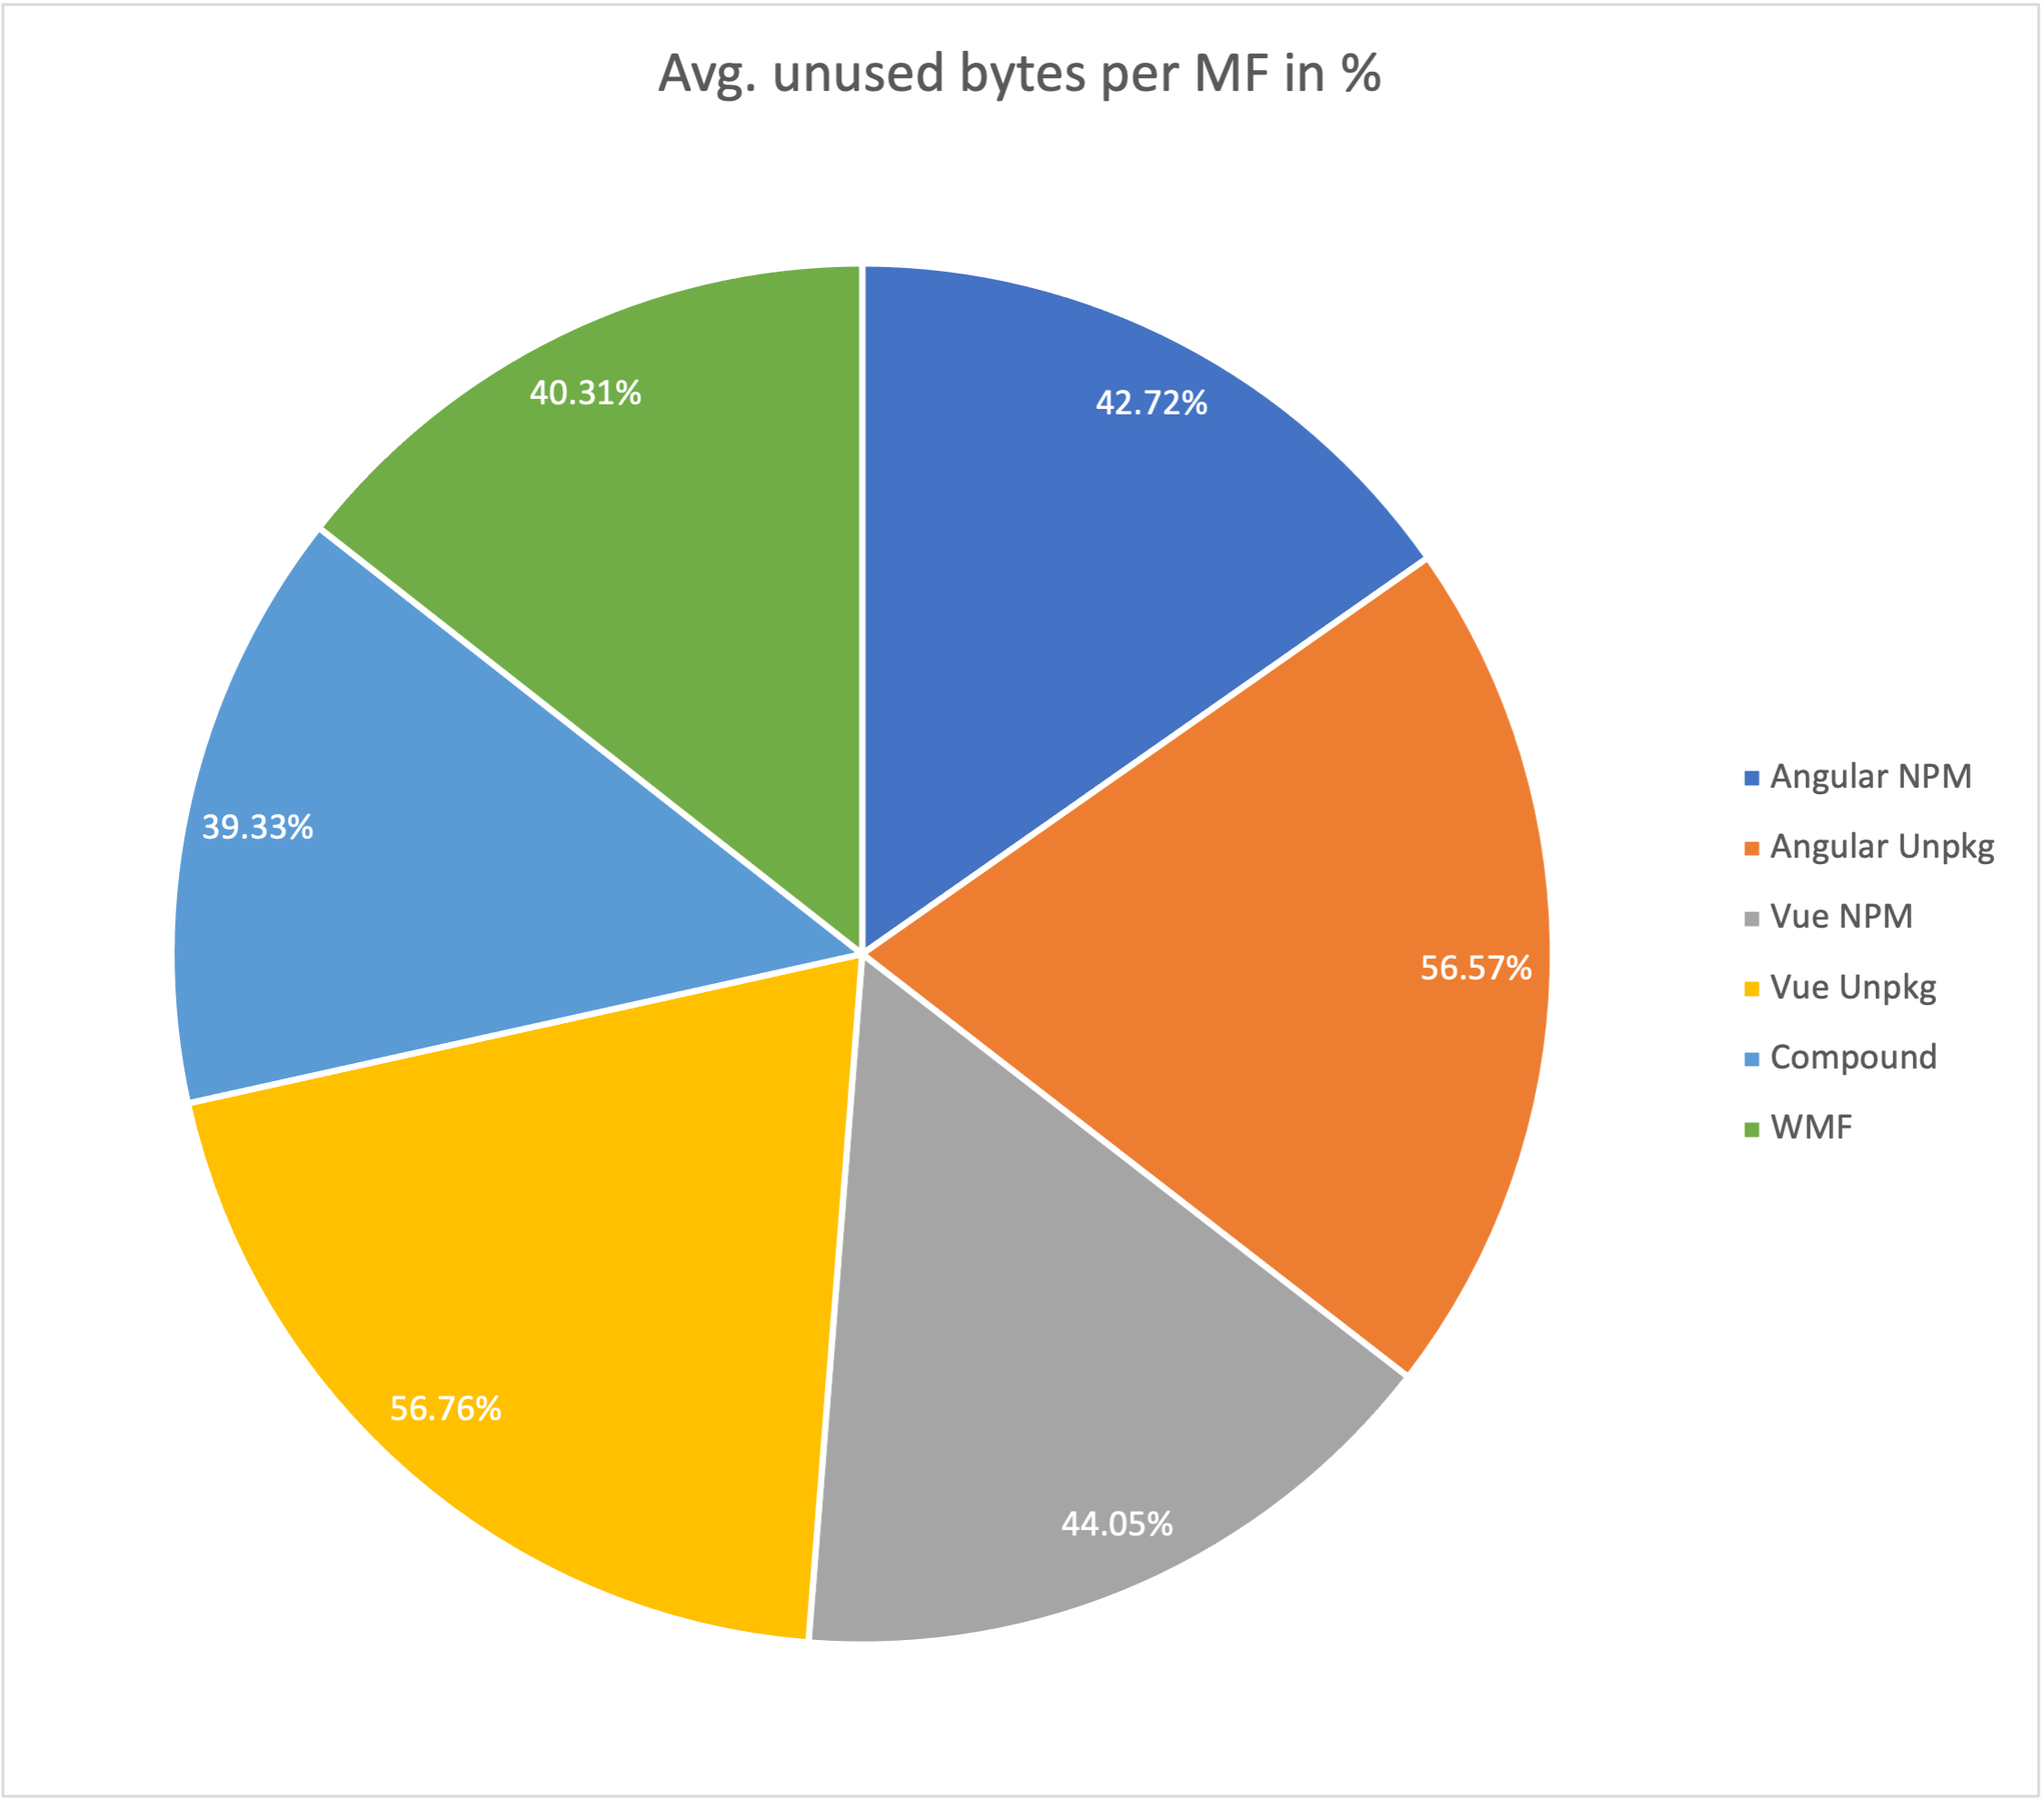
\includegraphics[width=1\textwidth]{Figures/avg_unsed_imported_2.png}
%	\caption{Unused and imported bytes per landscape in \%}
%	\label{fig:unsed_imported_2}
%\end{figure}

\normalsize
The data in table \ref{tab:lighthouse_used_report} and figure \ref{fig:unsed_imported_1} is highly application-dependent. 
As these landscapes are considered to be generally representative, a display in efficiency can be drawn from the charts.
The Unpkg CDN Nodes show a high ratio of unused bytes. 
However, it has to be taken into account that the overall imported sum of bytes is lower compared to the NPM counterparts, since only the required resources were requested from the CDN.
For the WMF Nodes, it can be argued that due to the bundling with Webpack, a lot of bytes were imported and only a few of them were not used. 
This can be explained by how the Module Federation was configured for this prototype. 
To simulate a multi-version landscape, a rather restrictive WMF configuration was required. 
Therefore, the majority of the bundled dependencies is actually used by the modules in those landscapes.
Web Components have the lowest unused bytes ratio of all the Nodes. 
This might be due to the fact that no UI framework was used for development. 
Therefore, no unnecessary framework features are present in this landscape.

The following chapter will draw conclusions based on the displayed data. Detailed tables, code examples and further information can be found in the archive.

	% \glsresetall
\chapter{Prospect} % Main chapter title
\label{Chapter8}

\lhead{Chapter 8. \emph{Prospect}}

The time available for the research, data collection and the actual writing was limited and therefore this transcript is scoped to a certain degree. Nonetheless the statements stated in this document are not final and further possibilities can be explored in that field. One of which was mentioned in the last chapter, the combinational effect of the researched technologies. A Web Components base micro frontend landscape, where the resources for the components are provided by a CDN for instance. Also the WMF topic was analyzed in the context of the UI framework Angular, this is a valid way of doing but the Module Federation can be used in combination with other frameworks as well. This is a field which also could be looked into, especially when taken into account that the data displayed in \ref{Chapter6} shows that a framework affects the performance of a micro frontend to a certain degree.
Another field which could not be explored in the time given for this document, is the development of an own CDN. Even though a approximate assumption was made concerning the effort connected to such a project, this is by no means empiric data. Therefore since the developed landscape rely on the Unpkg API to request the CDN  resources, it would an interesting experiment if and how an own CDN could improve or optimize the performance metrics for similar landscapes.
Lastly the Surge web server, used for the deployment of the landscapes, was connected to certain limitation too. Namely, the missing HTTP/2 server configuration. Thus, it would make sense to deploy those landscapes over different web servers just to see if the changes on server side improve the performances in the given context.

It is save to say, the landscape implemented can be considered to be representative but still offers room for improvement and optimization. Thus, when the given research is applied to a real life scenario, special conditions or requirements have to be considered when making a decision in that context. Therefore, it is mentioned in chapter \ref{Chapter7} that the gain or benefit of each respective technology is highly dependent on the individual use case.





	% \glsresetall
\chapter{Prospect} % Main chapter title
\label{Chapter9}

\lhead{Chapter 9. \emph{Prospect}}

The time available for the research, data collection and the actual writing was limited and therefore this transcript is scoped to a certain degree. Nonetheless the statements in this document are not final and further possibilities can be explored in that field. One of which was mentioned in the last chapter: The combinational effect of the researched technologies. For instance, a Web Component based micro frontend landscape, in which the resources for the components are provided by a CDN. Also the WMF topic was analyzed in the context of the UI framework Angular. Even though it is a valid way of doing, the Module Federation can be used in combination with other frameworks too. This is definitely a field which should be looked into. Especially when taking into account that it was shown, that a framework affects the performance of a micro frontend. 
Another field which was not dealt with, is the development of an own CDN. Even though a approximate assumption was made concerning the effort connected to such a project, this is by no means empiric data. Therefore since the developed landscape rely on the Unpkg.com API to request the CDN resources, it would be an interesting experiment if and how an own CDN could improve or optimize the performance metrics for similar landscapes.
Lastly the Surge web server, used for the deployment of the landscapes, was connected to certain limitations too, namely the missing HTTP/2 server configuration. Thus, it would make sense to deploy those landscapes over different web servers just to see if the changes on server-side improve the performances in the given context.

Event though, the prototypes are asserted to be representative, they still offer room for improvements and optimizations. Thus, when the given research is applied to a real life scenario, special conditions or requirements have to be considered when making a decision in that context. Therefore, it is mentioned in chapter \ref{Chapter7} that the gain or benefit of each respective technology is highly dependent on the individual use case. 

Nonetheless, the evidence provided in this transcript, is applicable for a development team, either as a source for advice, a documentation for best practices or as a basis for design decisions. The goal set for this thesis, can be considered to be achieved and exceeded, since it was showcased that the used technologies provide a solution for the issue of redundant libraries in micro frontend landscapes and how they do it. Additionally, it was also evaluated under which circumstances, those technologies are applicable under consideration of their own individual attributes. Based on this research, the mentioned aspects of the technologies can be explored and improved upon.





	
	
	\newpage
	%----------------------------------------------------------------------------------------
	%	BIBLIOGRAPHY
	%----------------------------------------------------------------------------------------
	
	\label{Sources}
	\lhead{}
	\begingroup
	\raggedright
	\addcontentsline{toc}{chapter}{Bibliography}
	\bibliographystyle{unsrt} % Use the "unsrtnat" BibTeX style for formatting the Bibliography
	\bibliography{sources} % The references (bibliography) information are stored in the file named "Bibliography.bib"
	\endgroup
	
	%----------------------------------------------------------------------------------------
	%	THESIS CONTENT - APPENDICES
	%----------------------------------------------------------------------------------------
	
	
	\listoffigures % Write out the List of Figures
	
	%\listoftables % Write out the List of Tables
	
	%----------------------------------------------------------------------------------------
	%	ABBREVIATIONS
	%----------------------------------------------------------------------------------------
	
	\clearpage % Start a new page
	
	\setstretch{1.5} % Set the line spacing to 1.5, this makes the following tables easier to read
	
	\lhead{\emph{Abbreviations}} % Set the left side page header to "Abbreviations"
	\listofsymbols{ll} % Include a list of Abbreviations (a table of two columns)
	{
		\textbf{API} & \textbf{A}pplication \textbf{P}rogramming \textbf{I}nterface \\
		\textbf{WMF} & \textbf{W}ebpack \textbf{M}odule \textbf{F}ederation \\
		\textbf{WC} & \textbf{W}eb \textbf{C}omponent \\
		\textbf{CDN} & \textbf{C}ontent \textbf{D}elivery \textbf{N}etwork \\
		\textbf{DOM} & \textbf{D}ocument \textbf{O}bject \textbf{M}odell \\
		\textbf{PoP} & \textbf{P}oint \textbf{o}f \textbf{P}resence \\
		\textbf{RTT} & \textbf{R}ound \textbf{T}rip \textbf{T}ime \\
	}
	
	\appendix % Cue to tell LaTeX that the following 'chapters' are Appendices
	
	% Include the appendices of the thesis as separate files from the Appendices folder
	% Uncomment the lines as you write the Appendices
	
	% Appendix Template

\chapter{Table of contents for the archive} % Main appendix title

\label{appendix1} % Change X to a consecutive letter; for referencing this appendix elsewhere, use \ref{AppendixX}

\lhead{Table of contents for the archive} 

\section{Folder Data}

Contains all data collected via the data collection process of chapter \ref{Chapter7}.

\subsection{analysisExcel.xlsm}

Central excel containing all calculation, graphs and data gathered via the testing process. 

\subsection{centralJson.csv}

Aggregated \texttt{.json} file, of all Lighthouse reports. 

\subsection{createAllCsv.sh}

Shell script, used to run a cascading process for the shell scripts in the sub-folders. 
Via this script, the generation of \textbf{analysisExcel.xlsm} and \textbf{centralJson.csv} is triggered.
 
\subsection{Folder angular-npm-data}

Folder containing all the data for the Angular NPM landscapes. 
The data is available as \texttt{.har}, \texttt{.json} as well as \textbf{.csv} files. 
The files themselves are split into, whether the data was collected with cache enabled or disabled.
Additionally, aggregated files for that landscapes are present, as well as a shell script to trigger the creations of every file in the folder.

\subsection{Folder angular-unpkg-data}

Folder containing all the data for the Angular Unpkg landscapes. 
The data is available as \texttt{.har}, \texttt{.json} as well as \textbf{.csv} files. 
The files themselves are split into, whether the data was collected with cache enabled or disabled.
Additionally, aggregated files for that landscapes are present, as well as a shell script to trigger the creations of every file in the folder.

\subsection{Folder vue-npm-data}

Folder containing all the data for the Vue NPM landscapes. 
The data is available as \texttt{.har}, \texttt{.json} as well as \textbf{.csv} files. 
The files themselves are split into, whether the data was collected with cache enabled or disabled.
Additionally, aggregated files for that landscapes are present, as well as a shell script to trigger the creations of every file in the folder.

\subsection{Folder vue-unpkg-data}

Folder containing all the data for the Vue Unpkg landscapes. 
The data is available as \texttt{.har}, \texttt{.json} as well as \textbf{.csv} files. 
The files themselves are split into, whether the data was collected with cache enabled or disabled.
Additionally, aggregated files for that landscapes are present, as well as a shell script to trigger the creations of every file in the folder.

\subsection{Folder compound-views-vanilla-data}

Folder containing all the data for the WC landscapes. 
The data is available as \texttt{.har}, \texttt{.json} as well as \textbf{.csv} files. 
The files themselves are split into, whether the data was collected with cache enabled or disabled.
Additionally, aggregated files for that landscapes are present, as well as a script to trigger the creations of every file in the folder.

\subsection{Folder wmf-views-data}

Folder containing all the data for the WMF landscapes. 
The data is available as \texttt{.har}, \texttt{.json} as well as \textbf{.csv} files. 
The files themselves are split into, whether the data was collected with cache enabled or disabled.
Additionally, aggregated files for that landscapes are present, as well as a shell script to trigger the creations of every file in the folder.

\section{Folder Master\_Development}

Containing all the developed prototype projects for this thesis. 

\subsection{Folder master\_thesis\_dev}

Contains the project for the CDN/NPM landscapes and their respective React Core application.

\subsection{Folder master\_thesis\_dev\_compound}

Contains the projects for the WC compounds landscapes.

\subsection{Folder master\_thesis\_dev\_wmf}

Contains the projects for the WMF compounds landscapes.

\subsection{Folder master\_thesis\_express\_app}

An express app, was developed in the early stages of the thesis and later abandoned, since a local data source was picked.

\section{Folder Self-developed-Scripts}

Contains all self-developed scripts for generating the \texttt{.csv} from the \texttt{.har} and \texttt{.json} files.

\subsection{Folder centralJson2Csv}

Generates the centralJson.csv file in the archive. It is a JavaScript script, which adds a command to the console, which is later executed via the shell scripts in the Data directory.

\subsection{Folder har2csv}

Generates a single \texttt{.csv} file based on single \texttt{.har} file. It is a JavaScript script, which adds a command to the console, which is later executed via the shell scripts in the Data directories.

\subsection{Folder hars2csvs}

Generates a single \texttt{.csv} file based on all \texttt{.har} files in the given directory. It is a JavaScript script, which adds a command to the console, which is later executed via the shell script in the Data directories to generate the central \texttt{.csv} files for each data directory.

\subsection{Folder json2Csv}

Generates a single \texttt{.csv} file based on single \texttt{.json} file. It is a JavaScript script, which adds a command to the console, which is later executed via the shell scripts in the Data directories.

\subsection{Folder jsons2Csvs}

Generates a single \texttt{.csv} file based on all \texttt{.json} files in the given directory. It is a JavaScript script, which adds a command to the console, which is later executed via the shell script in the Data directories to generate the central \texttt{.csv} files for each data directory.


	% Appendix Template

\chapter{Appendix 2} % Main appendix title

\label{appendix2} % Change X to a consecutive letter; for referencing this appendix elsewhere, use \ref{AppendixX}

\lhead{Lighthouse result tables} % Change X to a consecutive letter; this is for the header on each page - perhaps a shortened title

\section{Lighthouse result tables}

\begin{figure}[!h]
	\centering
	\begin{adjustbox}{width=\textwidth,totalheight=0.7\textheight}
		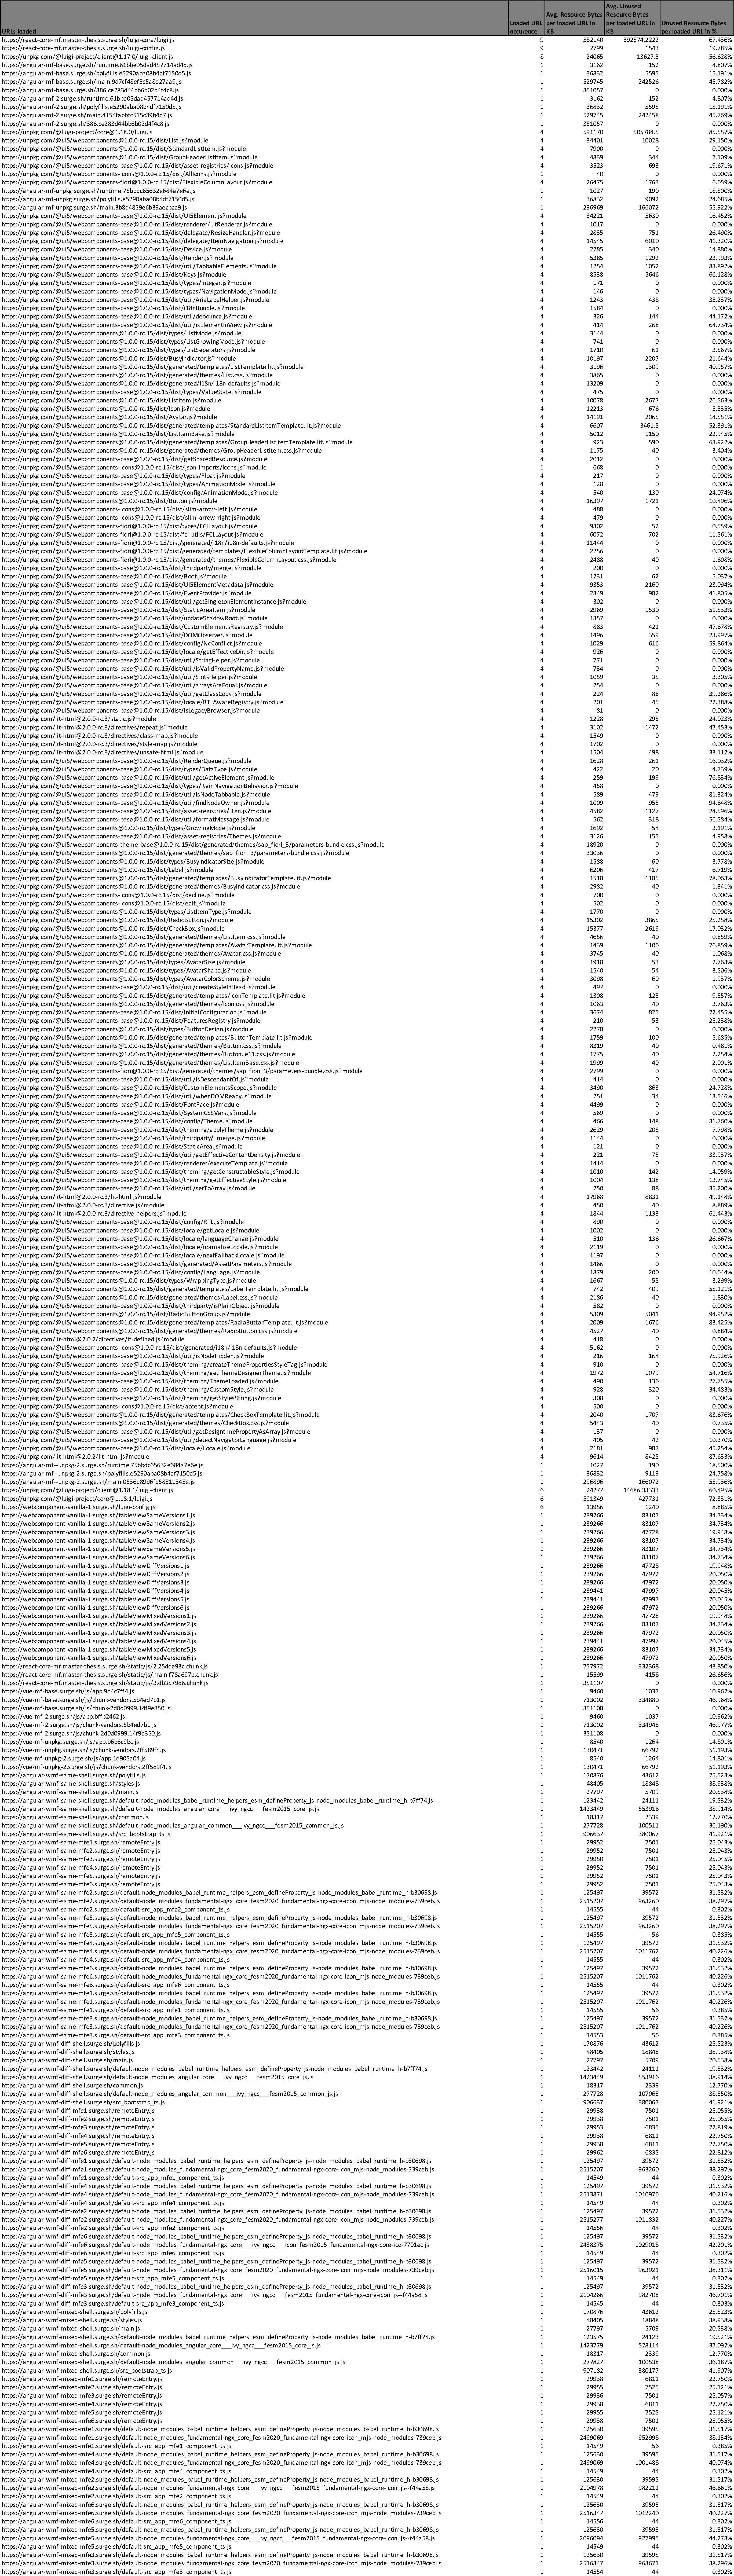
\includegraphics[angle=90]{Figures/lighthouse_json_1.pdf}
	\end{adjustbox}
	\caption{Table of numerical results taken from the Lighthouse reports, containing the imported and unused bytes per URL}
	\label{fig:appendix_2_1}
\end{figure}
\newpage
\begin{figure}[!h]
	\centering
	\begin{adjustbox}{width=\textwidth}
		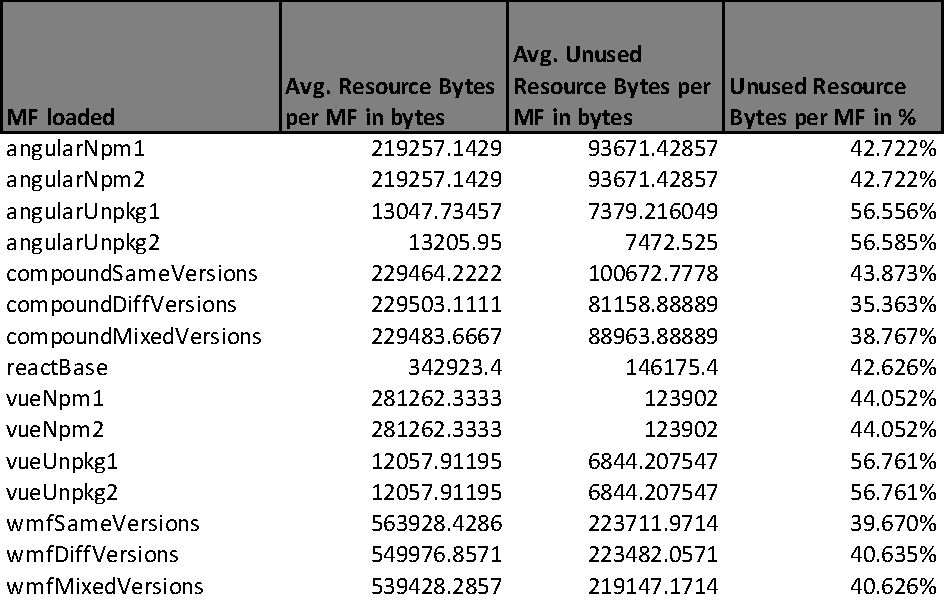
\includegraphics[]{Figures/lighthouse_json_2.pdf}
	\end{adjustbox}
	\caption{Table of numerical results taken from the Lighthouse reports, containing the imported and unused bytes per single MF}
	\label{fig:appendix_2_2}
\end{figure}



\begin{figure}[!h]
	\centering
	\begin{adjustbox}{width=\textwidth}
		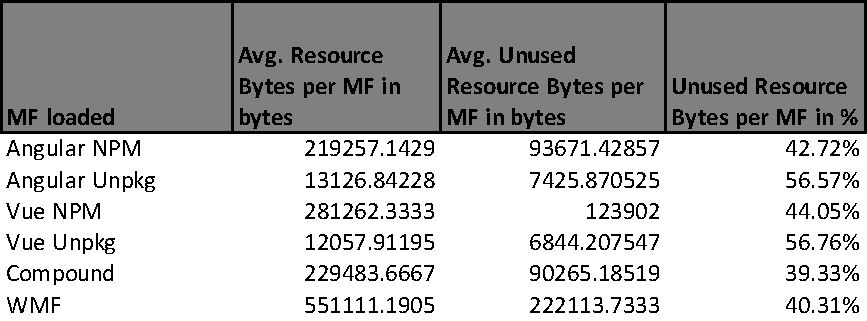
\includegraphics[]{Figures/lighthouse_json_3.pdf}
	\end{adjustbox}
	\caption{Table of numerical results taken from the Lighthouse reports, containing the imported and unused bytes per landscape}
	\label{fig:appendix_2_3}
\end{figure}
	% Appendix Template

\chapter{Appendix 3} % Main appendix title

\label{appendix3} % Change X to a consecutive letter; for referencing this appendix elsewhere, use \ref{AppendixX}

\lhead{Lighthouse result graphs} % Change X to a consecutive letter; this is for the header on each page - perhaps a shortened title

\section{Lighthouse result graphs}

\begin{figure}[!h]
	\centering
	\begin{adjustbox}{width=\textwidth,totalheight=0.7\textheight}
		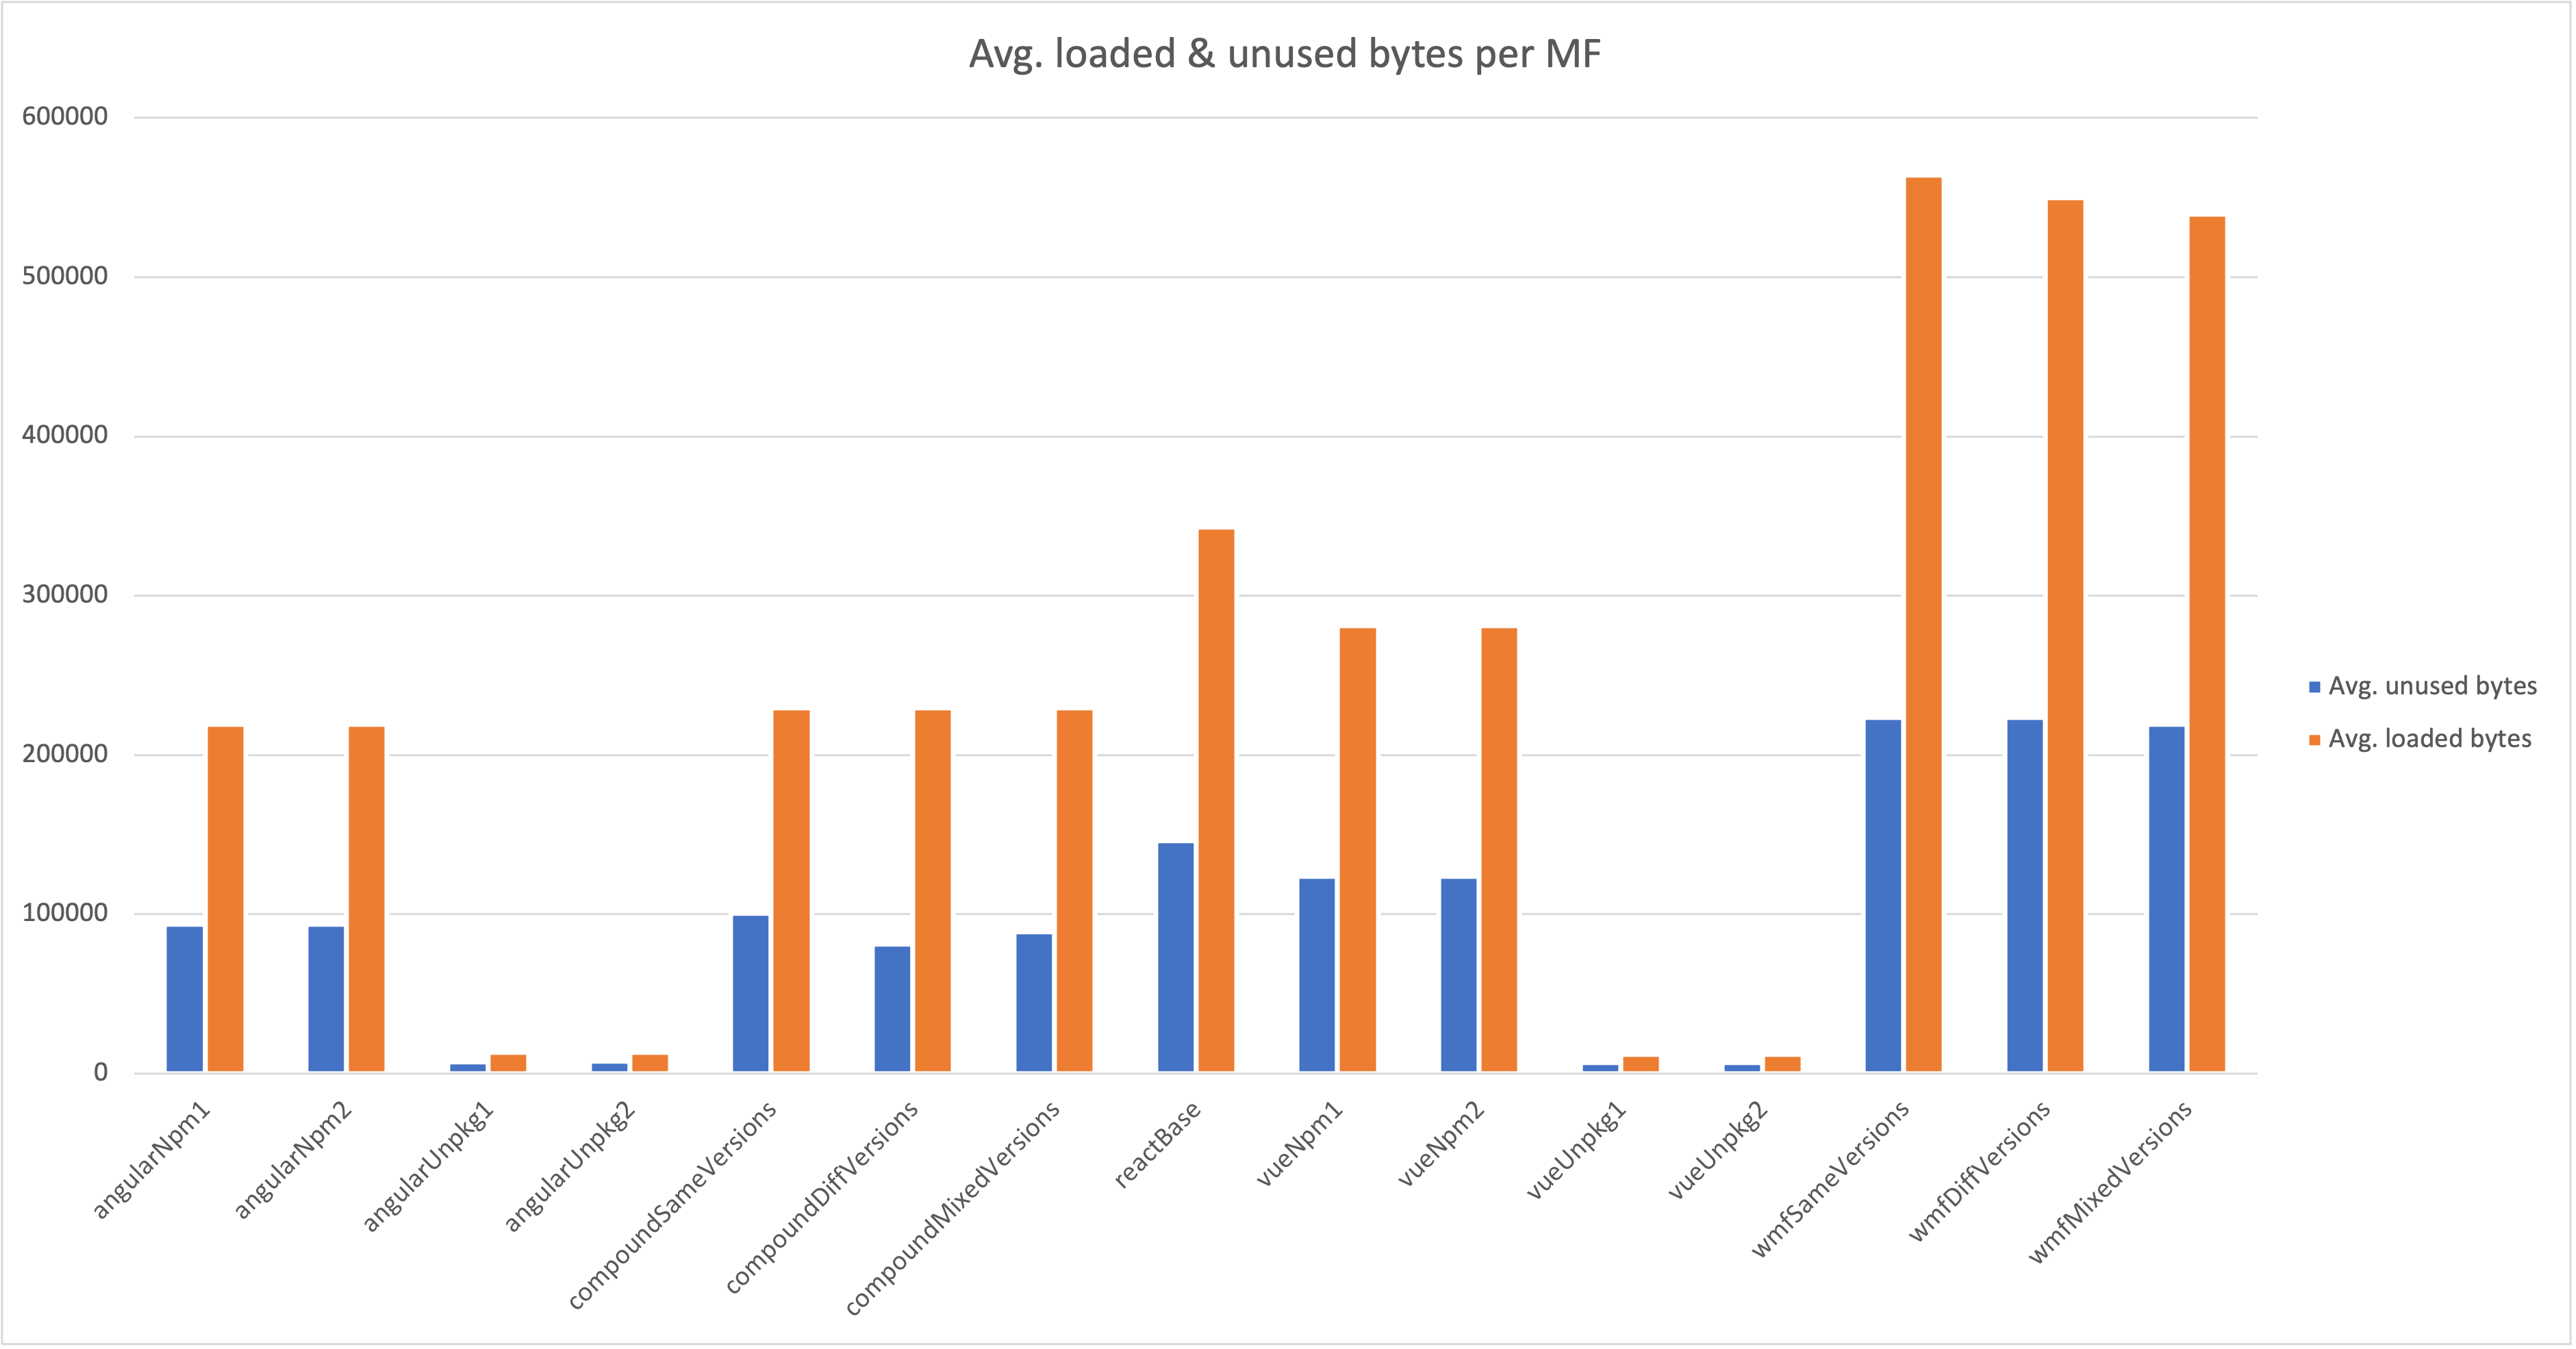
\includegraphics[angle=90]{Figures/avg_unsed_imported_mfe_1.png}
	\end{adjustbox}
	\caption{Bar chart for results taken from the Lighthouse reports, containing the imported and unused bytes per single MF}
	\label{fig:appendix_3_1}
\end{figure}
\newpage
\begin{figure}[!h]
	\centering
	\begin{adjustbox}{width=\textwidth,totalheight=\textheight}
		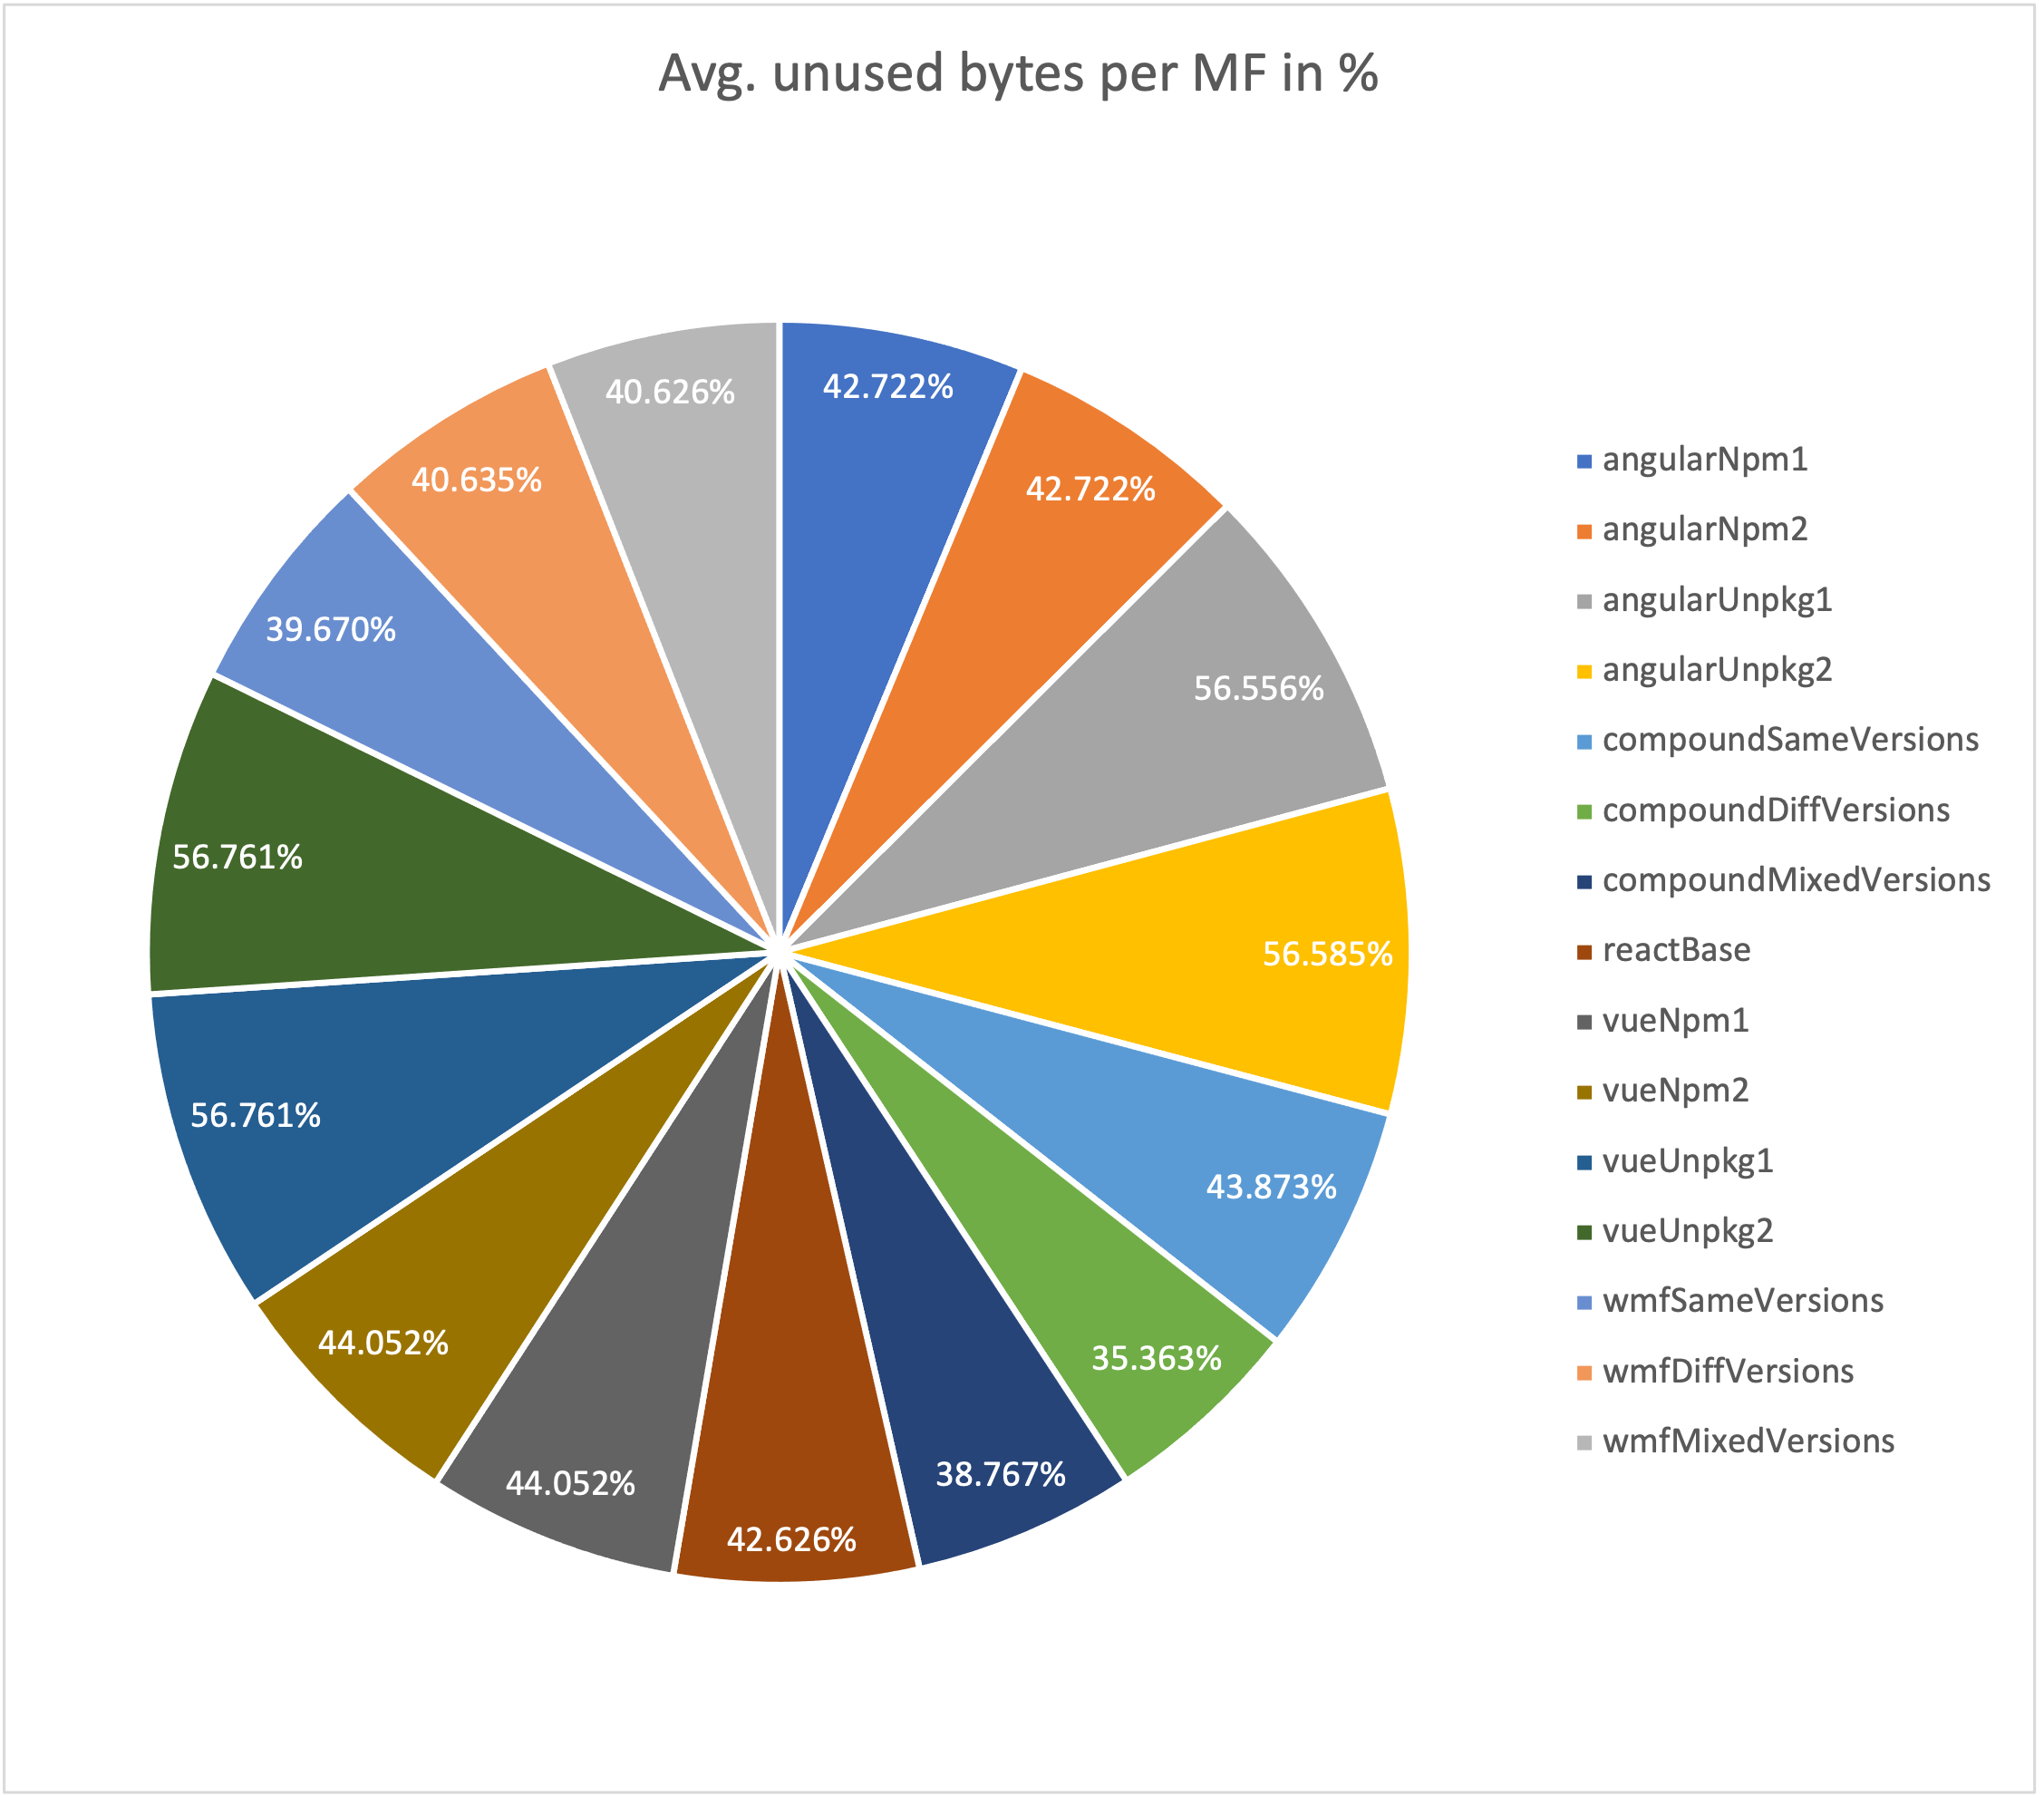
\includegraphics[angle=90]{Figures/avg_unsed_imported_mfe_2.png}
	\end{adjustbox}
	\caption{Pie chart for results taken from the Lighthouse reports, containing the unused bytes per single MF in \%}
	\label{fig:appendix_3_2}
\end{figure}
\newpage
\begin{figure}[!h]
	\centering
	\begin{adjustbox}{width=\textwidth,totalheight=\textheight}
		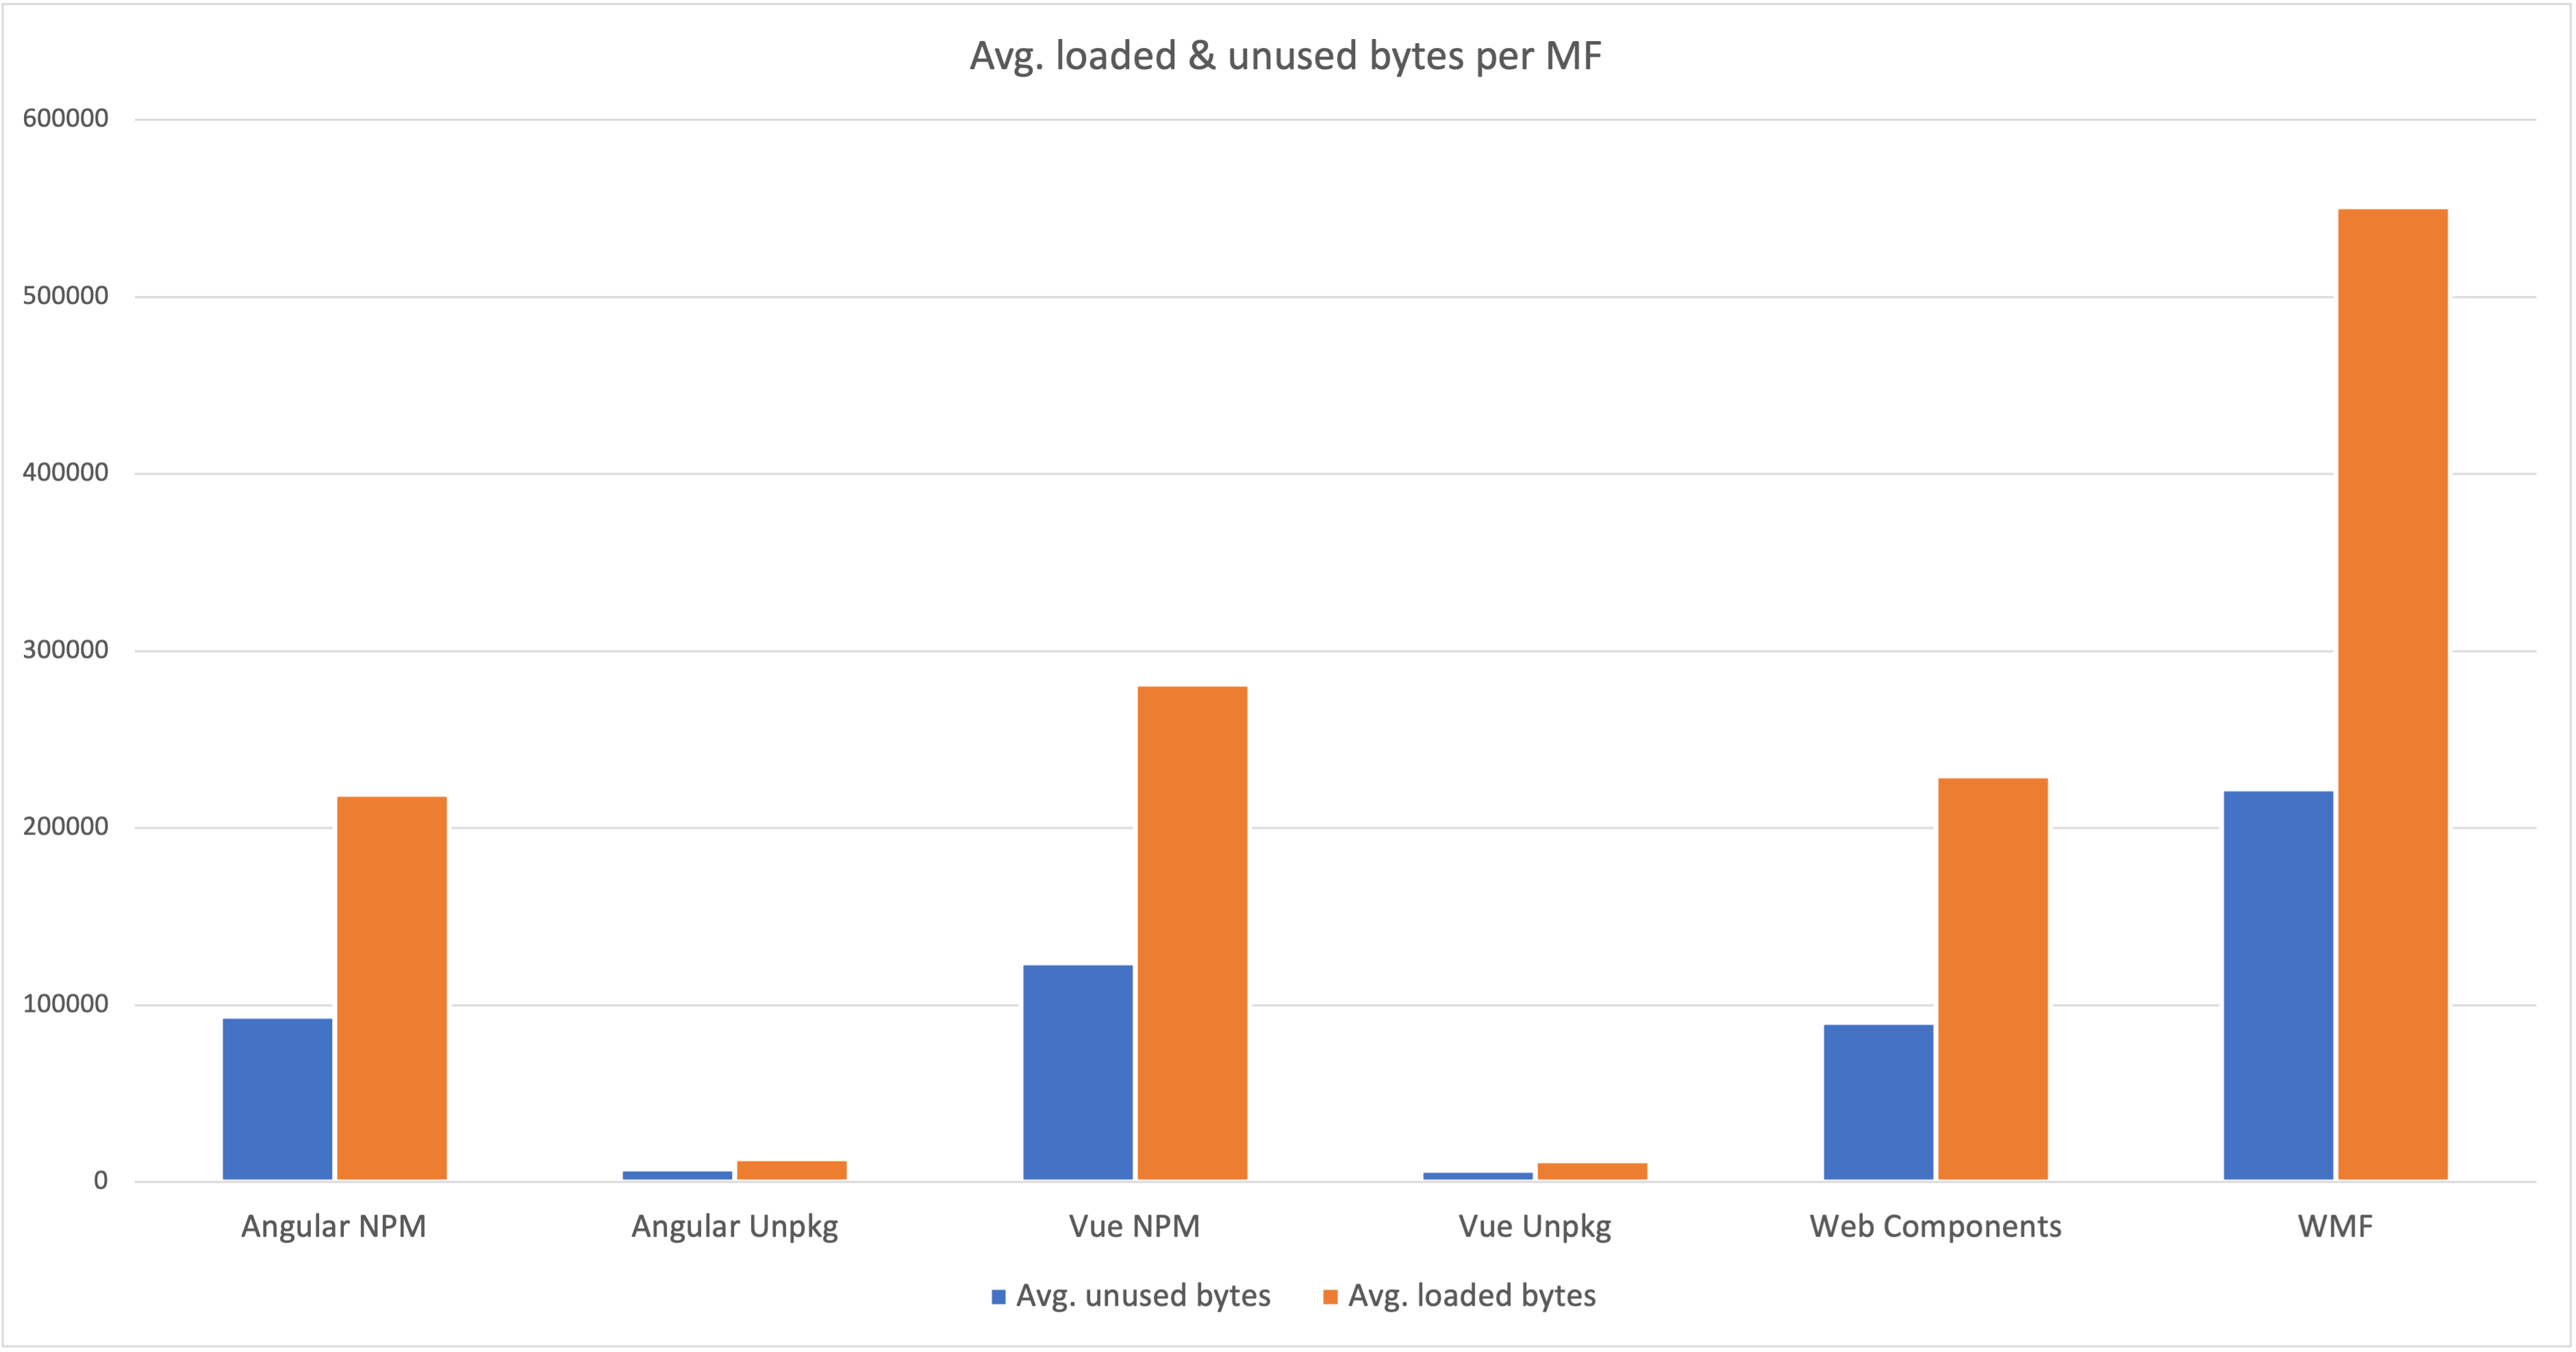
\includegraphics[angle=90]{Figures/avg_unsed_imported_1.png}
	\end{adjustbox}
	\caption{Bar chart for results taken from the Lighthouse reports, containing the imported and unused bytes per landscape}
	\label{fig:appendix_3_3}
\end{figure}
\newpage
\begin{figure}[!h]
	\centering
	\begin{adjustbox}{width=\textwidth,totalheight=\textheight}
		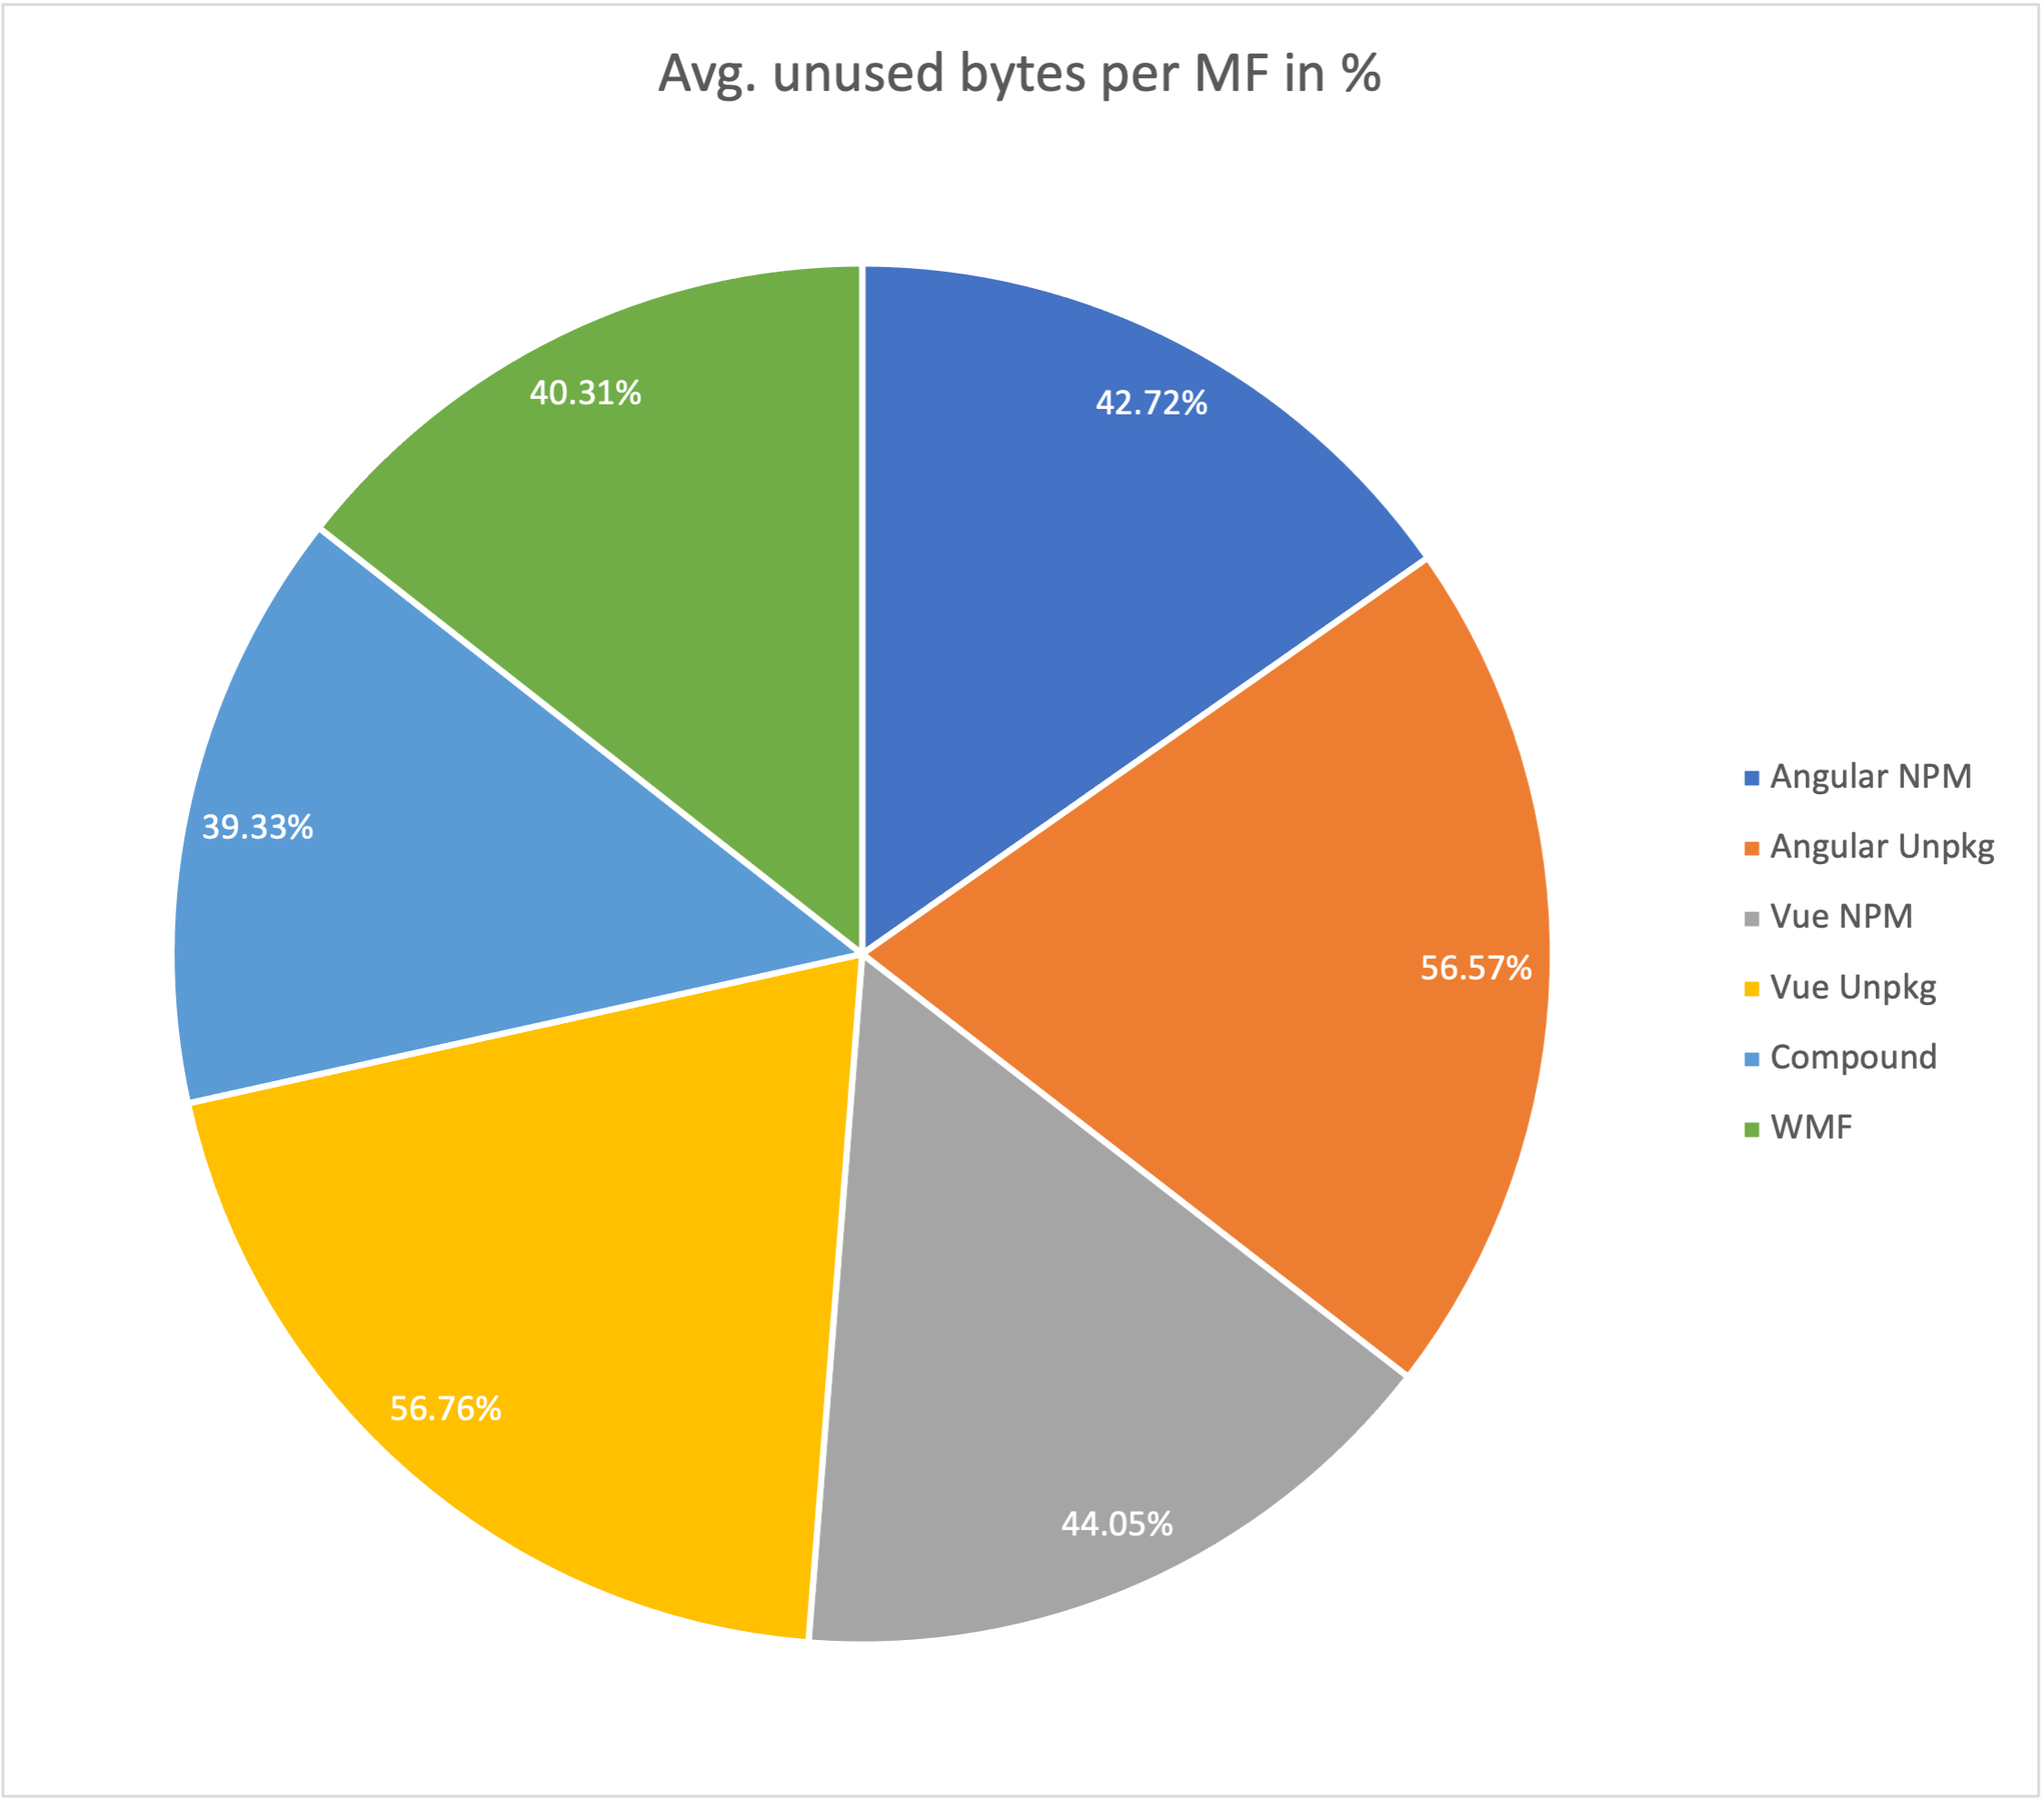
\includegraphics[angle=90]{Figures/avg_unsed_imported_2.png}
	\end{adjustbox}
	\caption{Pie chart for results taken from the Lighthouse reports, containing the unused bytes per landscape in \%}
	\label{fig:appendix_3_4}
\end{figure}
	
	\addtocontents{toc}{\vspace{2em}} % Add a gap in the Contents, for aesthetics
	
\end{document}
